\documentclass[11pt]{article}
\usepackage[numbers, compress, sort]{natbib}
\usepackage[margin=1.1in]{geometry}

\usepackage{float}
\usepackage[utf8]{inputenc} % allow utf-8 input
\usepackage[T1]{fontenc}    % use 8-bit T1 fonts
\usepackage{lmodern}
\usepackage{hyperref}       % hyperlinks  %[implicit=false, bookmarks=false]
\usepackage{url}            % simple URL typesetting
\usepackage{booktabs}       % professional-quality tables
\usepackage{amsfonts}       % blackboard math symbols
\usepackage{nicefrac}       % compact symbols for 1/2, etc.
\usepackage{microtype}      % microtypography
\usepackage[normalem]{ulem}
\usepackage{thm-restate}

\usepackage{mathtools, amsmath, amssymb, graphicx, verbatim, amsthm}
%\usepackage[thmmarks, thref, amsthm]{ntheorem}
\usepackage{color}
\definecolor{darkblue}{rgb}{0.0,0.0,0.2}
\definecolor{darkgreen}{rgb}{0.0,0.3,0.0}
\hypersetup{colorlinks,breaklinks,
            linkcolor=darkblue,urlcolor=darkblue,
            anchorcolor=darkblue,citecolor=darkblue}
\usepackage{wrapfig}
\usepackage[font=small]{caption}
\usepackage{subcaption}
\usepackage[colorinlistoftodos,textsize=tiny]{todonotes} % need xargs for below
%\usepackage{accents}
\usepackage{bbm}
\usepackage{xspace}

\usetikzlibrary{calc}
\newcommand{\Comments}{1}
\newcommand{\mynote}[2]{\ifnum\Comments=1\textcolor{#1}{#2}\fi}
\newcommand{\mytodo}[2]{\ifnum\Comments=1%
  \todo[linecolor=#1!80!black,backgroundcolor=#1,bordercolor=#1!80!black]{#2}\fi}
\newcommand{\raf}[1]{\mynote{darkgreen}{[RF: #1]}}
\newcommand{\raft}[1]{\mytodo{green!20!white}{RF: #1}}
\newcommand{\jessie}[1]{\mynote{teal}{[JF: #1]}}
\newcommand{\jessiet}[1]{\mytodo{teal!20!white}{JF: #1}}
\newcommand{\proposedadd}[1]{\mynote{orange}{#1}}
\newcommand{\bo}[1]{\mynote{blue}{[Bo: #1]}}
\newcommand{\botodo}[1]{\mytodo{blue!20!white}{[Bo: #1]}}
\newcommand{\btw}[1]{\mytodo{gray!20!white}{BTW: #1}}%TURN OFF FOR NOW \mytodo{gray}{#1}}
\ifnum\Comments=1               % fix margins for todonotes
  \setlength{\marginparwidth}{1in}
\fi


\newcommand{\reals}{\mathbb{R}}
\newcommand{\posreals}{\reals_{>0}}%{\reals_{++}}
\newcommand{\dom}{\mathrm{dom}}

\newcommand{\prop}[1]{\mathrm{prop}[#1]}
\newcommand{\eliccts}{\mathrm{elic}_\mathrm{cts}}
\newcommand{\eliccvx}{\mathrm{elic}_\mathrm{cvx}}
\newcommand{\elicpoly}{\mathrm{elic}_\mathrm{pcvx}}
\newcommand{\elicembed}{\mathrm{elic}_\mathrm{embed}}
\newcommand{\affhull}{\mathrm{affhull}}
\newcommand{\card}{\mathrm{card}}

\newcommand{\cell}{\mathrm{cell}}

\newcommand{\abstain}[1]{\mathrm{abstain}_{#1}}
\newcommand{\mode}{\mathrm{mode}}

\newcommand{\simplex}{\Delta_\Y}

% alphabetical order, by convention
\newcommand{\C}{\mathcal{C}}
\newcommand{\D}{\mathcal{D}}
\newcommand{\E}{\mathbb{E}}
\newcommand{\F}{\mathcal{F}}
\renewcommand{\H}{\mathcal{H}}
\newcommand{\I}{\mathcal{I}}
\renewcommand{\L}{\mathcal{L}}
\newcommand{\N}{\mathcal{N}}
\newcommand{\OP}{\mathcal{OP}}
\newcommand{\R}{\mathcal{R}}
\newcommand{\Sc}{\mathcal{S}}
\newcommand{\U}{\mathcal{U}}
\newcommand{\V}{\mathcal{V}}
\newcommand{\X}{\mathcal{X}}
\newcommand{\Y}{\mathcal{Y}}


\newcommand{\risk}[1]{\underline{#1}}
\newcommand{\inprod}[2]{\langle #1, #2 \rangle}%\mathrm{int}(#1)}
\newcommand{\inter}[1]{\mathring{#1}}%\mathrm{int}(#1)}
%\newcommand{\expectedv}[3]{\overline{#1}(#2,#3)}
\newcommand{\expectedv}[3]{\E_{Y\sim{#3}} {#1}(#2,Y)}
\newcommand{\toto}{\rightrightarrows}
\newcommand{\strip}{\mathrm{strip}}
\newcommand{\trim}{\mathrm{trim}}
\newcommand{\trimnonred}{\mathrm{trim}_{{\tt nonred}}}
\newcommand{\trimcover}{\mathrm{trim}_{\tt cover}}
\newcommand{\fplc}{finite-piecewise-linear and convex\xspace} %xspace for use in text
\newcommand{\conv}{\mathrm{conv}}
\newcommand{\indopp}{\bar{\mathbbm{1}}}
\newcommand{\ones}{\mathbbm{1}}
\DeclarePairedDelimiter\ceil{\lceil}{\rceil}

\newcommand{\Ind}[1]{\ones\{#1\}}

\newcommand{\hinge}{L_{\mathrm{hinge}}}
\newcommand{\ellzo}{\ell_{\text{0-1}}}
\newcommand{\ellabs}[1]{\ell_{#1}}
\newcommand{\elltopk}{\ell^{\text{top-$k$}}}
\newcommand{\elltop}[1]{\ell^{\text{top-$#1$}}}
\newcommand{\emb}{{\tt emb}}

\DeclareMathOperator*{\argmax}{arg\,max}
\DeclareMathOperator*{\argmin}{arg\,min}
\DeclareMathOperator*{\arginf}{arg\,inf}
\DeclareMathOperator*{\sgn}{sgn}

\newtheorem{theorem}{Theorem}
\newtheorem{lemma}{Lemma}
\newtheorem{proposition}{Proposition}
\newtheorem{corollary}{Corollary}
\newtheorem{conjecture}{Conjecture}

\newtheorem{definition}{Definition}
\newtheorem{remark}{Remark}
\newtheorem{assumption}{Assumption}


\title{An Embedding Framework for Consistent Polyhedral Surrogates}
%\title{Consistent Polyhedral Surrogates via Embeddings}
%\title{Convex Surrogates via Polyhedral Losses}
\author{%
 Jessie Finocchiaro \\
 \texttt{jefi8453@colorado.edu}\\
 CU Boulder
 \and
 Rafael Frongillo\\
 \texttt{raf@colorado.edu}\\
 CU Boulder
 \and
 Bo Waggoner\\
 \texttt{bwag@colorado.edu}\\
 CU Boulder
}

\begin{document}

\maketitle

\begin{abstract}
We formalize and study the natural approach of designing convex surrogate loss functions via embeddings for problems such as classification, ranking, or structured prediction. 
In this approach, one embeds each of the finitely many predictions (e.g. classes) as a point in $\reals^d$, assigns the original loss values to these points, and ``convexifies'' the loss in some way to obtain a surrogate.
We prove that this approach is equivalent, in a strong sense, to working with polyhedral (piecewise-linear convex) losses.
Moreover, given any polyhedral loss $L$, we give a construction of a link function through which $L$ is a consistent surrogate for the loss it embeds.
Our framework yields succinct proofs of consistency or inconsistency of various polyhedral surrogates in the literature, and for further reveals the target problems that inconsistent surrogates are consistent for.
We also show \raf{Newer stuff}
\end{abstract}

%\begin{keywords}%
%  property elicitation, proper scoring rules, surrogate loss functions, embeddings
%\end{keywords}

\section{Introduction}\label{sec:intro}

%\raf{MOVED FROM SEC 2; maybe incorporate?}
%Often, for computational or other reasons, one is interested in a property $\gamma$ such as the mode, but wishes to elicit it by minimizing some other ``surrogate'' loss $L$ over some other space such as $\reals^d$, then mapping the result back to $\R$ using a link function.
%We now formalize this procedure.
%
%\jessie{ TODO Items 01 Mar 2021
%	\begin{itemize}
%		\item \sout{Reorg sections: \S 3 (Embeddings, matching risks, etc.), \S 5 (Calibrated link), Examples, \S 4 (Polyhedral losses: I.E. implies consistency) OR Main results (w/o proof), Examples, \S 3, \S 5, \S 4}
%		\item \sout{Flesh out and expand on Ordered Partition Example}
%		\item add paragraph of discussion on the requirements of polyhedral losses
%		\item Check proof and statement of Theorem~\ref{thm:poly-ie-implies-consistent} - Jessie, 17 Mar 21: took a look to brush up; Theorem~\ref{thm:ie-iff-embeds-refinement} can use a look too.
%		\item Try to make section~\ref{sec:poly-loss-embed} self-contained, moving up results from appendix 
%		\begin{itemize}
%		\item \sout{for now, move everything up except PDs}
%		\item see if you can isolate what exactly we need from PDs and state it as a new lemma (which is just about Bayes risks) \raf{*}
%		\item rethink proofs of Prop 1 and 2, see if we resolve the redundancy  \raf{*}
%		\end{itemize}
%		\item Make Cor 1 a Theorem: "For L polyhedral, ell discrete, L ind elic prop[ell] <==> L consistent wrt ell"
%\end{itemize}
%TODO Items summer 2020
%	\begin{itemize}
%		\item Formalize reverse implication proof of Proposition 1 with projections into the affine hull and back
%		\item Mention how our focus on polyhedral risks and general links extends DKR Section 3.1 (probably after Prop 1)
%		\item Replace Proposition 2 with Lemma 7?
%		\item Theorem~\ref{thm:discrete-loss-poly-embeddable}: move from n-dimensional construction to n-1 dimensional construction (or add n-1 dim construction in appendix if it gets too hairy?)
%	\end{itemize}}


Convex surrogate losses are a central building block in machine learning for finite prediction problems such as classification and structured prediction tasks.
A growing body of work seeks to design and analyze convex surrogates for given loss functions, and more broadly, understand the best empirical risk minimization bounds that can found for a surrogate, for which consistency is a necessary condition.
For example, recent work has developed tools to bound the prediction dimension of the surrogate, meaning the dimension of the range of the surrogate hypothesis~\cite{frongillo2015elicitation,  ramaswamy2016convex}\jessiet{I took dimension of the hypothesis space to be, e.g., the degree of the polynomial $k$ for $\H = \{h : |\X| \times k \to \reals\}$.  Not sure if we should change to surrogates prediction/report space?}\raft{Excellent point.  Changed to prediction dimension, with a bit of explanation.}
Yet in some cases these bounds are far from tight, such as for \emph{abstain loss} (classification with an abstain option)~\citep{bartlett2008classification,yuan2010classification,ramaswamy2016convex,ramaswamy2018consistent,zhang2018reject}.
Furthermore, the kinds of strategies available for constructing surrogates, and their relative power, are not well understood.

We augment this literature by studying a particularly natural approach for finding convex surrogates, wherein one ``embeds'' a discrete loss.
Specifically, we say a convex surrogate $L$ embeds a discrete loss $\ell$ if there is an injective embedding from the discrete reports (predictions) to a vector space such that (i) the original loss values are recovered, and (ii) a report is $\ell$-optimal if and only if the embedded report is $L$-optimal.
If this embedding can be extended to a calibrated link function, which roughly maps approximately $L$-optimal reports to $\ell$-optimal reports, then consistency follows~\citep{agarwal2015consistent}.
Common examples of this general construction include hinge loss as a surrogate for 0-1 loss and the abstain surrogate mentioned above~\citep{ramaswamy2018consistent}.


\raf{The old intro had just one more paragraph here, now commented out}
% Using tools from property elicitation, we show a tight relationship between such embeddings and the class of polyhedral (piecewise-linear convex) loss functions.
% In particular, by focusing on Bayes risks, we show that every discrete loss is embedded by some polyhedral loss, and every polyhedral loss function embeds some discrete loss.
% Moreover, we show that any polyhedral loss gives rise to a calibrated link function to the loss it embeds,
% thus giving a very general framework to construct consistent convex surrogates for arbitrary losses.


We prove that such an embedding scheme is intimitely related to the class of polyhedral (piecewise-linear and convex) loss functions.
In particular, every discrete target loss is embedded by a polyhedral surrogate.
Moreover, such an embedding gives rise to calibrated link function.
Our proofs give explicit constructions for the surrogate (\S~\ref{sec:poly-loss-embed}) and link (\S~\ref{sec:calibration}) given a discrete target loss.

\jessiet{Want these as restatables so the numbering is consistent?}
\begin{theorem}\label{thm:embed-poly-informal}
  Every discrete loss $\ell$ is embedded by some polyhedral loss $L$, and every polyhedral loss $L$ embeds some discrete loss $\ell$.
\end{theorem}

\begin{theorem}\label{thm:link-informal}
  Given any polyhedral loss $L$, let $\ell$ be the discrete target loss it embeds. There exists a link function $\psi$ such that $(L,\psi)$ is calibrated with respect to $\ell$.
\end{theorem}

To better understand existing polyhedral surrogates, we provide tools to find the discrete losses they embed (Corollary~\ref{cor:representative-embeds-restriction}).
In short, if one can identify a finite \emph{representative set} $\Sc$ of reports for a surrogate $L$, meaning $\Sc$ always contains an $L$-optimal report for any label distribution, then $L$ embeds $L|_\Sc$, the loss given by $L$ restricting to $\Sc$.
We apply these tools to several polyhedral surrogates which have been proposed recently (\S~\ref{sec:applications}), showing in some cases that they are inconsistent for the desired target, but are consistent for a different target: the discrete loss they embed.

Underpinning our results are several observations which formalize the idea that polyhedral losses ``behave like'' discrete losses.
For example, discrete losses have polyhedral Bayes risks (as the minimum of finitely many linear functions), and so do polyhedral losses (Lemma~\ref{lem:poly-loss-poly-risk}).
As a consequence, polyhedral losses always have finite representative sets, and restricting the loss to any such set is an embedding.

We also provide several observations beyond what is needed to prove our main results, which we view as conceptual contributions (\S~\ref{sec:min-rep-sets},~\ref{sec:poly-ie-consistency}).
Using tools from property elicitation, we show an equivalence between minumum reprosentative sets and ``non-redundancy'', wherein no report is dominated by another.
We further show that, while the minimum representative set is not always unique, the loss values associated with it are unique, giving rise to a natural ``trim'' operation on losses.
Finally, using our main results, we show the following result: when restricting to the class of polyhedral surrogates, indirect elicitation is both necessary and sufficient for consistency (Theorem~\ref{thm:poly-ie-implies-consistent}).

Taken together, we view our contribution as both conceptual and practical.
We uncover the remarkable structure of polyhedral surrogates, deepening our understanding of the relationship between surrogate and target losses.
This structure leads to a powerful new framework to design and analyze surrogate losses, which we apply to several examples.
We hope our framework will inspire new research, and we conclude with several exciting directions for future work.

% \jessie{Take out this paragraph?}
%We go on to initiate a study of \emph{embedding dimension}: the minimal dimension for a given discrete loss to be so embedded.
%Our results give a complete characterization in the case of dimension 1; that is, real-valued surrogates.
%We find that a discrete loss can be embedded in the real line if and only if it is order-sensitive, meaning there is an ordering of the predictions such that the loss increases as one moves away from the correct prediction.
%We show further that order-sensitivity characterizes the existence of \emph{any} real-valued convex surrogate, implying that embeddings lose no generality.
%We conclude with preliminary results in higher dimensions and other future directions.

\paragraph{Related works.}
The literature on convex surrogates focuses mainly on smooth surrogate losses~\citep{crammer2001algorithmic,bartlett2006convexity,bartlett2008classification, duchi2018multiclass, williamson2016composite, reid2010composite,menon2019multilabel,zhang2020convex,bao2020calibrated}.
Nevertheless, nonsmooth losses, such as the polyhedral losses we consider, have been proposed and studied for a variety of classification-like problems~\citep{yang2018consistency,yu2018lovasz,lapin2015top}.
Moreover,~\citet{zhang2020bayes} describe the impact of the hypothesis class has on consistency, and when consistency relative to the hypothesis class differs from Bayes consistency; the latter is what we describe in this paper when we say ``consistency.''

A notable addition to this literature is~\citet{ramaswamy2018consistent}, who argue that nonsmooth losses may enable dimension reduction of the prediction space (range of the surrogate hypothesis) relative to smooth losses, illustrating this conjecture with a surrogate for \emph{abstain loss} needing only $\log(n)$ dimensions for $n$ labels, whereas the best known smooth loss needs $n-1$ dimensions.
Their surrogate is a natural example of an embedding (cf.~\S~\ref{sec:abstain}), and serves as inspiration for our work.


While property elicitation has by now an extensive literature~\citep{savage1971elicitation,osband1985information-eliciting,lambert2008eliciting,gneiting2011making,steinwart2014elicitation,frongillo2015vector-valued,fissler2016higher,lambert2018elicitation}, these works are mostly concerned with point estimation problems.
Literature directly connecting property elicitation to consistency is sparse.
However,~\citet{agarwal2015consistent} consider single-valued properties in finite outcome settings, whereas finite properties elicited by general convex losses are necessarily set-valued.
\citet{finocchiaro2021unifying} additionally relates indirect property elicitation to consistency when one is given either a target loss or property in both discrete and continuous prediction settings, assuming surrogates attain their infimum in expectation over all distributions over the outcomes.

% \citet{agarwal2015consistent} and~\citet{ramaswamy2016convex} study the existence of convex surrogates; the latter proves lower bounds on dimensionality of hypothesis spaces for e.g.~0-1 loss via their notion of feasible subspace dimension.
%   These works are generally not directly comparable to our results, as they do not consider the embedding method.
%   However, we will mention relevant results inline.


\section{Setting}
\label{sec:setting}

For discrete prediction problems like classification, due to hardness of directly optimizing a given discrete loss, many machine learning algorithms minimize a surrogate loss function with better optimization qualities, e.g., convexity.
Of course, to show that this surrogate loss successfully addresses the original problem, one needs to establish consistency, which depends crucially on the choice of link function that maps surrogate reports (predictions) to original reports.
After introducing notation, and terminology from property elicitation, we study \emph{calibration} (Definition~\ref{def:calibrated}), which is equivalent to consistency in finite outcome settings~\citep{bartlett2006convexity,tewari2007consistency,ramaswamy2016convex} and depends solely on the conditional distribution over $\Y$.
Consistency is a prerequisite to obtain empirical risk minimization bounds, motivating our firm requirement of constructing consistent surrogates.

\subsection{Notation and Losses}
\label{sec:notation-losses}

Let $\Y$ be a finite label space, and throughout let $n=|\Y|$.
The set of probability distributions on $\Y$ is denoted $\simplex\subseteq\reals^{\Y}_+$, represented as vectors of probabilities (requiring $\|p\|_1 = 1$).
We write $p_y$ for the probability of outcome $y \in \Y$ drawn from $p \in \simplex$.
We first discuss the conditional setting, with just labels $\Y$ and no features $\X$, and show in \S~\ref{sec:calibration} how these notions relate to the usual $\X\times\Y$ setting considering features.

We assume that a given discrete prediction problem, such as classification, is given in the form of a \emph{discrete loss}\jessiet{discrete vs target?} $\ell:\R\to\reals^\Y_+$, which maps a report (prediction) $r$ from a finite set $\R$ to the vector of loss values $\ell(r) = (\ell(r)_y)_{y\in\Y}$ for each possible outcome $y\in\Y$.
We will assume throughout that the given discrete loss is \emph{non-redundant}, meaning every report is uniquely optimal (minimizes expected loss) for some distribution $p\in\simplex$.
Similarly, surrogate losses will be written $L:\reals^d\to\reals^\Y_+$, typically with reports written $u\in\reals^d$.
\btw{Cut generic loss}%(A generic loss will be written $L:\R\to\reals^\Y$.)
We write the corresponding expected loss when $Y \sim p$ as $\inprod{p}{\ell(r)}$ and $\inprod{p}{L(u)}$.
The \emph{Bayes risk} of a loss $L:\reals^d\to\reals^\Y_+$ is the function $\risk{L}:\simplex\to\reals_+$ given by $\risk{L}(p) := \inf_{u\in\reals^d} \inprod{p}{L(u)}$; naturally for discrete losses we write $\risk{\ell}$ with the infimum over $\R$.

%\jessie{In general, we shall denote discrete reports by $r \in \R$, and real-valued reports by $u \in \U$.}
For example, 0-1 loss is a discrete loss with $\R = \Y = \{-1,1\}$
given by $\ellzo(r)_y = \Ind{r \neq y}$, with Bayes risk $\risk{\ellzo}(p) = 1-\max_{y\in\Y} p_y$.
Two important surrogates for $\ellzo$ are hinge loss $\hinge(u)_y = (1-yu)_+$, where $(x)_+ = \max(x,0)$, and logistic loss $L(u)_y = \log(1+\exp(-yu))$ for $u\in\reals$.
See Figure~\ref{fig:bayes-risks-01} for a visualization of the Bayes risks of 0-1, Hinge, and Logistic losses, respectively.

Most of the surrogates $L$ we consider will be \emph{polyhedral}, meaning piecewise linear and convex; we therefore briefly recall the relevant definitions.
In $\reals^d$, a \emph{polyhedral set} or \emph{polyhedron} is the intersection of a finite number of closed halfspaces.
A \emph{polytope} is a bounded polyhedral set.
A convex function $f:\reals^d\to\reals$ is \emph{polyhedral} if its epigraph is polyhedral, or equivalently, if it can be written as a pointwise maximum of a finite set of affine functions~\citep{rockafellar1997convex}.
%
\begin{definition}[Polyhedral loss]
  A loss $L: \reals^d \to \reals^{\Y}_+$ is \emph{polyhedral} if $L(u)_y$ is a polyhedral (convex) function of $u$ for each $y\in\Y$.
\end{definition}
%
For example, hinge loss is polyhedral, whereas logistic loss is not.
To motivate our focus on polyhedral losses, we echo~\citet[Section~1.2]{ramaswamy2018consistent}, who note that smooth surrogates often encode much more information than necessary, and in these cases non-smooth surrogates are the best candidates to achieve a low input dimension $d$.

\subsection{Property Elicitation}
\label{sec:property-elicitation}

To make headway, we will appeal to concepts and results from the property elicitation literature, which elevates the \emph{property}, or map from distributions to optimal reports, as a central object to study in its own right.
In our case, this map will often be multivalued, meaning a single distribution could yield multiple optimal reports.
(For example, when $p=(1/2,1/2)$, both $r=1$ and $r=-1$ optimize 0-1 loss.)
To this end, we will use double arrow notation to mean a mapping to all nonempty subsets, so that $\Gamma: \simplex \toto \R$ is shorthand for $\Gamma: \simplex \to 2^{\R} \setminus \{\emptyset\}$.
%See the discussion following Definition~\ref{def:elicits} for notational conventions.% regarding $\R$, $\Gamma$, $\gamma$, $L$, $\ell$, etc.

\begin{definition}[Property, level set]\label{def:property}
  A \emph{property} is a function $\Gamma:\simplex\toto\R$.
  The \emph{level set} of $\Gamma$ for report $r$ is the set $\Gamma_r := \{p \in \simplex : r \in \Gamma(p)\}$.
\end{definition}

Intuitively, $\Gamma(p)$ is the set of reports which should be optimal for a given distribution $p$, and $\Gamma_r$ is the set of distributions for which the report $r$ should be optimal.
In general, by optimal, we mean minimizing an associated loss function in expectation over $p$, which we formalize shortly.
Note that our definitions align such that discrete losses elicit finite properties; both are non-redundant in the correct senses.
For example, the \emph{mode} is the %finite
property $\mode(p) = \argmax_{y\in\Y} p_y$, and captures the set of optimal reports for 0-1 loss: for each distribution over the labels, one should report the most likely label.
In this case we say 0-1 loss \emph{elicits} the mode, as we formalize below.
% This terminology comes from the information elicitation \jessiet{information vs property... do we care?}\raft{we could also say economics literature; not ``property'' though since that doesn't offer an explanation of the word ``elicits''} literature~\citep{savage1971elicitation,osband1985information-eliciting,lambert2008eliciting}, in which a report $r$ is elicited from some forecaster by scoring her with a loss on the observed outcome $y$.

\begin{definition}[Elicits]
  \label{def:elicits}
  A loss $L:\R\to\reals^\Y_+$, \emph{elicits} a property $\Gamma:\simplex \toto \R$ if
  \begin{equation}
    \forall p\in\simplex,\;\;\;\Gamma(p) = \argmin_{r \in \R} \inprod{p}{L(r)}~.
  \end{equation}
  As $L$ elicits a unique property, we write $\prop{L}$ to refer to the property elicited by a loss $L$.
\end{definition}

For finite properties (those with $|\R|<\infty$) and discrete losses, we will use lowercase notation $\gamma$ and $\ell$, respectively, with reports $r\in\R$; for surrogate properties and losses we use $\Gamma$ and $L$, with reports $u\in\reals^d$.
% For finite properties (those with $|\R|<\infty$) and discrete losses, we will use lowercase notation $\gamma:\simplex\toto\R$ and $\ell:\R\toto\reals^\Y_+$, respectively, with reports $r\in\R$; for surrogate properties and losses we use $\Gamma:\simplex\toto\reals^d$ and $L:\reals^d\toto\reals^\Y_+$, with reports $u\in\reals^d$.
For general properties and losses, we will also use $\Gamma$ and $L$, as above.

% Often we will work with two properties simultaneously, a finite property $\gamma:\simplex\toto\R$, and its embedded version $\Gamma:\simplex\toto\reals^d$.
% In this case, we write the embedded reports as $u\in\reals^d$, reserving $r\in\R$ for the finite property.

\subsection{Calibration and Links}
\label{sec:calibration}


To assess whether a surrogate and link function align with the original loss, we turn to the common condition of \emph{calibration}.
Roughly, a surrogate and link are calibrated if the best possible expected loss achieved by linking to an incorrect report is strictly suboptimal, which require that the excess loss of some report is bounded by (a constant times) the excess loss of the linked report.

% \begin{definition}[Consistency]\label{def:consistency}
%   A surrogate $L:\reals^d\to\reals^\Y_+$ and link $\psi:\reals^d\to\R$ is \emph{consistent} with a discrete loss $\ell:\R\to\reals^\Y_+$ if \raf{statement about distributions on $\X\times\Y$, limits of hypotheses, and Bayes opt hypotheses}
% \end{definition}

% \begin{definition}[Separated Link]\label{def:links}
%   Let discrete loss $\ell:\R\to\reals^\Y_+$ and surrogate $L:\reals^d\to\reals^\Y_+$ be given.
%   A \emph{link function} is a map $\psi:\reals^d\to\R$.
%   We say that a link $\psi$ is \emph{$\delta$-separated} for some $\delta > 0$ if for all $p \in \simplex$ and $u\in\reals^d$, we have
%   \begin{align*}
%     \inprod{p}{L(u)} - \inf_{u' \in \reals^d} \inprod{p}{L(u')} \geq \delta\left(\inprod{p}{\ell(\psi(u))} - \min_{r \in \R} \inprod{p}{\ell(r)}\right)~.
%   \end{align*}
%   A link is \emph{separated} if it is $\delta$-separated for some $\delta>0$.
% \end{definition}

\begin{definition}
  \label{def:calibrated}
  Let original loss $\ell:\R\to\reals^\Y_+$, proposed surrogate $L:\reals^d\to\reals^\Y_+$, and link function $\psi:\reals^d\to\R$ be given.
  We say $(L,\psi)$ is \emph{calibrated} with respect to $\ell$ if
for all $p \in \simplex$,
  \begin{equation}
    \label{eq:calibrated}
  \inf_{u \in \reals^d : \psi(u) \not\in \gamma(p)} \inprod{p}{L(u)} > \inf_{u \in \reals^d} \inprod{p}{L(u)}~.
  \end{equation}
  If $(L, \psi)$ is calibrated with respect to $\ell$, we call $\psi$ a \emph{calibrated link.}
\end{definition}
It is well-known in finite-outcome settings that calibration is equivalent to \emph{consistency}, in the following sense (cf.~\citep{agarwal2015consistent}).
Given feature space $\X$, fix a distribution $D \in \Delta(\X\times\Y)$.
Let $L^*$ be the best possible expected $L$-loss achieved by any hypothesis $H:\X\to\reals^d$, and $\ell^*$ the best expected $\ell$-loss for any hypothesis $h:\X\to\R$, respectively.
Then $(L,\psi)$ is consistent if a sequence of surrogate hypotheses $H_1,H_2,\ldots$ whose $L$-loss limits to $L^*$, then the $\ell$-loss of $\psi\circ H_1,\psi \circ H_2, \ldots$ limits to $\ell^*$.
As Definition~\ref{def:calibrated} does not involve the feature space $\X$, we will drop it for the remainder of the paper.
Note that in the finite-outcome setting, calibration is necessary and sufficient for consistency from a generalization of~\citet{tewari2007consistency} given by~\citet{ramaswamy2016convex}.  

\raf{Suggest moving / incorporating below}
While our notion of embedding is sufficient for calibration (and therefore consistency), it is worth noting that it is not \emph{necessary} for these conditions.  
For example, while logistic loss does not embed 0-1 loss, the surrogate and link for logistic loss are consistent with respect to 0-1 loss.

\subsection{Embedding}
\jessiet{Also, do we want to frame calibrated links as ``loose embeddings''? Lol}
\raft{Ew}

Several consistent convex surrogates in the literature can be thought of as \emph{embeddings} of the target loss $\ell$, wherein one maps the discrete reports of $\ell$ to a vector space, and finds a convex loss which agrees with the original loss.
A key notion to define an embedding is that of a \emph{representative set}: a set of reports $\Sc$ such that, for all label distributions, at least one report $r\in\Sc$ minimizes expected loss.
\begin{definition}
  Let $L:\R\to\reals^\Y_+$ be a generic loss.
  We say $\Sc \subseteq \R$ is \emph{representative for $L$} if we have $\prop{L}(p) \cap \Sc \neq \emptyset$ for all $p\in \simplex$.
  We further say $\Sc$ is a \emph{minimum representative set} if it has the smallest cardinality among all representative sets.
\end{definition}
It turns out that it will be convenient, especially in applications, to allow the target $\ell:\R\to\reals^\Y_+$ to have reports which are ``redundant'' in some sense.
One natural sense is that $\ell$ has a representative set that is a strict subset of $\R$, i.e., $\R$ is not a minimum representative set.
\raft{Some discussion here about minimum representative sets and \emph{maximally informative sets} from~\citet{wang2020weston} here, though maybe best to leave it until later.  BTW, I think their latest version might use different terminology.}
Another is that some reports $r$ are ``dominated'', meaning $r$ is never optimal or there is another report $r'$ which is always optimal when $r$ is optimal.
A priori these alternate definitions may not seem closely related.
In fact, we show in \S~\ref{sec:min-rep-sets} that they are equivalent in our setting.


We now formally introduce the concept of an embedding.
In addition to matching loss values, a key condition for consistency is that the original reports should be optimal exactly when the corresponding embedded points are optimal.
\begin{definition}[Embedding a loss]\label{def:loss-embed}
  A loss $L:\reals^d\to\reals^\Y$ \emph{embeds} a loss $\ell:\R\to\reals^\Y$ if there exists a representative set $\Sc$ for $\ell$ and an injective embedding $\varphi:\Sc\to\reals^d$ such that
  (i) for all $r\in\Sc$ we have $L(\varphi(r)) = \ell(r)$, and (ii) for all $p\in\simplex,r\in\Sc$ we have
  % \begin{equation}\label{eq:embed-loss}
  %   r \in \argmin_{r'\in\R} \inprod{p}{\ell(r')} \iff \varphi(r) \in \argmin_{u\in\reals^d} \inprod{p}{L(u)}~.
  % \end{equation}
  \begin{equation}\label{eq:embed-loss}
    r \in \prop{\ell}(p) \iff \varphi(r) \in \prop{L}(p)~.
  \end{equation}
  If $\Sc$ is a minimal representative set, we say $L$ \emph{tightly embeds} $\ell$.
  %if there is some representative set $\Sc$ for $\ell$ such that $L$ embeds $\ell$ over $\Sc$.
\end{definition}

To illustrate the idea of embedding, let us examine hinge loss in detail as a surrogate for 0-1 loss for binary classification.
Recall that we have $\R = \Y = \{-1, +1\}$, with $\hinge(u)_y = (1 - uy)_+$ and $\ellzo(r)_y := \Ind{r\neq y}$, typically with link function $\psi(u) = \sgn(u)$.
We will see that hinge loss embeds (2 times) 0-1 loss, via the embedding $\varphi(r) = r$.
For condition (i), it is straightforward to check that $\hinge(r)_y = 2\ellzo(r)_y$ for all $r,y\in\{-1,1\}$.
% First, consider that
% \begin{align*}
% 	\ellzo(-1) = (0,1) && \ellzo(1) = (1,0)\\
% 	L_{hinge}(-1) = (0,2) && L_{hinge}(1) = (2,0)\\
% \end{align*}
% Therefore, $L_{hinge}$ is twice $\ellzo$ for each $r \in \R$.
For condition (ii), let us compute the property each loss elicits, i.e., the set of optimal reports for each $p$:
\[
\prop{\ellzo}(p) = \begin{cases}
1 & p_1 > 1/2 \\
\{-1,1\} & p_1 = 1/2\\
-1 & p_1 < 1/2
\end{cases}
\qquad
\prop{L_{hinge}}(p) = \begin{cases}
[1,\infty) & p_1 = 1\\
1 & p_1 \in (1/2,1) \\
[-1,1] & p_1 = 1/2\\
-1& p_1 \in (0, 1/2)\\
(-\infty, -1]& p_1 = 0
\end{cases}~.
\]
% Now, take the embedding $\varphi$ to be the identity.  % := r$ if $r \in [-1,1]$, and $\sgn(r)$ otherwise.
In particular, we see that $-1 \in \prop{\ellzo}(p) \iff p_1 \in [0, 1/2] \iff -1 \in \prop{\hinge}(p)$, and $1 \in \prop{\ellzo}(p) \iff p_1 \in [1/2,1] \iff 1 \in \prop{\hinge}(p)$.
With both conditions of Definition~\ref{def:loss-embed} satisfied, we conclude that $\hinge$ embeds $2\ellzo$.

\begin{figure}
	\begin{minipage}{0.3\linewidth}
	\centering
	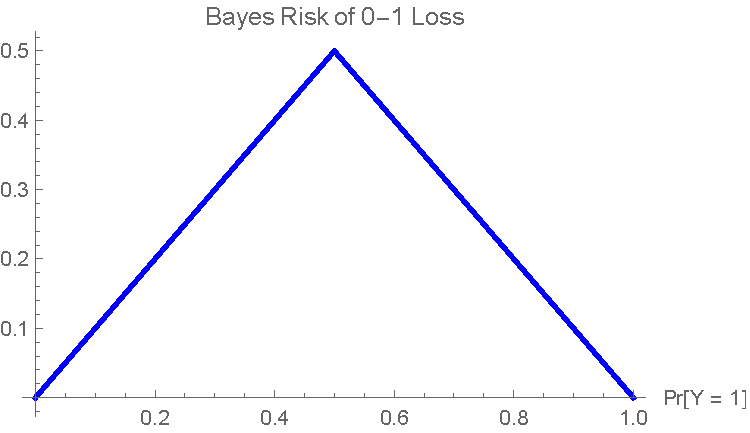
\includegraphics[width=0.95\linewidth]{figs/0-1-br.pdf}
%		\caption{Bayes risk of the 0-1 loss.}
%		\label{fig:0-1-br}
	\end{minipage}
	\hfill
	\begin{minipage}{0.3\linewidth}
	\centering		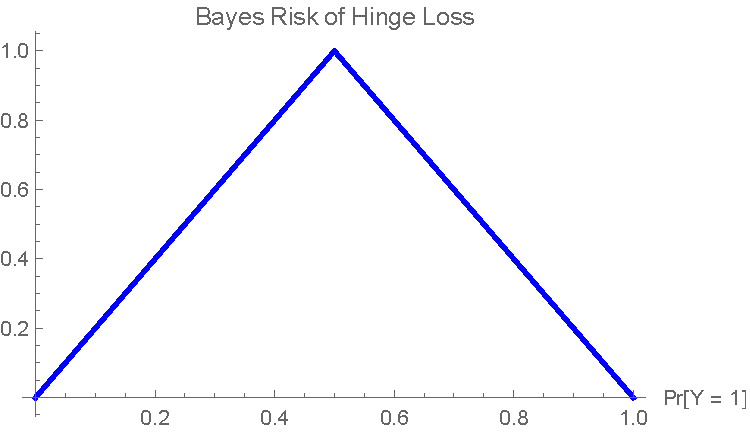
\includegraphics[width=0.95\linewidth]{figs/hinge-br.pdf}
%		\caption{Bayes risk of hinge loss.}
%		\label{fig:hinge-br}
	\end{minipage}
	\hfill
	\begin{minipage}{0.3\linewidth}
	\centering
	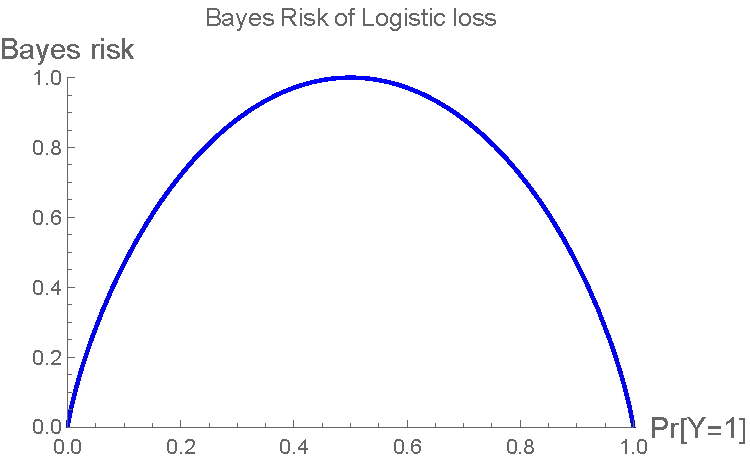
\includegraphics[width=0.95\linewidth]{figs/logistic-br.pdf}
%	\caption{Bayes risk of the logistic loss.}
%	\label{fig:logistic-br}
\end{minipage}
\caption{Bayes risks of 0-1, hinge, and logistic losses, respectively, in binary classification setting.}
\label{fig:bayes-risks-01}
\end{figure}

In this particular example, it is known $(\hinge,\psi)$ is calibrated for $\psi(u) = \sgn(u)$.
More generally, however, it is not clear whether an arbitrary embedding yields a calibrated link.
Indeed, apart from mapping the embedded points back to their original reports via $\psi(\varphi(r)) = r$, how to map the remaining values is far from obvious.
When the surrogate is polyhedral, we give a construction to map the remaining values in \S~\ref{sec:calibration}, showing that embeddings always yield calibration.
We first explore the connection between embeddings and polyhedral surrogates.


% Taking $\R = \{-1,1\}$ and the above embedding, we can write the expected loss over each report
% \begin{center}
% 	\begin{tabular}{ll}
% 		$\inprod{p}{\ellzo(1)} = (1-p_1)$ & $\inprod{p}{\ellzo(-1)} = (p_1)$\\
% 		$\inprod{p}{L_{hinge}(1)} = 2(1-p_1)$ & $\inprod{p}{L_{hinge}(-1)} = 2(p_1)$
% 	\end{tabular}
% \end{center}
% Thus, for every $r \in \R$ and $p \in \simplex$, we have $2 \inprod{p}{\ellzo(r)} = \inprod{p}{L_{hinge}(\varphi(r))}$.
% This leads us into the next section, where we show the Bayes Risks of the losses will be the same, accounting for the multiplicative constant, if one loss embeds the other.

% Additionally, one can see logistic loss does not embed $\ellzo$ because it elicits a continuous property, so there is an infinite set of unique optima over $\simplex$, and thus no injection exists mapping this set to $\{-1,1\}$.

% \raf{$L_{logistic}(u,y) := \ln\left(1 + \exp(-yu)\right)$}




% In another example, we consider the abstain loss and an embedding given by Ramaswamy et al.~\cite{ramaswamy2018consistent} in Section~\ref{sec:applications}, but note that the link function they provide is not unique.
% Essentially, the discrete abstain$(1/2)$ loss is minimized in expectation by predicting the most likely outcome $\argmax_y p_y$, conditioned on $p_y \geq 1/2$.
% If the most likely outcome is not likely enough, the loss is minimized by ``abstaining'' from predicting; a situation one can imagine would be useful if a false positive is costly.





\section{Embeddings and Polyhedral Losses}
\label{sec:poly-loss-embed}

In this section, we establish a tight relationship between the technique of embedding and the use of polyhedral (piecewise-linear convex) surrogate losses.
We defer the question of when such surrogates are consistent to \S~\ref{sec:calibration}. 
Throughout this section, unless specified otherwise, we use $\ell:\R\to\reals^\Y$ for discrete target losses and $L:\reals^d\to\reals^\Y$ for surrogates.

In Proposition~\ref{prop:embed-bayes-risks}, we show an equivalent condition to embedding, whose proof relies on the following Lemma about the Bayes risk of a ``restricted'' surrogate, shown here.
\begin{lemma}\label{lem:loss-restrict}
  Let $L$ elicit $\Gamma:\simplex\toto\R_1$, and let $\R_2\subseteq\R_1$ be representative for $L$.
  % such that $\Gamma(p) \cap \R_2 \neq \emptyset$ for all $p\in\simplex$.
  Then $L|_{\R_2}$ elicits $\gamma:\simplex\toto\R_2$ defined by $\gamma(p) = \Gamma(p)\cap \R_2$.
  Moreover, $\risk{L}=\risk{L|_{\R_2}}$.
\end{lemma}
\begin{proof}
	Let $p\in\simplex$ be fixed throughout.
	First let $r \in \gamma(p) = \Gamma(p) \cap \R_2$.
	Then $r \in \Gamma(p) = \argmin_{u\in\R_1} \inprod{p}{L(u)}$, so as $r\in\R_2$ we have in particular $r \in \argmin_{u\in\R_2} \inprod{p}{L(u)}$.
	For the other direction, suppose $r \in \argmin_{u\in\R_2} \inprod{p}{L(u)}$.
	By our assumption, we must have some $r^* \in \Gamma(p) \cap \R_2$.
	On the one hand, $r^*\in\Gamma(p) = \argmin_{u\in\R_1} \inprod{p}{L(u)}$.
	On the other, as $r^* \in \R_2$, we certainly have $r^* \in \argmin_{u\in\R_2} \inprod{p}{L(u)}$.
	But now we must have $\inprod{p}{L(r)} = \inprod{p}{L(r^*)}$, and thus $r \in \argmin_{u\in\R_1} \inprod{p}{L(u)} = \Gamma(p)$ as well.
	We now see $r \in \Gamma(p) \cap \R_2$.
	Finally, the equality of the Bayes risks $\min_{u\in\R_1} \inprod{p}{L(u)} = \min_{u\in\R_2} \inprod{p}{L(u)}$ follows immediately by the above, as $\emptyset \neq \Gamma(p)\cap\R_2 \subseteq \Gamma(p)$ for all $p\in\simplex$.
\end{proof}


%\jessiet{Make Construction- not definition}
%\begin{definition}[$\Sc(L)$]\label{cons:rep-set}
%	Suppose a generic loss $L : \R \to \reals^\Y$ is given with polyhedral negative risk $-\risk{L}$.
%	Construct the set $\Sc(L)$ as follows:
%	Each facet $F$ of the epigraph of negative risk $E_L$ must be full dimensional by definition of a facet.
%	Take $p \in \inter{F}$, and observe that it must by uniquely supported by some hyperplane $p \mapsto (p, L(u))$ for some $u \in \R$.
%	Add $u$ to $\Sc(L)$, and repeat, iterating over each of $E_L$'s finitely many facets.
%\end{definition}

\begin{proposition}\label{prop:SL-minimum}
  A loss $L: \R \to \reals^\Y_+$ has a polyhedral Bayes risk if and only if it has a finite representive set.
  % Moreover, for any minimum representative set $\Sc$ for $L$, there is a bijection between $\Sc$ and the facets of the epigraph of $-\risk{L}$.
  % \raft{Jessie: prove :-].  Note: min rep $\implies$ poly risk is immediate from Lemma~\ref{lem:loss-restrict}.  Move the construction into the proof. \jessie{Done; ready for a look}}
\end{proposition}
\begin{proof}
  A finite representative implies a polyhedral Bayes risk by Lemma~\ref{lem:loss-restrict}.
  
  For the converse, suppose $L$ has a polyhedral Bayes risk $\risk{L}$.
  Then we may write $\risk{L}(p) = \min_{(a,b)}$
  
  Let $\F$ be the set of facets of the epigraph of the negative Bayes risk

  implies it has a finite minimum representative set, we construct the set $\Sc$ as follows:

  since the epigraph of negative Bayes risk $E_L$ is polyhedral, it has finitely many facets, and we iterate over these.
  Each facet $F$ of $E_L$ must be full dimensional by definition of a facet, and therefore there must be some $p \in \inter{F}$.
  Observe that $p$ must by uniquely supported by some hyperplane $p \mapsto (p, L(u))$ for some $u \in \R$, since it is in the interior of the facet (and therefore $\risk{L}$ is differentiable at $p$).
  Add $u$ to $\Sc$, and repeat, iterating over each of $E_L$'s finitely many facets.
  We now show $\Sc$ is a minimum representative set.
  
  First, we have to show that $\Sc$ is a representative set.
  As facets are closed, for each facet $F$ and $p_F \in F$, there is a report $u_F \in \Sc$ by construction and closedness of facets so that the hyperplane $p_F \mapsto (p_F, \inprod{p_F}{L(u_F)})$ supports $E_L$ exactly on the facet. Therefore $u_F \in \Gamma(p) \cap \Sc$ for all $p$ such that the hyperplane supports $E_L$ at $p$.
  Representativeness follows as the facets of $E_L$ union to the simplex.
  
  If $\Sc$ was not a \emph{minimum} representative set \jessiet{minimal proof, not minimum}, then we could remove some $s$ from $\Sc$ such that $\Sc' := \Sc \setminus \{s\}$ is also a representative set for $L$.
  By the construction of $\Sc$ over facets of $E_L$, this report $s$ corresponds to a facet $F$ of $E_L$ since facets are full-dimensional and thus have well-defined nonempty interiors.
  There is then some distribution $p_F \in \inter F$ such that the hyperplane $p \mapsto (p, L(s))$ uniquely supports $E_L$ at $p_F$.
  We claim $\Gamma(p) \cap \Sc' = \emptyset$, since any other element $s'$ of $\Sc'$ being in $\Gamma(p)$ would imply $p \mapsto (p, L(s'))$ also supports $E_L$, but this hyperplane supporting $E_L$ must be unique, so these are equal.
  By construction of $\Sc$, we must have only added at most one of these to the set.
  Therefore, $\Sc$ is a minimum representative set.
  
  Moreover, we know there is a bijection between $\Sc$ and the facets of $E_L$ since $\card(\Sc) = |\Sc| = |\{F \mid F$ facet of $E_L\}| = \card($facets of $E_L)$ by construction of $\Sc$.
\end{proof}




To begin, we observe that our embedding condition in Definition~\ref{def:loss-embed} is equivalent to merely matching Bayes risks.
% For example, one can check that $\risk{\hinge} = 2\min\{p_1,p_2\} = 2\risk{\ellzo}$.
This useful fact will drive many of our results.


\begin{proposition}\label{prop:embed-bayes-risks}
  Let discrete loss $\ell$ be given.
  Then $L$ embeds $\ell$ if and only if $\risk{L}=\risk{\ell}$.
  % Let discrete loss $\ell:\R\to\reals^Y$ be given.
  % Then $L:\reals^d\to\reals^\Y$ embeds $\ell$ if and only if $\risk{L}=\risk{\ell}$.
  % A loss $L$ embeds a discrete loss $\ell$ if and only if $\risk{L}=\risk{\ell}$.
\end{proposition}
\begin{proof}
  \raft{4/2/2021 first part of the proof should be done now.}
  Define $\Gamma = \prop{L}$ and $\gamma = \prop{\ell}$.
  Suppose $L$ embeds $\ell$, so we have some $\Sc\subseteq \R$ which is representative for $\ell$ and an embedding $\varphi:\Sc\to\reals^d$; take $\U := \varphi(\Sc)$.
  Since $\Sc$ is representative for $\ell$, by embedding condition (ii) we have $\{\gamma_s \mid s\in\Sc\} = \{\Gamma_u \mid u\in\U\}$, so $\U$ is representative for $L$.
  % for all $p\in\simplex$ we have some $r \in \Sc \cap \gamma(p)$ and thus we have $\varphi(r) \in \U \cap \Gamma(p)$.
  % In particular, $\U \cap \Gamma(p)\neq \emptyset$ for all $p\in\simplex$, 
  By Lemma~\ref{lem:loss-restrict}, we have $\risk{\ell} = \risk{\ell|_{\Sc}}$ and $\risk{L} = \risk{L|_{\U}}$.
  % \raft{Commented out: the symmetric argument that representation goes both ways under an embedding.  I'm thinking we should expand on this perspective in section 5, maybe introduce a notion of equivalence between any two losses (discrete or otherwise), and define trim in that context.}
  % Taking $\U := \varphi(\Sc)$, we have that $\ell$ if and only if $\U$ is representative of $L$, as $\gamma(p) \cap \Sc \neq \emptyset \iff \exists r \in \Sc$ such that $r \in \gamma(p) \iff \exists r$ such that $\varphi(r) \in \Gamma(p) \cap \U \iff \Gamma(p) \cap \U \neq \emptyset$.
%  To see that $\gamma'(p) \neq \emptyset$ for all $p\in\simplex$, note that by the definition of $\gamma$ as the property elicited by $\ell$ we have some $r \in \gamma(p)$, and by the embedding condition~\eqref{eq:embed-loss}, $\varphi(r) \in \Gamma(p)$.
  As $L(\varphi(\cdot)) = \ell(\cdot)$ by embedding condition (i), for all $p\in\simplex$ we have
  \begin{equation*}
    \risk{\ell}(p) = \risk{\ell|_\Sc}(p) = \min_{r \in \Sc}\inprod{p}{\ell(r)} = \min_{r \in \Sc}\inprod{p}{L(\varphi(r))} = \min_{u \in \U}\inprod{p}{L(u)} = \risk{L|_\U}(p) = \risk{L}(p)~.
  \end{equation*}
  
    %\btw{RF: This is on the informal side, mostly because of the ``working in the affine hull'' bit.  It can all be formalized though, probably should be for the journal version: just take an appropriate linear projection of $\reals^n$ to $\reals^{n-1}$, and work with the projected versions of everything, and then project back.}
    
% commented out 10 May 21 to consolidate/clean/switch to proof relying on supporting hyperplanes of Bayes Risks
%    \jessie{Skip and go to orange for now.}
%  For the reverse implication, assume that $\risk{L} = \risk{\ell}$.
%  In what follows, we implicitly work in the affine hull of $\simplex$ by taking an appropriate invertible linear projection to an affine subspace $A : \reals^n_+ \to \reals^{n-1}_+$, so that interiors are well-defined, and $\risk{\ell}$ may be differentiable on the interior of $\simplex$.
%  (For intuition, one can consider the relative interiors in $\reals^\Y_+$, but we need to consider interiors in order to apply previous results.)
%  Since $\ell$ is discrete, $-\risk{\ell}$ is polyhedral as the pointwise maximum of a finite set of linear functions.
%  \raft{I believe we can remove mentions of power diagrams here; let's give it a try.  I don't think we need to project yet, given what we say next.}
%  The projection of its epigraph $E_{\ell}$ onto $\simplex$ forms a power diagram by Theorem~\ref{thm:aurenhammer}, whose cells are full-dimensional (in $n-1$ dimensions) and correspond to the level sets $\gamma_r$ of $\gamma = \prop{\ell}$. \jessiet{Don't need Theorem 1; can use Lemma~\ref{lem:finite-full-dim} instead. -21 Mar 21}

% commented out 10 May to consolidate/clean
%  \raft{Good start.  Let's take it a bit slower.  I was thinking you start with the facets, which by definition have interiors.  Then pick a point *of the graph*, one on the interior of each facet.  Then observe it must come from some $r$ and $p$, i.e., $(p,\inprod{p}{\ell(r)})$.  Now you can define $S$ (all the $r$'s you just gathered).  The embedding comes next, using the Bayes risk matching to get that same graph point written as $(p,\inprod{p}{L(u)})$: define $\varphi(r) = u$ for that $r$ and $u$.  And so on.}
%  \proposedadd{Take $S$ as follows: for each facet $F$ (of which there are finitely many) of the epigraph of $\ell$, $E_{\ell}$, there is at least one $r \in \R$ such that $(p, \inprod{p}{\ell(r)})$ supports $E_\ell$ on the facet $F$.
%  Form $S$ by taking one such report for each facet.}
%  For each $r\in\R\proposedadd{S}$, let $p_r$ be a distribution in the interior of $\gamma_r$, and let $u_r \in \Gamma(p)$.
%  Observe that, by definition of the Bayes risk and $\Gamma$, for all $v\in\reals^d$ the hyperplane $v \mapsto \inprod{v}{-L(u_r)}$ supports the epigraph $E_L$ of $-\risk{L}$ at the point $(p,-\inprod{p}{L(v)})$ if and only if $v\in\Gamma(p)$.
%  Thus, the hyperplane $v \mapsto \inprod{v}{-L(u_r)}$ supports $E_L = E_\ell$ at the point $(p_r,-\inprod{p_r}{L(u_r)})$, and thus does so at the entire facet $\{(p,-\inprod{p}{L(u_r)}) : p\in\gamma_r\}$; by the above, $u_r \in \Gamma(p)$ for all such distributions as well.
%  We conclude that $u_r \in \Gamma(p) \iff p \in \gamma_r \iff r \in \gamma(p)$, satisfying condition~\eqref{eq:embed-loss} for $\varphi : r \mapsto u_r$.
%  To see that the loss values match, we merely note that the supporting hyperplanes to the facets of $E_L$ and $E_\ell$ are the same, and the loss values are uniquely determined by the supporting hyperplane.
%  In particular, if $h$ supports the facet corresponding to $\gamma_r$, we have $\ell(r)_y = L(u_r)_y = h(\delta_y)$, where $\delta_y$ is the point distribution on outcome $y$.

	\jessiet{Not sure how much this matters, but technically, the $\Sc$ here might be different from the $\Sc$ in the forward implication, and might even be different cardinalities. Not sure if we want to change the notation to reflect this, or if that would just add confusion.}
	For the reverse implication, assume $\risk{L} = \risk{\ell}$, which are polyhedral functions as $\ell$ is discrete.  
	Construct a minimum representative set $\Sc$ via a bijection from the facets of $E_\ell$ as in the proof of Proposition~\ref{prop:SL-minimum}, and $\U$ similarly from $E_L$, with the embedding $\varphi : r \mapsto u_r$ if the hyperplanes $p \mapsto (p, \inprod{p}{\ell(r)})$ and $p \mapsto (p, \inprod{p}{L(u_r)})$ are equal.
	Such an embedding is well-defined as it is the composition of the bijections from reports in $\Sc$ and $\U$ to facets.
	%Since $\risk{\ell}$ is polyhedral, the epigraph of its negation, $E_\ell$, has a finite set of facets, which by definition have well-defined interiors.  For each facet, there must then be some distribution $p_r$ and report $r \in \R$ such that the hyperplane $p_r \mapsto (p_r, \inprod{p_r}{-\ell(r)})$ uniquely supports $E_\ell$.  Form $\Sc$ from the set of such reports $r$, iterating over each facet.  We have $\Sc$ representative for $\ell$ since the union of projected epigraph facets equals the simplex, and these facets and their projections are closed. Therefore, every $p \in \simplex$ is contained in some facet of the epigraph, and thus there is some $r \in \Sc$ so that $r \in \gamma(p)$.
%As the risks are equal, the same is true for $E_L$, e.g., for each facet, there is some $u_r$ so that $p_r \mapsto (p_r, \inprod{p_r}{L(u_r)})$, and one can construct the embedding $\varphi: r \mapsto u_r$ for each $r \in \Sc$.


We match optimality of embedded reports by construction, since the optimal reports support the epigraph of negative Bayes risk on exactly the same distributions, meaning a report and its embedding are optimal at exactly the same distributions.
To verify matching losses, consider that the hyperplanes $p \mapsto (p, \inprod{p}{\ell(r)})$ and $p \mapsto (p, \inprod{p}{L(\varphi(r))})$ are exactly equal since they are linear functions matching on a set of positive measure relative to the simplex, and must be equal everywhere.
This implies $\ell(r) = L(\varphi(r))$ for all $r \in \Sc$ such that the hyperplanes support $E_\ell$ and $E_L$ on a facet.
Since $\Sc$ and $\U$ are minimum representative sets, this holds for all $r \in \Sc$.
%To verify matching losses, observe $\risk \ell (\delta_y) = \risk L (\delta_y)$ for each $y \in \Y$, and these risks are attained by some report $r$ and its embedding $u_r$, respectively.
%\jessie{This feels like it's missing a detail about how $\Sc$ is minimum and how level sets are full-dimensional.}
\end{proof}

\raf{Something like this:}\\
Together, Lemma~\ref{lem:loss-restrict} and Proposition~\ref{prop:embed-bayes-risks} give the following useful tool for finding embeddings.
\begin{corollary}\label{cor:representative-embeds-restriction}
  Let surrogate loss $L:\reals^d \to \reals^\Y_+$ be given.
  If a finite set $\U \subseteq \reals^d$ is representative for $L$, then $L$ embeds the discrete loss $L|_\U$.\jessie{Type check: $\reals^d$ vs $\R$?}
\end{corollary}

%\btw{RF: matching risks is not necessary for \emph{consistency}, as evidenced by logistic loss for 0-1 loss.  Maybe we should just make the observation, earlier on, that \emph{embedding} is not necessary for consistency. \jessie{Added a few sentences above, when talking about consistency vs calibration.}}

%\btw{RF: DKR (section 3.1) realized the importance of matching Bayes risks, but they could only give general results for strictly convex (concave I should say) risks, in part because they fixed the link function to be a generalization of $\sgn$.  In contrast, we focus exclusively on non-strictly-convex risks.}



\raft{I wonder if we should demote this to a corollary.  We can write the proof of the reverse implication in Proposition~\ref{prop:embed-bayes-risks} like this: first show that if $\risk{L}$ is polyhedral, there is a finite $\U$ which is representative for $L$.  Then show that if $\risk{\ell} = \risk{L}$ then there is some $\Sc$ that is bijective to the particular $\U$ we constructed.  I'm not sure how this will go, but perhaps worth a try, since it would avoid the proof duplication too!}
\begin{proposition}\label{prop:embed-risk-poly}
  A loss $L$ embeds a discrete loss $\ell : \R \to \reals^\Y_+$ if and only if $\risk{L}$ is polyhedral.
\end{proposition}
\begin{proof}
  If $L$ embeds a discrete $\ell$, Proposition~\ref{prop:embed-bayes-risks} gives us $\risk{L} = \risk{\ell}$ and polyhedral.
  For the converse, let $\risk{L}$ be polyhedral. %; we again examine the proof of Proposition~\ref{prop:embed-bayes-risks}.
  Form the finite set $\Sc$ as the proof of Proposition~\ref{prop:SL-minimum}.
  %For each facet of $E_L$, which is full-dimensional, there must be some interior distribution $p$ such that $p \mapsto (p, \inprod{p}{L(u)})$ uniquely supports $E_L$, and such a $u$ must exist or else the Bayes risk is not attained.  Take $\Sc$ to be the collection of such reports $u$, and observe $\Sc$ is representative for $L$.  
  By Corollary~\ref{cor:representative-embeds-restriction}, $L$ embeds $L|_\Sc$, which is finite by construction.
%  The projection of the epigraph of $\risk{L}$ onto $\simplex$ forms a power diagram by Theorem~\ref{thm:aurenhammer} with finitely many cells $C_1,\ldots,C_k$, which we can index by $\R := \{1,\ldots,k\}$.
%  Defining the property $\gamma:\simplex\toto\R$ by $\gamma_r = C_r$ for $r\in\R$, we see that the same construction gives us points $u_r \in\reals^d$ such that $u_r \in \Gamma(p) \iff r \in \gamma(p)$.
%  Define $\ell:\R\to\reals^\Y_+$ by $\ell(r) = L(u_r)$, the same proof shows that $L$ embeds $\ell$.
\end{proof}



Shifting our focus to \emph{polyhedral} (piecewise linear and convex) surrogates, we observe that these surrogates elicit finite properties, though they may have optimal sets that are infinite.
This lets us apply results about finite representative sets to understand the structure of polyhedral surrogates and the losses they embed.
See \S~\ref{app:power-diagrams} for the full proof.

\begin{restatable}{lemma}{polyhedralrangegamma}
	\label{lem:polyhedral-range-gamma}
	Let $L:\reals^d\to\reals_+^\Y$ be a polyhedral loss, and let $\Gamma = \prop{L}$.
	Then the range of $\Gamma$, $\U = \Gamma(\simplex) = \{\Gamma(p) \subseteq \reals^d : p\in\simplex\}$, is a finite set of closed polyhedra.
        \raft{Leave this statement and add a proof sketch; move other dependencies to appendix \jessie{Done feel free to burn}}
\end{restatable}
\begin{proof}[Sketch]
	With $\Y$ finite, there are only finitely many supporting sets over $\simplex$.
	For $p \in \simplex$, the power diagram induced by projecting the epigraph of expected loss onto $\reals^d$ is the same for any $p$ of the same support (Lemma~\ref{lem:polyhedral-pd-same}).
	Moreover, we have $\Gamma(p)$ being exactly one of the faces of the projected epigraph since the hyperplane $u \mapsto (u, \inprod{p}{L(u)})$ supports the epigraph of the expected loss at exactly the property value.
	Since this epigraph has finitely many faces, the range of $\Gamma$ is then (a subset) of elements of a finitely generated (finite supports) set of finite elements (finite faces).
\end{proof}

This insight lets us delve further into understanding characteristics of polyhedral surrogates.

\begin{lemma}
	\label{lem:poly-loss-poly-risk}
	If $L$ is polyhedral, $\risk{L}$ is polyhedral.
\end{lemma}
\begin{proof}
	Let $L:\reals^d\to\reals_+^\Y$ be a polyhedral loss, and $\Gamma = \prop{L}$.
	By Lemma~\ref{lem:polyhedral-range-gamma}, $\U = \Gamma(\simplex)$ is finite. 
	For each $U\in \U$, select $u_U \in U$, and let $\Sc = \{u_U : U \in\U\}$.
	$\Sc$ is representative for $L$, so Lemma~\ref{lem:loss-restrict} gives us $\risk{L} = \risk{L|_{\Sc}}$, which is polyhedral as $\Sc$ is finite.
\end{proof}

From the more succinct embedding condition in Proposition~\ref{prop:embed-risk-poly}, we can in turn simplify the condition that a loss embeds \emph{some} discrete loss: it does if and only if its Bayes risk is polyhedral.
(We say a concave function is polyhedral if its negation is a polyhedral convex function.)
Note that the Bayes risk, a function from distributions over $\Y$ to the reals, may be polyhedral even if the loss itself is not.
For example, this can be seen by a loss that is polyhedral in the convex hull of $\varphi(\R)$, but smooth outside that region.

Previous work from~\citet[Proposition 4]{duchi2018multiclass} realized the significance of matching Bayes risks for calibration with respect to the 0-1 loss, but their result relies the Bayes risk of the surrogate being strictly concave.  As polyhedral functions are never strictly concave, Proposition~\ref{prop:embed-risk-poly} extends their result to the embedding setting.


Combining Proposition~\ref{prop:embed-risk-poly} with the observation that polyhedral losses have polyhedral Bayes risks (Lemma~\ref{lem:poly-loss-poly-risk}), we obtain the first direction of our equivalence between polyhedral losses and embedding.

\begin{theorem}\label{thm:poly-embeds-discrete}
  Every polyhedral loss $L$ embeds a discrete loss.
\end{theorem}

We now turn to the reverse direction: which discrete losses are embedded by some polyhedral loss?
Perhaps surprisingly, we show that \emph{every} discrete loss is embeddable,
using a construction via convex conjugate duality which has appeared several times in the literature (e.g.\ \cite{duchi2018multiclass,abernethy2013efficient,frongillo2014general}).
Note however that the number of dimensions $d$ required could be as large as $O(|\Y|)$, which is particularly undesirable in structured prediction and information retrieval problems with exponentially many outcomes.
Recent work~\citep{ramaswamy2016convex,finocchiaro2020embedding,finocchiaro2021unifying} yield characterizations for bounding the prediction dimension $d$ for consistent convex surrogates and embeddings.
%\raft{CITE: DKR, frongillo-kash (WINE 2014), probably one of Bob's papers?, others?}

\begin{theorem}\label{thm:discrete-loss-poly-embeddable}
  Every discrete loss $\ell:\R \to \reals^\Y_+$ is embedded by a polyhedral loss.
\end{theorem}
\begin{proof}
  Let $n = |\Y|$, and let $C:\reals^n \to \reals$ be given by $(-\risk{\ell})^*$, the convex conjugate of $-\risk{\ell}$.
  From standard results in convex analysis, $C$ is polyhedral as $-\risk{\ell}$ is, and $C$ is finite on all of $\reals^\Y$ as the domain of $-\risk{\ell}$ is bounded~\cite[Corollary 13.3.1]{rockafellar1997convex}.
  Note that $-\risk{\ell}$ is a closed convex function, as the infimum of affine functions, and thus $(-\risk{\ell})^{**} = -\risk{\ell}$.
  Define $L:\reals^n\to\reals^\Y$ by $L(u) = C(u)\ones - u$, where $\ones\in\reals^\Y$ is the all-ones vector.
  As $C$ is polyhedral, so is $L$.
  We first show that $L$ embeds $\ell$, and then establish that the range of $L$ is in fact $\reals^\Y_+$, as desired.

  We compute Bayes risks and apply Proposition~\ref{prop:embed-bayes-risks} to see that $L$ embeds $\ell$.
  Observe that $\risk{\ell}$ is polyhedral as $\ell$ is discrete.
  For any $p\in\simplex$, we have
  \begin{align*}
    \risk{L}(p)
    &= \inf_{u\in\reals^n} \inprod{p}{C(u)\ones - u}\\
    &= \inf_{u\in\reals^n} C(u) - \inprod{p}{u}\\
    &= -\sup_{u\in\reals^n} \inprod{p}{u} - C(u)\\
    &= -C^*(p) = - (-\risk{\ell}(p))^{**} = \risk{\ell}(p)~.
  \end{align*}
  It remains to show $L(u)_y \geq 0$ for all $u\in\reals^n$, $y\in\Y$.
  Letting $\delta_y\in\simplex$ be the point distribution on outcome $y\in\Y$, we have for all $u\in\reals^n$, $L(u)_y \geq \inf_{u'\in\reals^n} L(u')_y = \risk{L}(\delta_y) = \risk{\ell}(\delta_y) \geq 0$, where the final inequality follows from the nonnegativity of $\ell$.
  \btw{FUTURE: to get $n-1$, just use the same trick as before and note that the Bayes risk doesn't change.  Should be a couple lines.}
\end{proof}

\proposedadd{Moreover, to construct an embedding of dimension $n-1$ instead of $n$ (see~\citet{finocchiaro2020embedding} for significance of dimension),  consider some invertible linear transformation $A : \reals^n \to \reals^{n-1}$ that maps to an affine subspace.
Take $L' : \reals^{n-1} \to \reals^\Y$ as $x \mapsto L(A^{-1}(x))$ and $L$ defined as above, so that $\inprod{\ell(r)}{p} = \inprod{L(\varphi(r))}{p} = \inprod{L'(A^{-1}(\varphi(r)))}{p} $ for all $p \in \simplex$.
The Bayes risks $\risk{L}(p)$ and $\risk{L'}(p)$ are equal for all $p \in \simplex$; thus, the result holds in $n-1$ dimensions as well.}\jessiet{Leaving this change in the macro for proofreading.}

%\btw{Cut summary for now (Why is this cool?)}
%\jessiet{Jessie: added a bit to say why this is cool.}
We will see that embedding implies the existence of a consistent surrogate and link, so this result tells us that, for discrete losses, the embedding framework is sufficient to understand the existence of consistent surrogates for the given loss.
Even if there is a smooth surrogate for a given discrete loss, there is also a polyhedral loss that is calibrated for the given loss.
What's more is that there is a polyhedral \emph{embedding} that is calibrated for the discrete loss.


%\begin{corollary}\label{cor:finite-elicit-embed}
%  Let $\gamma$ be a finite property.
%  The following are equivalent.
%  \begin{enumerate}\setlength{\itemsep}{0pt}
%  \item $\gamma$ is elicitable.
%  \item $\gamma$ is embeddable.
%  \item $\gamma$ is embeddable via a polyhedral loss.
%  \end{enumerate}
%\end{corollary}
%\begin{proof}
%  We trivially have $3\Rightarrow 2$.
%  The direction $1\Rightarrow 3$ follows from Theorem~\ref{thm:discrete-loss-poly-embeddable}, by taking any discrete loss which elicits $\gamma$.
%  Finally, to see $2\Rightarrow 1$,
%  \raf{This follows from Proposition~\ref{prop:embed-trim}, but we're stating this as a corollary... let's see if it follows more directly from the above.  If it doesn't (one complication: there is no discrete loss starting from $2$ or $3$!) we can rephrase it as a theorem / proposition.}
%\end{proof}


\section{Consistency via Calibrated Links}
\label{sec:calibration}

We have now seen the tight relationship between polyhedral losses and embeddings; in particular, every polyhedral loss embeds some discrete loss.
The embedding itself tells us how to link the embedded points back to the discrete reports (map $\varphi(r)$ to $r$), but it is not clear when this link can be extended to the remaining reports, and whether such a link can lead to consistency.
In this section, we give a construction to generate calibrated links for \emph{any} polyhedral loss.

\S~\ref{app:calibration} contains the full proof; this section provides a sketch along with the main construction and result.
The first step is to give a link $\psi$ such that exactly minimizing expected surrogate loss $L$, followed by applying $\psi$, always exactly minimizes expected original loss $\ell$.
The existence of such a link is somewhat subtle, because in general some point $u$ that is far from any embedding point can minimize expected loss for two very different distributions $p,p'$, making it unclear whether there exists a choice $\psi(u)\in\R$ that is $\ell$-optimal for both distributions.
We show that as we vary $p$ over $\simplex$, there are only finitely many sets of the form $U = \argmin_{u \in \reals^d} \inprod{p}{L(u)}$ (Lemma~\ref{lem:polyhedral-range-gamma}).
Associating each $U$ with $R_U \subseteq \R$, the set of reports whose embedding points are in $U$, we enforce that all points in $U$ link to some report in $R_U$.
(As a special case, embedding points must link to their corresponding reports.)
Proving that these choices are well-defined uses a chain of arguments involving the Bayes risk, ultimately showing that if $u$ lies in multiple such sets $U$, the corresponding report sets $R_U$ all intersect at some $r =: \psi(u)$.

%
%\begin{proposition}\label{prop:embed-link}
%  Let $L$ elicit $\Gamma:\simplex\toto\reals^d$ which embeds a finite property $\gamma$.
%  Then there exists a link function $\psi: \reals^d \to \R$ that is \emph{valid} in the sense that, for any $p$, if $u$ minimizes expected $L$-loss (i.e. $u \in \Gamma(p)$, then $\psi(u)$ minimizes expected $\ell$-loss (i.e. $\psi(u) \in \gamma(p)$).
%\end{proposition}
%\begin{proof}
%  Let $\gamma:\simplex\toto\R$.
%  Proposition~\ref{prop:embed-trim} gives us that $\trim(\Gamma) = \{\gamma_r : r\in\R\}$.
%  \bo{Have we defined trim already? Or is this proof going to the appendix?}
%  Then for any $u\in\reals^d$, there is some $r\in\R$ such that $\Gamma_u \subseteq \gamma_r$.
%  The link $\psi : \reals^d \to \R$ which encodes these choices is valid.
%\end{proof}

Intuitively, to ensure calibration, we just need to ``thicken'' this construction, by mapping all approximately-optimal points $u$ to optimal reports $r$.
Let $\U$ contain all optimal report sets $U$ of the form above.
A key step in the following definition will be to narrow down a ``link envelope'' $\Psi$ where $\Psi(u)$ denotes the legal or valid choices for $\psi(u)$.

%\begin{lemma}
%  \label{lem:polyhedral-range-gamma}
%  Let $L:\reals^d\to\reals_+^\Y$ be a polyhedral loss, and let $\Gamma = \prop{L}$.
%  Then the range of $\Gamma$, $\U = \Gamma(\simplex) = \{\Gamma(p) \subseteq \reals^d | p\in\simplex\}$, is a finite set of closed polyhedra.
%\end{lemma}
%For each of these finitely many $U \in \U$, we let $R_U$ be the set of reports whose embedding points lie in $U$.
%The idea will be to map points in $U$, as well as points nearby, to something in $R_U$
%We show in the full version \bo{okay wording?} that for any $p$, if $U = \Gamma(p)$, then $R_U = \gamma(p)$.

\begin{definition} \label{def:eps-thick-link}
  Given a polyhedral $L$ that embeds some $\ell$, an $\epsilon > 0$, and a norm $\|\cdot\|$, the \emph{$\epsilon$-thickened link} $\psi$ is constructed as follows.
  First, initialize $\Psi: \reals^d \toto \R$ by setting $\Psi(u) = \R$ for all $u$.
  Then for each $U \in \U$, for all points $u$ such that $\inf_{u^* \in U} \|u^*-u\| < \epsilon$, update $\Psi(u) = \Psi(u) \cap R_U$.
  Finally, define $\psi(u) \in \Psi(u)$, breaking ties arbitrarily.
  If $\Psi(u)$ became empty, then leave $\psi(u)$ undefined.
\end{definition}

\btw{JOURNAL: cool to point out that when $L$ is polyhedral, $\prop{L}$ has a finite range (this result) and so does its (multivalued map) inverse (trim result)!}

% \begin{proposition}
%   If $\psi$ is a separated link between losses $L$ and $\ell$, then $L$ and $\psi$ are consistent with respect to $\ell$. \jessie{Rephrase?}
% \end{proposition}
% \begin{proof}
%   \raf{Use Hari's theorems from their section 8.}
% \end{proof}

\begin{theorem}\label{thm:eps-thick-calibrated}
  Let $L$ be polyhedral, and $\ell$ the discrete loss it embeds from Theorem~\ref{thm:poly-embeds-discrete}.
  Then for small enough $\epsilon > 0$, the $\epsilon$-thickened link $\psi$ is well-defined and, furthermore, is a calibrated link from $L$ to $\ell$.
\end{theorem}

\begin{proof}[Sketch]
  \emph{Well-defined:}
  For the initial construction above, we argued that if some collection such as $U,U',U''$ overlap at a $u$, then their report sets $R_U, R_{U'}, R_{U''}$ also overlap, so there is a valid choice $r = \psi(u)$.
  Now, we thicken all sets $U \in \U$ by a small enough $\epsilon$; it can be shown that if the \emph{thickened} sets overlap at $u$, then $U,U',U''$ themselves overlap, so again $R_U, R_{U'}, R_{U''}$ overlap and there is a valid chioce $r = \psi(u)$.

  \emph{Calibrated:} By construction of the thickened link, if $u$ maps to an incorrect report, i.e.\ $\psi(u) \not\in \gamma(p)$, then $u$ must have at least distance $\epsilon$ to the optimal set $U$.
  We then show that the minimal gradient of the expected loss along any direction away from $U$ is lower-bounded, giving a constant excess expected loss at $u$.
\end{proof}

\btw{FUTURE: we should comment in the discussion section that we probably can show that *any* loss embedding $\ell$ must be polyhedral-ish, meaning polyhedral except for stuff that is never optimal.  This theorem would then not need the ``polyhedral'' part. This is related to the ``convex envelope conjucture'', that if $L$ embeds $\ell$ via $\varphi$, you can just take the loss $L'$ such that $L_y$ is the convex envelope of points $\{(\varphi(r),L(r)_y)\}_{r\in\R}$.}
\btw{FUTURE: This prop and theorem give an excellent reason to focus on embeddings, since other techniques do not necessarily give you separated links for free.  Since we know we get them for free, we can just focus on the property, and study elicitation complexity; we know if we have a link at all it can be taken to be separated.  [[Is this true?]]}



Note that the construction given above in Definition~\ref{def:eps-thick-link} is not necessarily computationally efficient as the number of labels $n$ grows.
In practice this potential inefficiency is not typically a concern, as the family of losses typically has some closed form expression in terms of $n$, and thus the construction can proceed at the symbolic level.
We illustrate this formulaic approach in \S~\ref{sec:abstain}.
% \proposedadd{In general, we are not overly concerned with the computational complexity of computing the surrogate and link, since these calculations only need to be computed once.  They are generally derived mathematically, rather than computationally.  These symbolic calculations typically tend to be straightforward, but can sometimes be tricky.}



%%%%%%%%%%%%%%%%%%%%%%%%%%%%%%%%%%%%%%%%%%%%%%%%%%%%%%%%%%%%%%%
\section{Application to Specific Surrogates}\label{sec:applications}

Our results give a framework to construct consistent surrogates and link functions for any discrete loss, but they also provide a way to verify the consistency or inconsistency of given surrogates.
Below, we illustrate the power of this framework with specific examples from the literature, as well as new examples.
In some cases we simplify existing proofs, while in others we give new results, such as a new calibrated link for abstain loss, and the inconsistency of the recently proposed Lov\'asz hinge.
\btw{RF: The top-k and hypercube/set examples (except abstain) have the link built in, e.g.\ as the sign function), and they just work around it.  Our results may suggest that it's worth thinking ``outside the box'' (HAH, genious...) and looking for embeddings which are not the hypercube. \jessie{Added a bit discussing this, starting at ``the examples in ...''.}}
The examples in \S~\ref{sec:applications}, with the exception of the abstain surrogate given by~\citet{ramaswamy2018consistent}, all present a surrogate that use the link $\psi: u \mapsto \sgn(u)$.
While this may sometimes yield a calibrated link, this is not always the case.
In fact, we will see that most of these examples do not yield calibrated surrogates, although proving that there is \emph{no} calibrated link for a given surrogate is quite difficult.
Our results suggest that it is possible that some of the given surrogates are calibrated, but perhaps one must use a nontraditional link in order to calibrate the loss, such as the thickening construction given here.
\citet{wang2020weston} apply the embedding framework to show that the Weston-Watkins hinge loss embeds a discrete loss for ordered partitions.


\subsection{Consistency of abstain surrogate and link construction}
\label{sec:abstain}

In classification settings with a large number of labels, several authors consider a variant of classification, with the addition of a ``reject'' or \emph{abstain} option.
For example, \citet{ramaswamy2018consistent} study the loss $\ellabs{\alpha} : [n] \cup \{\bot\} \to \reals^\Y_+$ defined by $\ellabs{\alpha}(r)_y = 0$ if $r=y$, $\alpha$ if $r = \bot$, and 1 otherwise.
%\begin{align}\label{eq:abstain-discrete}
%$\ellabs{\alpha}(r)_y = \begin{cases}
%0 & r = y\\
%\alpha & r = \bot\\
%1 & \text{otherwise}
%\end{cases}~.$
%\end{align}
Here, the report $\bot$ corresponds to ``abstaining'' if no label is sufficiently likely, specifically, if no $y\in\Y$ has $p_y \geq 1-\alpha$.
\citet{ramaswamy2018consistent} provide a polyhedral surrogate for $\ellabs{\alpha}$, which we present here for $\alpha=1/2$.
Letting $d = \ceil{\log_2(n)}$ their surrogate is $L_{1/2} : \reals^d \to \reals^\Y_+$ given by
\begin{equation}\label{eq:abstain-surrogate}
L_{1/2}(u)_y = \left(\max\nolimits_{j \in [d]}B(y)_j u_j + 1\right)_+~,
\end{equation}
where $B:[n]\to\{-1,1\}^d$ is a arbitrary injection; let us assume $n = 2^d$ so that we have a bijection.
Consistency is proven for the following link function,
\begin{equation}\label{eq:abstain-link}
  \psi(u) = \begin{cases}
	\bot & \min_{i \in [d]} |u_i| \leq 1/2\\
	B^{-1}(\sgn(-u)) &\text{otherwise}
  \end{cases}~.
\end{equation}

In light of our framework, we can see that $L_{1/2}$ is an excellent example of an embedding, where $\varphi(y) = B(y)$ and $\varphi(\bot) = 0 \in \reals^d$.
Moreover, the link function $\psi$ can be recovered from Theorem~\ref{thm:eps-thick-calibrated} with norm $\|\cdot\|_\infty$ and $\epsilon=1/2$; see Figure~\ref{fig:abstain-links}(L).
Hence, our framework would have simplified the process of finding such a link, and the corresponding proof of consistency.
To illustrate this point further, we give an alternate link $\psi_1$ corresponding to $\|\cdot\|_1$ and $\epsilon=1$, shown in Figure~\ref{fig:abstain-links}(R):
\begin{equation}\label{eq:abstain-link-1}
  \psi_1(u) = \begin{cases}
	\bot & \|u\|_1 \leq 1\\
	B^{-1}(\sgn(-u)) &\text{otherwise}
  \end{cases}~.
\end{equation}
Theorem~\ref{thm:eps-thick-calibrated} immediately gives calibration of $(L_{1/2},\psi_1)$ with respect to $\ellabs{1/2}$.
Aside from its simplicity, one possible advantage of $\psi_1$ is that it appears to yield the same constant in generalization bounds as $\psi$, yet assigns $\bot$ to much less of the surrogate space $\reals^d$.
It would be interesting to compare the two links in practice.

The embedding framework can also be applied to understand the hierarchical extension of the BEP surrogate given by~\citet{ramaswamy2015hierarchical}, who present a convex, calibrated surrogate for the hierarchical classification problem.
Given a tree $H = ([n], E,W)$ over finite class labels, they consider the discrete loss 
\begin{equation}\label{eq:tree-loss-discrete}
	\ell^H(r,y) = \text{shortest path length in $H$ between $r$ and $y$}
\end{equation}
They generalize the BEP embedding to this problem and show their extension is consistent with respect to eq.~\eqref{eq:tree-loss-discrete}; we can also verify this is an embedding and subsume their result through Theorem~\ref{thm:poly-ie-implies-consistent}.


\begin{figure}
\begin{center}
\begin{minipage}{0.32\linewidth}
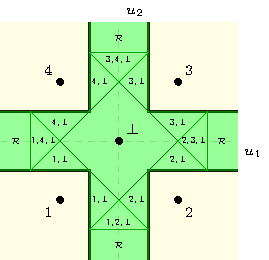
\includegraphics[width=\linewidth]{tikz/abstain-link-linf.pdf}
\end{minipage}\hfill
\begin{minipage}{0.32\linewidth}
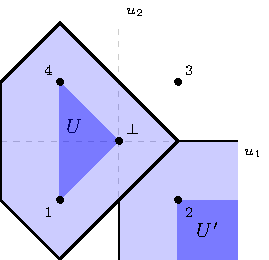
\includegraphics[width=\linewidth]{tikz/abstain-link-U-regions-l1.pdf}
\end{minipage}\hfill
\begin{minipage}{0.32\linewidth}
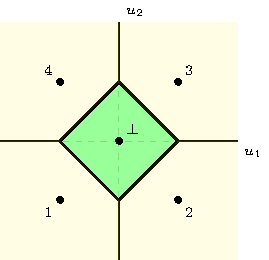
\includegraphics[width=\linewidth]{tikz/abstain-link-l1.pdf}
\end{minipage}\hfill
\caption{Constructing links for the abstain surrogate $L_{1/2}$ with $d=2$. The embedding is shown in bold labeled by the corresponding reports. (L) The link envelope $\Psi$ resulting from Theorem~\ref{thm:eps-thick-calibrated} using $\|\cdot\|_\infty$ and $\epsilon = 1/2$, and a possible link $\psi$ which matches eq.~\eqref{eq:abstain-link} from~\cite{ramaswamy2018consistent}.  (M) An illustration of the thickened sets from Definition~\ref{def:eps-thick-link} for two sets $U \in \U$, using $\|\cdot\|_1$ and $\epsilon = 1$. (R) The $\Psi$ and $\psi$ from Theorem~\ref{thm:eps-thick-calibrated} using $\|\cdot\|_1$ and $\epsilon = 1$.}
\label{fig:abstain-links}
\end{center}
\end{figure}


\subsection{Inconsistency of Lov\'asz hinge}
\label{sec:lovasz-hinge}

Many structured prediction settings can be thought of as making multiple predictions at once, with a loss function that jointly measures error based on the relationship between these predictions~\cite{hazan2010direct, gao2011consistency, osokin2017structured}.
In the case of $k$ binary predictions, these settings are typically formalized by taking the predictions and outcomes to be $\pm 1$ vectors, so $\R=\Y=\{-1,1\}^k$.
One then defines a joint loss function, which is often merely a function of the set of mispredictions, meaning we may write $\ell^g(r)_y = g(\{i \in [k] : r_i \neq y_i\})$ for some set function $g:2^{[k]}\to\reals$.
For example, Hamming loss is given by $g(S) = |S|$.
In an effort to provide a general convex surrogate for these settings when $g$ is a submodular function, Yu and Blaschko~\cite{yu2018lovasz} introduce the \emph{Lov\'asz hinge}, which leverages the well-known convex Lov\'asz extension of submodular functions.
While the authors provide theoretical justification and experiments, consistency of the Lov\'asz hinge is left open, which we resolve.

Rather than formally define the Lov\'asz hinge, we defer the complete analysis to the full version of the paper~\cite{finocchiaro2019embedding}, and focus here on the $k=2$ case.
For brevity, we write $g_\emptyset := g(\emptyset)$, $g_{1,2} := g(\{1,2\})$, etc.
%\raft{Jessie: I meant \emph{our} paper :-].  Leaving this here:\cite{yu2015lovaszarxiv}}
Assuming $g$ is normalized and increasing (meaning $g_{1,2} \geq \{g_1,g_2\} \geq g_\emptyset = 0$), the Lov\'asz hinge $L:\reals^k\to\reals^\Y_+$ is given by
\begin{multline}
  \label{eq:lovasz-hinge}
  L^g(u)_y = \max\Bigl\{(1-u_1y_1)_+ g_1 + (1-u_2y_2)_+ (g_{1,2}-g_1),\\[-4pt] (1-u_2y_2)_+ g_2 + (1-u_1y_1)_+ (g_{1,2}-g_2)\Bigr\}~,
\end{multline}
where $(x)_+ = \max\{x,0\}$.
We will explore the range of values of $g$ for which $L^g$ is consistent, where the link function $\psi:\reals^2\to\{-1,1\}^2$ is fixed as $\psi(u)_i = \sgn(u_i)$, with ties broken arbitrarily.

Let us consider the coefficients $g_\emptyset = 0$, $g_1 = g_2 = g_{1,2} = 1$, for which $\ell^g$ is merely 0-1 loss on $\Y$.
For consistency, for any distribution $p\in\simplex$, we must have that whenever $u \in \argmin_{u'\in\reals^2} \inprod{p}{L^g(u')}$, the outcome $\psi(u)$ must be the most likely, i.e., in $\argmax_{y\in\Y} p(y)$.
Simplifying eq.~\eqref{eq:lovasz-hinge}, however, we have
\begin{equation}
  \label{eq:lovasz-hinge-abstain}
  L^g(u)_y = \max\bigl\{(1-u_1y_1)_+,(1-u_2y_2)_+\bigr\} = \max\bigl\{1-u_1y_1,1-u_2y_2,0\bigr\}~,
\end{equation}
which is exactly the abstain surrogate~\eqref{eq:abstain-surrogate} for $d=2$.
We immediately conclude that $L^g$ cannot be consistent with $\ell^g$, as the origin will be the unique optimal report for $L^g$ under distributions with $p_y < 0.5$ for all $y$, and one can simply take a distribution which disagrees with the way ties are broken in $\psi$.
For example, if we take $\sgn(0) = 1$, then under $p((1,1)) = p((1,-1)) = p((-1,1)) = 0.2$ and $p((-1,-1)) = 0.4$, we have $\{0\} = \argmin_{u\in\reals^2} \inprod{p}{L^g(u)}$, yet we also have $\psi(0) = (1,1) \notin \{(-1,-1)\} = \argmin_{r\in\R} \inprod{p}{\ell^g(r)}$.

In fact, this example is typical: using our embedding framework, and characterizing when $0\in\reals^2$ is an embedded point, one can show that $L^g$ is consistent if and only if $g_{1,2} = g_1 + g_2$.
Moreover, in this linear case, which corresponds to $g$ being \emph{modular}, the Lov\'asz hinge reduces to weighted Hamming loss, which is trivially consistent from the consistency of hinge loss for 0-1 loss.
In the full version of the paper~\cite{finocchiaro2019embedding}, we generalize this observation for all $k$: $L^g$ is consistent if and only if $g$ is modular.
In other words, even for $k>2$, the only consistent Lov\'asz hinge is weighted Hamming loss.
These results cast doubt on the effectiveness of the Lov\'asz hinge in practice.


% \subsection{New surrogates for cost-sensitive classification}

% \raf{I think we should cut this subsection, and maybe just remind the reader at the prelude to this section that Theorem~\ref{thm:discrete-loss-poly-embeddable} gives a construction for any discrete loss.}
% The construction given in Theorem~\ref{thm:discrete-loss-poly-embeddable}, together with the calibrated link construction in Section~\ref{sec:calibration}, can generate consistent convex surrogates for arbitrary discrete losses.
% For example, consider cost-sensitive classification; given an arbitrary loss matrix $C \in \reals^{n\times n}_+$ describing the loss $\ell_j(i) = C_{ij}$ of predicting label $i$ when the true label is $j$, we construct a convex surrogate based on the convex conjugate of $-\risk{\ell}$.
% While of course several surrogates are known for this problem~\cite{pires2013cost}, they typically work in $n$ dimensions.
% %\raf{Jessie, could you cite \url{http://proceedings.mlr.press/v28/avilapires13.pdf} here}
% one advantage of our embedding framework is the ability to construct lower-dimensional surrogates when costs have certain geometric interpretations.
% For example, if $v_1,\ldots,v_n \in \reals^k$ are on the unit sphere and $C_{ij} = \inprod{v_i}{v_j}$, we can simply take $L_j(u) = $\raf{aaaand Noah woke up}\raf{Just realized that this loss matrix has rank $k$ and thus is covered by AA15: just elicit the linear property $\E v_Y \in \reals^k$.}

\subsection{Inconsistency of top-$k$ losses}
% 7.14.19- proposed version for arXiv
%\jessiet{The story we discussed: YK show $L'$ is inconsistent.  Our framework lets us ask: with what discrete loss \emph{is} $L'$ consistent?  (It also assures us that $L'$ is consistent for something...) Oh look, $L'$ embeds something which is $\elltopk$ plus some other term, so (a) we can see very clearly what $L'$ ``is doing'', and (b) we can see where to look for distributions yielding inconsistency, namely ones for which we actually prefer to report a set with $|r|<k$.}

% As one instance, the top-$k$ classification problem is to predict the set of $k$ most likely labels; formally, we have $\R := \{r \subseteq [n] : |r| = k\}$, $\Y = [n]$, 
% $1<k<n$, and discrete loss $\elltopk : r \mapsto \Ind{y \not\in r}$.
In certain classification problems when ground truth may be ambiguous, such as object identification, it is common to predict a set of possible labels.
As one instance, the top-$k$ classification problem is to predict the set of $k$ most likely labels; formally, we have $\R := \{r \in \{0,1\}^n : \|r\|_0 = k\}$, $1<k<n$, $\Y = [n]$, and discrete loss $\elltopk(r)_y = 1-r_y$.
Surrogates for this problem commonly take reports $u\in\reals^n$, with the link $\psi(u) = \{u_{[1]},\ldots,u_{[k]}\}$, where $u_{[i]}$ is the $i^{th}$ largest entry of $u$.
% , with ties broken arbitrarily.

\citet{lapin2015top, lapin2016loss, lapin2018analysis} provide the following convex surrogate loss for this problem, which \citet{yang2018consistency} show to be inconsistent:%
\footnote{\citet{yang2018consistency} also introduce a consistent surrogate, but it is non-convex.}
\begin{align}\label{eq:L-2-surrogate}
L^k(u)_y := \left( 1-u_y + \tfrac{1}{k} \textstyle\sum_{i=1}^k (u - e_y)_{[i]} \right)_+~,
\end{align}
where $e_y$ is $1$ in component $y$ and 0 elsewhere.
With our framework, we can say more.
Specifically, while $(L^k,\psi)$ is not consistent for $\elltopk$, since $L^k$ is polyhedral (Lemma~\ref{lem:top-k-polyhedral}), we know from Theorem~\ref{thm:poly-embeds-discrete} that it embeds \emph{some} discrete loss $\ell^k$, and from Theorem~\ref{thm:eps-thick-calibrated} there is a link $\psi'$ such that $(L^k,\psi')$ is calibrated (and consistent) for $\ell^k$.
We therefore turn to deriving this discrete loss $\ell^k$.

For concreteness, consider the case with $k = 2$ over $n=3$ outcomes.
We can re-write $L^2(u)_y = \left(1 - u_y + \tfrac 1 2 (u_{[1]}+ u_{[2]} - \min(1,u_y))\right)_+$.
By inspection, we can derive the properties elicited by $\elltop{2}$ and $L^2$, respectively, which reveals that the set $\R'$ consisting of all permutations of $(1,0,0)$, $(1,1,0)$, and $(2,1,0)$, are always represented among the minimizers of $L^2$.
Thus, $L^2$ embeds the loss $\ell^2(r)_y = 0$ if $r_y = 2$ or $\ell^2(r)_y = 1 - r_y + \tfrac 1 2 \inprod{r}{\ones-e_y}$ otherwise.
Observe that $\ell^2$ is just $\elltop{2}$ with an extra term punishing weight on elements other than $y$, and a reward for a weight of 2 on $y$.

Moreover, we can visually inspect the corresponding properties (Fig.~\ref{fig:top-k-simplices}) to immediately see why $L^2$ is inconsistent: for distributions where the two least likely labels are roughly equally (un)likely, the minimizer will put all weight on the most likely label, and thus fail to distinguish the other two.
More generally, $L^2$ cannot be consistent because the property it embeds does not ``refine'' (subdivide) the top-$k$ property, so not just $\psi$, but \emph{no} link function, could make $L^2$ consistent.

\begin{figure}[H]
	\begin{minipage}{0.45\linewidth}
		\centering
		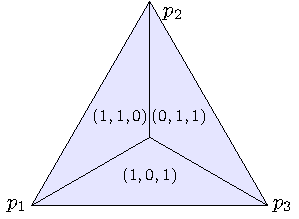
\includegraphics[width=\linewidth]{tikz/original-top-k}
		\label{fig:original-top-k}
	\end{minipage}
	\hfill
	\begin{minipage}{0.45\linewidth}
		\centering
		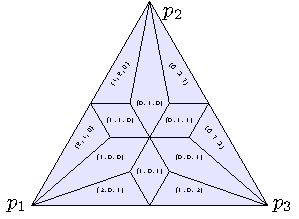
\includegraphics[width=\linewidth]{tikz/finite-surrogate-top-k}
		\label{fig:finite-surrogate-top-k}
	\end{minipage}
	\caption{Minimizers of $\inprod{p}{\elltop{2}}$ and $\inprod{p}{\ell^2}$, respectively, varying $p$ over $\Delta_3$.}
	\label{fig:top-k-simplices}
\end{figure}

\btw{Yutong's paper commented out here; mentioned at beginning of section- June 1 21}
%\subsection{Embedding Ordered Partitions}
%\citet*{wang2020weston} use embeddings to construct and prove the calibration of the Weston-Watkins surrogate for the \emph{Ordered Partition} loss.
%
%An ordered partition on $[n] := \{1, \ldots, n\}$ is an ordered list $S = (S_1, \ldots, S_l)$ of nonempty, pairwise disjoint sets such that $\cup_i S_i = [n]$, and assume $l \geq 2$.
%The ordered partition target loss $\ell^{\OP}$ is defined, for $i \in [n]$ and $S = (S_1, \ldots, S_l) \in \OP_n$ by
%\begin{align*}
%\ell^\OP(S,y) &= |S_1| - 1 + \sum_{i=1}^{l-1} |S_1 \cup \ldots \cup S_{i+1}| \cdot \Ind{y \not \in S_1 \cup \ldots \cup S_i}~.~
%\end{align*}
%The summation in this ordered partition loss can be interpreted as a variation of 0-1 loss where one can report sets of sets, and increases the punishment for the outcome $y$ not being in the earlier sets in the ordering; outside the summation is a punishment for having a large prediction set on the first $S_1$.
%This work presents an embedding for $\ell^\OP$ and uses this fact to show that the Weston-Watkins hinge loss~\citep{weston1999support} is in fact calibrated (and hence consistent, since the two are equivalent in Quadrant 1) with respect to $\ell^\OP$.
%
%The Weston-Watkins hinge loss takes predictions $u \in \reals^n$ and assigns loss
%\begin{equation}\label{eq:ww-hinge}
%L(u,y) = \sum_{i \in \Y : i \neq y} (1 - (u_y - u_i))_+~.~
%\end{equation}
%
%\citet[Definition 2.3]{wang2020weston} takes the embedding $\varphi : \OP_n \to \reals^n$ entrywise so that for all $j \in S_i$, we have $\varphi(S)_j = -(i-1)$.
%
%\begin{figure}[H]
%		\centering
%		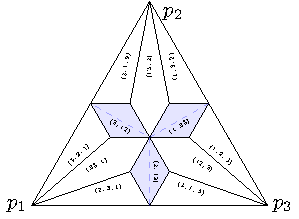
\includegraphics[width=0.5\linewidth]{tikz/ordered-partition}
%	\caption{Level sets of the Weston Watkins hinge with embedding given by~\citet[Definition 2.3]{wang2020weston}.}
%	\label{fig:ordered-partition}
%\end{figure}


\btw{Hierarchical surrogate commented out; just mention in 7.1 since it builds off of that example.}
%\subsection{Embedding hierarchical classifications}
%Our final example comes from \citet{ramaswamy2015hierarchical}, who present a convex, calibrated surrogate for the hierarchical classification problem.
%Given a tree $H = ([n], E,W)$ over finite class labels, they consider the discrete loss 
%\begin{equation}\label{eq:tree-loss-discrete}
%	\ell^H(r,y) = \text{shortest path length in $H$ between $r$ and $y$}
%\end{equation}
%In this setting, the outcomes $\Y$ are composed of all nodes in the tree and not just the leaves.
%
%\begin{figure}
%	\centering
%		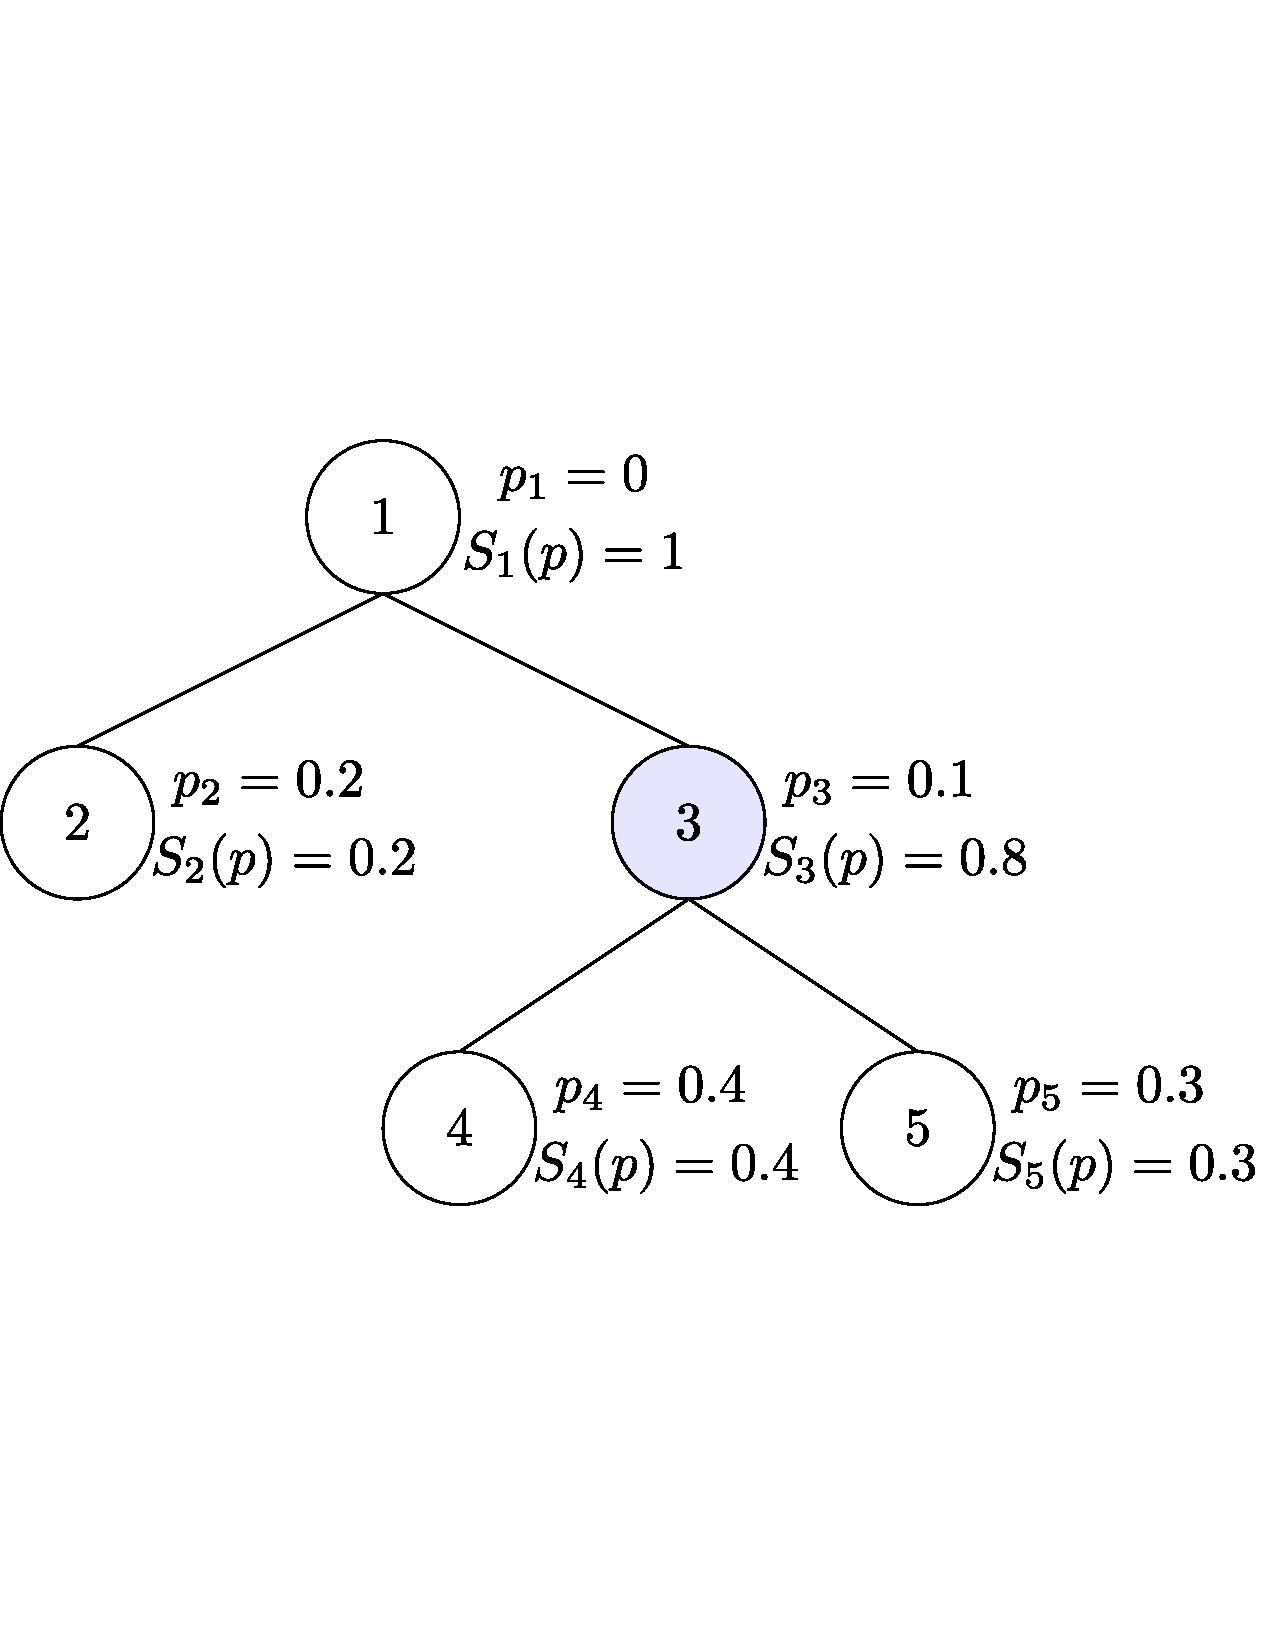
\includegraphics[width=0.7\linewidth]{tikz/example-tree-deeper.pdf}
%		\caption{Tree $H$ with distribution $\vec p = (0, .2, .1, .4, .3)$. $\gamma^H(\vec p) = 3$.}\label{fig:example-tree-deeper}
%\end{figure}
%
%
%\begin{figure}
%\begin{minipage}{0.45\linewidth}
%	\centering
%	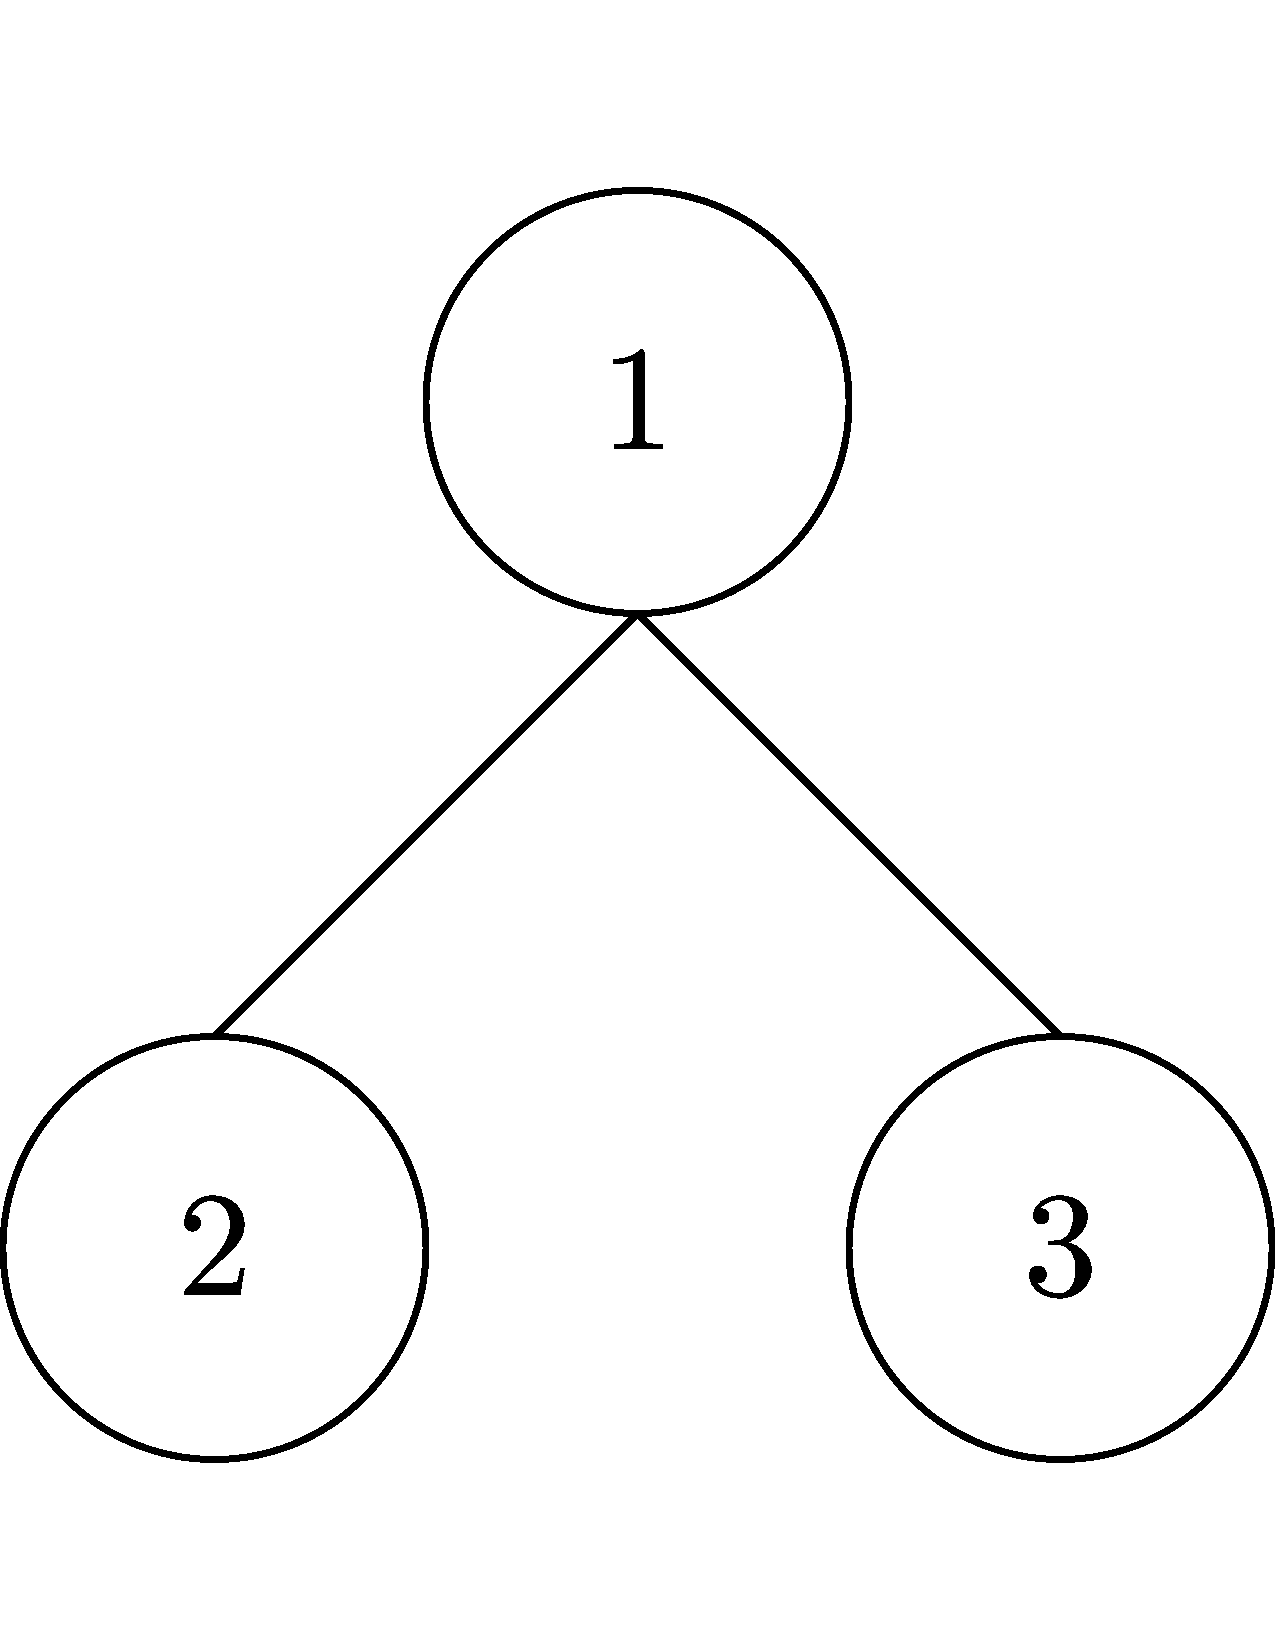
\includegraphics[width=0.9\linewidth]{tikz/3-node-tree.pdf}
%	\caption{3 node tree whose property we evaluate in next image.}
%	\label{fig:3-node-tree}
%\end{minipage}
%\hfill
%\begin{minipage}{0.45\linewidth}
%	\centering
%	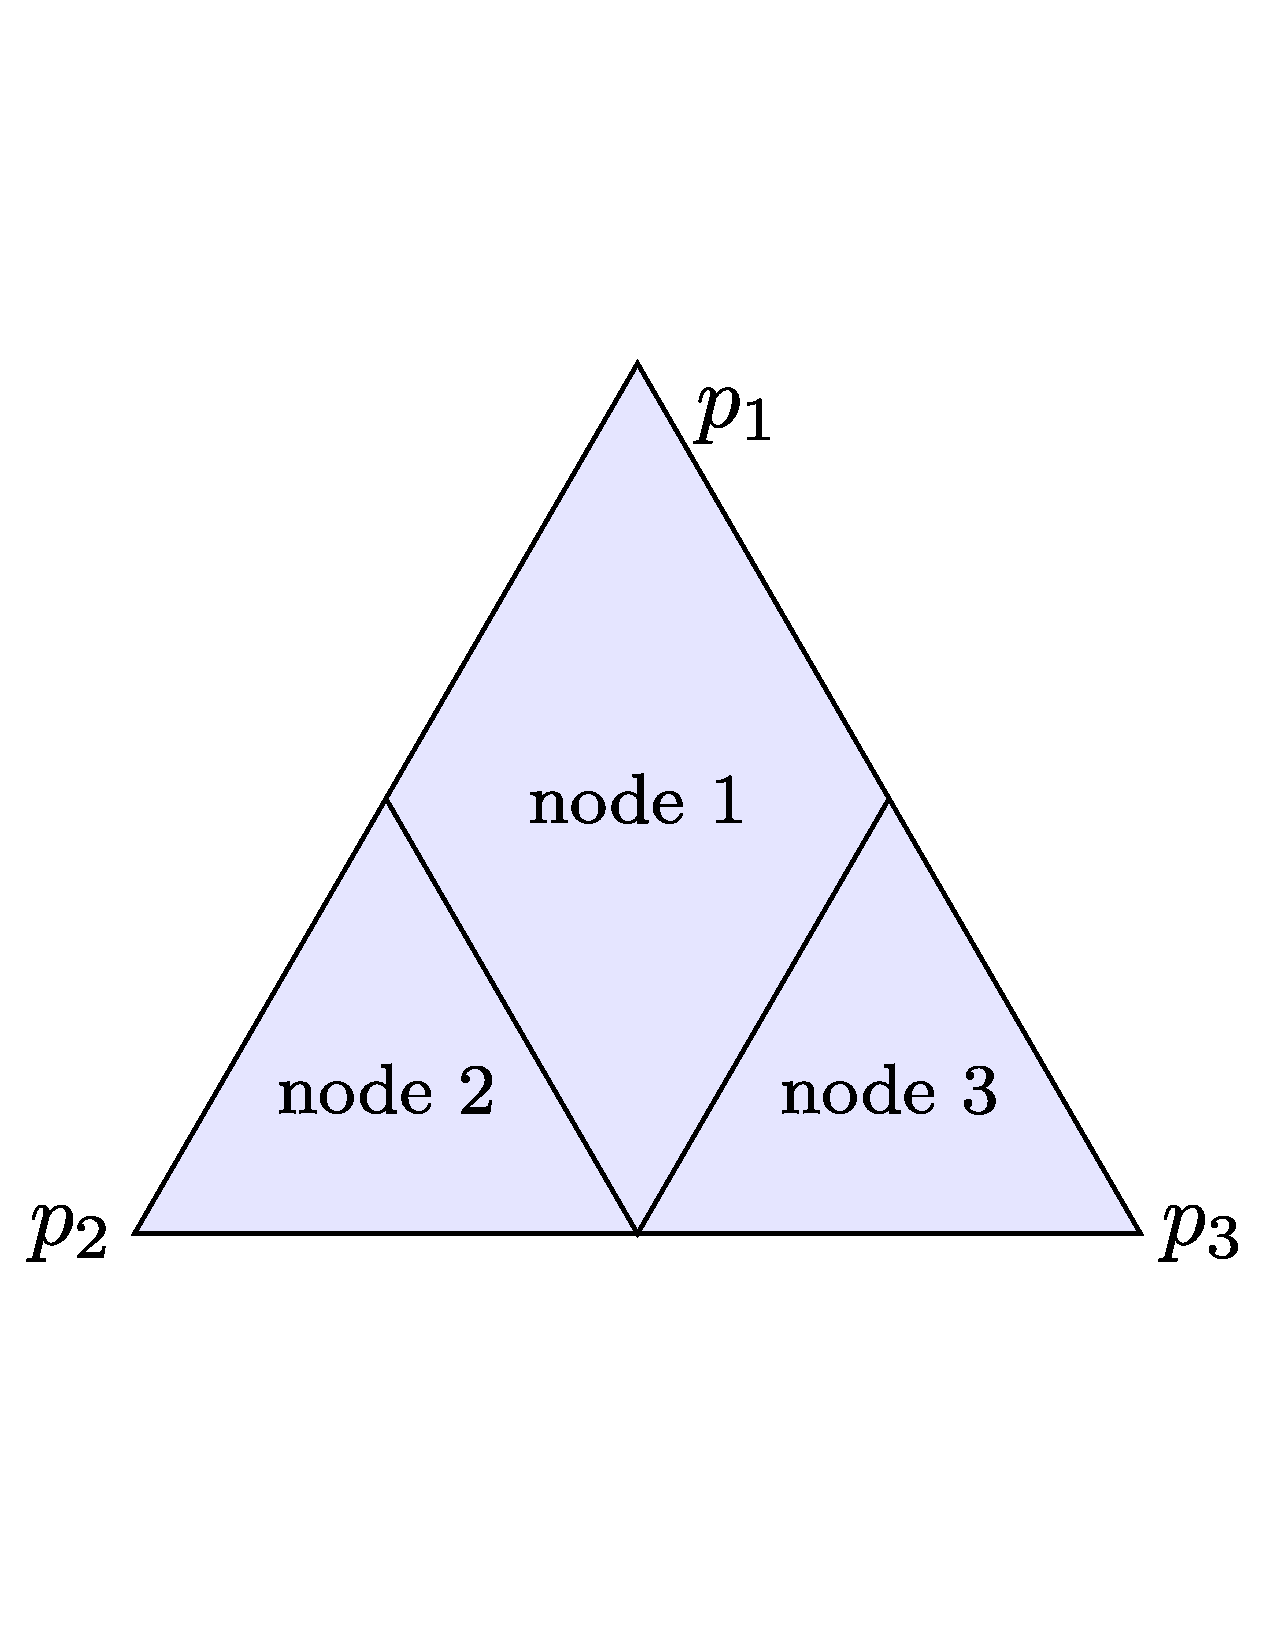
\includegraphics[width=0.9\linewidth]{tikz/3-node-tree-prop.pdf}
%	\caption{Property elicited by unweighted 3-node tree.}
%	\label{fig:3-node-tree-prop}
%\end{minipage}
%\end{figure}
%
%In~\cite[Theorem 1]{ramaswamy2015hierarchical}, Ramaswamy et al. show the property $\gamma^H := \prop{\ell^H}$ is the deepest node $i$ in the tree $H$ such that the probability that node $i$ or one of its descendants is the outcome, denoted $S_i(p)$, is greater than or equal to $1/2$.
%They additionally note that this property is agnostic to the weight $W$ of the tree.
%As before, consider $p_i$ to be the probability that node $i$ is the ground truth label, and $S_i(p)$ to be the probability that node $i$ or one of its descendants is the ground truth.
%For an example, see Figure~\ref{fig:example-tree-deeper}, where predicting node $3$ minimizes the expected tree loss over the distribution $\vec p = (0, 0.2, 0.1, 0.4, 0.3)$.
%
%Letting $h$ be the height of the tree $H$, Ramaswamy et al. present an embedding of $\ell^H$ that consists of learning $h$ $\abstain{1/2}$ embeddings, where the outcomes at the $j^{th}$ embedding are the nodes on level $j$ of the tree.
%At each highest level, one proceeds down the path of the tree given by the prediction of the current abstain embedding.
%If one predicts $\bot$ at level $j$, then we predict the node predicted at the $(j-1)^{st}$ level.
%
%Note that the given \emph{Cascade Surrogate} of~\citet[Equation 2]{ramaswamy2015hierarchical} simply requires the use of a surrogate that is calibrated with respect to $\abstain{1/2}$, so we can use the BEP surrogate of~\citet{ramaswamy2018consistent} to concatenate $h$ $\ceil{\log_2(n)}$ dimensional embeddings for the tree loss, yielding an embedding for $\ell^H$.
%
%It is worth noting that the cascade surrogate is not the always most efficient in terms of dimension.
%For example, the cascading surrogate on the 3 node tree $H$ in Figure~\ref{fig:3-node-tree} takes two $1$-dimensional optimization problems for distributions $p$ such that $p_1 < 1/2$.
%However, the property (Figure~\ref{fig:3-node-tree-prop}) elicited by tree distance for $H$ in Figure~\ref{fig:3-node-tree} is embeddable by a real-valued surrogate thanks to the characterization of \cite[\S~3]{finocchiaro2020embedding}, so one can see that the dimension cascade surrogate does not yield a tight bound.
%This leaves the question of embedding dimension open for the hierarchical surrogate embedding the discrete tree loss $\ell^H$.
%
%% \jessie{Don't think we need the below addition for the camera ready, but will eventually want something along these lines for the arXiv version.}
%% \proposedadd{To generalize this result, first consider that Lapin's surrogate is polyhedral, and we propose that each coordinate of an optimal report $u \in \reals_+^n$ must be at one of three points: $0$, $1$, or another ``high'' point that is a function of the number of high points and $M = |\{i : u_i = 1\}|$.  Since there are only a finite number of such optimal reports, $\R$, we know that this embeds a finite loss, namely $L^2_\R$.
%% \begin{align*}
%% \R := \left\{ \frac{|M| + k -1}{k - |H|} \mathbf{1}_H + \mathbf{1}_M : H, M \subset [n], H\cap M = \emptyset, |H| + |M| \leq k \right\}
%% \end{align*}
%% The discrete loss $\ell^{top-2} = L^2|_\R$ is then defined as follows:
%% \begin{equation}
%% \ell^{top-k}(r,y) = \begin{cases}
%% 0 & r_y = \bar r_{-y} + 1\\
%% \bar r - \frac 1 k & r_y = 1\\
%% 1 + \bar r & r_y = 0
%% \end{cases}~,~
%% \end{equation}
%% where $\bar r = \frac 1 k \sum_{i=1}^k r_{[i]}$.
%% }

%%%%%%%%%%%%%%%%%%%%%%%%%%%%%%%%%%%%%%%%%%%%%%%%%%%%%%%%%%%%%%%%%%%%%%
%% Jessie's version here 7/16/2019

% Figure~\ref{fig:top-k-simplices} (left) gives a map of the property values of $\gamma^{\text{top-2}} := \prop{\elltop{2}}$ over $\Delta_3$.
% Similarly, for every distribution $p \in \Delta_3$, $\inprod{p}{L^2}$ has a minimizer in the set $\R'$ composed of the tuples shown in Figure~\ref{fig:top-k-simplices} (right), and thus $\risk{L^2} = \risk{\ell^2}$, where $\ell^2 := L^2|_{\R'}$, so Figure~\ref{fig:top-k-simplices} (right) shows $\gamma^2 := \prop{\ell^2}$.
% %Therefore, we know $L^2$ embeds $\ell^2$ by Proposition~\ref{prop:embed-bayes-risks}.
% %(Each cell in this simplex is a level set $\gamma^{\text{top-2}}_r$ and corresponds to a flat piece of the Bayes Risk $\risk{\elltop{2}}$.)

% By visual inspection, we can observe there is no ``refining'' mapping from $\gamma^{\text{top-2}}$ to $\gamma^2$.
% In refining, we loosely mean that, for some $j \in \R$, there is no $I \subseteq \reals^n$ such that $\cup_{i \in I}\gamma^2_i = \gamma^{\text{top-2}}_{j}$.
% %If such a mapping existed, it would allude to one possible consistent link $\psi$ by which $L^2$ embeds $\elltop{2}$.
% Conversely, we can ``refine'' $\prop{L^2}$ down to $\prop{\ell^2}$ by using the axiom of choice to construct $\R'$.

% \jessie{Not sure if this is too much detail...}
% Since $\prop{\elltop{2}}$ does not refine $\prop{L^2}$, then $L^2$ does not embed $\elltop{2}$.
% For example, we can take distributions $p_1 \in \gamma^{top-2}_{\{1,2\}}$ and $p_2 \in \gamma^{top-2}_{\{1,3\}}$ such that $p_1, p_2 \in \Gamma_{(1,0,0)}$.
% Regardless of $\psi((1,0,0))$, for either $p_1$ or $p_2$, we will observe $\psi((1,0,0)) \not \in \argmin_u \inprod{p_i}{\elltop{2}(u)}$.
% Thus, we see that $L^2$ is not a consistent surrogate for $\elltop{2}$.


%%%%%%%%%%%%%%%%%%%%%%%%%%%%%% old version submitted to NuerIPS%%%%%%%%%%%%%%%%%%%%%%%%%%%%%%%%%%
%\btw{The story we discussed: YK show $L'$ is inconsistent.  Our framework lets us ask: with what discrete loss \emph{is} $L'$ consistent?  (It also assures us that $L'$ is consistent for something...) Oh look, $L'$ embeds something which is $\elltopk$ plus some other term, so (a) we can see very clearly what $L'$ ``is doing'', and (b) we can see where to look for distributions yielding inconsistency, namely ones for which we actually prefer to report a set with $|r|<k$.}
%
%In certain classification problems, for example in information retrieval, it is common to predict a set of possible labels.
%As one instance, for $k<n$ the top-$k$ classification problem has reports $\R := \{r \subseteq [n] : |r| = k\}$, with label $y \in [n]$.
%The natural discrete loss $\elltopk:\R \to \reals^\Y_+$ is given by
%\begin{align}\label{eq:top-k}
%  \elltopk(r,y) = \Ind{y \not \in r}~,
%\end{align}
%which simply gives a penalty if the label was not in the reported set.
%
%Surrogates for this problem commonly take reports $u\in\reals^n$, with the link $\psi(u) = \{u_{[1]},\ldots,u_{[k]}\}$, where $x_{[u]}$ is the $i^{th}$ largest component of $u$, with ties broken arbitrarily.
%\citet{lapin2015top, lapin2016loss, lapin2018analysis} provide the following convex surrogate loss for this problem, which \citet{yang2018consistency} show to be inconsistent:%
%\footnote{Yang and Koyejo also introduce a consistent surrogate, but it is non-convex.}
%\begin{align}\label{eq:L-2-surrogate}
%  L'(u)_y := \left( \tfrac{1}{k} \textstyle\sum_{i=1}^k (u + \ones - e_y)_{[i]} - u_y \right)_+~,
%\end{align}
%where $e_y$ is $1$ in component $y$ and 0 elsewhere.
%
%With our framework, we can say more.
%Specifically, while $(L',\psi)$ is not consistent for $\elltopk$, since $L'$ is polyhedral (Lemma~\ref{lem:top-k-polyhedral}), we know from Theorem~\ref{thm:poly-embeds-discrete} that it embeds \emph{some} discrete loss $\ell'$, and from Theorem~\ref{thm:eps-thick-calibrated} there is a link $\psi'$ such that $(L',\psi')$ is calibrated (and consistent) for $\ell'$.
%We therefore turn to deriving this discrete loss $\ell'$.
%
%In Lemma~\ref{lem:top-k-optimal-corners}\jessiet{in the Appendix... remove ref for camera ready version}, we show that the set $\U = \{u \in \{0,1\}^n : \|u\|_0 \leq k\}$ is always represented among the optimizers of $L'$, meaning for all $p \in \simplex$ we have $\prop{L'}(p) \cap \U \neq \emptyset$.
%From Lemma~\ref{lem:loss-restrict}\raft{was Lemma~\ref{lem:top-k-surrogate-embeds}}, then, $L'$ must embed $L'|_\U$, which gives us $\ell':\R'\to\reals^\Y_+$ via the natural embedding from sets $\R' = \{r \subseteq [n] : |r| \leq k\}$ to their indicator vectors:
%\begin{align}\label{eq:ell-2}
%\ell'(r)_y &= \Ind{y \not\in r} + \tfrac 1 k |r \setminus \{y\}| = (1+\tfrac 1 k)\Ind{y \not\in r} + \tfrac 1 k (|r|-1)~.
%\end{align}
%We now see that $\ell'$ is essentially $\elltopk$ (extended to sets smaller than $k$) plus an additional cardinality term which rewards smaller sets.
%
%Knowledge of what loss $L'$ actually embeds greatly simplifies the task of proving inconsistency with $\elltopk$.
%Specifically, we see that $\ell'$ allows sets of cardinality strictly less than $k$, so we can look for a distribution making one of these smaller sets optimal.
%Writing the expected loss, we have
%%$\inprod{p}{\ell'(r)} = 1 - p(r) + \tfrac 1 k (|r|-p(r)) = 1 + \tfrac 1 k |r| - (1 + \tfrac 1 k) p(r)$,\\
%$\inprod{p}{\ell'(r)} = (1+\tfrac 1 k)(1 - p(r)) + \tfrac 1 k (|r|-1) = 1 + \tfrac 1 k |r| - (1 + \tfrac 1 k) p(r)$, where $p(r) = \sum_{i\in r} p_i$.
%% It is now easy to see that the optimal $r$ for any fixed cardinality $|r|=c$ is the $c$ most likely labels.
%So let us ask when it is better to drop an element $i$ from $r$:
%% If $i$ is the index of the $c$th most likely label (so $p_i = p_{[c]}$)
%we have $\inprod{p}{\ell'(r)-\ell'(r\setminus\{i\})} = \tfrac 1 k - (1+\tfrac 1 k)p_i$, meaning we will drop elements from $r$ until they all have weight at least $\tfrac 1 {k+1}$.
%In particular, for distributions close to uniform, $r=\emptyset$ is optimal, already giving us inconsistency\raft{If space (nope) we should spell this out like Jessie did: however ties are broken at $u=0$, pick a distribution with bumps going against the ties, and $u=0$ is still optimal.}.
%More generally, as $k < n$, the set $P = \{p\in\simplex : \max_{r\in\R'} p(r) < k/(k+1)\}$ is full-dimensional and guarantees that at least one of the top $k$ labels has probability strictly less than $\tfrac 1 {k+1}$.
%
%% We now focus on the case where $k=1$; the top-$k$ loss reduces to 0-1 loss in this case.
%% To show a set of distributions where $\prop{\ell'}(p) \neq \prop{\elltopk}(p)$, we claim that $\vec{0}~\in~\prop{\ell'} \implies \risk{\ell'}(p) = 1$ for any $p$ with $\max_y p_y \leq 1/2$.
%% Additionally $\risk{\ell_{top-1}}(p) = 1 - \max_y p_y < 1 \implies \vec{0} \not\in \prop{\elltopk}(p)$.
%
%% First, $\ell(\vec{0}, \bar{p}) = 1$ for all $p \in \simplex$.
%% Taking the set $\{y\}$ for any $y \in \Y$, the expected loss $\inprod{p}{\ell'(\{y\})} = 2 (1-p_y) \geq 1$ by assumption on $p$.
%% %For any $r$ such that $|r| \geq 2$ \jessiet{In general, $|r| \geq k+1$}, we know that  $\ell'(r)_y \geq 1$ for all $y \in \Y$, so the expected loss much be greater than or equal to $1$.
%% Therefore, we have that $\vec{0} \in \prop{\ell'}(p)$ but $\vec{0} \not\in \prop{\elltopk}(p)$ for any $p$ such that $\max_y p_y \leq 1/2$.
%
%
%
%%Since we can see that $\ell' \neq \elltopk$, we can then see that $L'$ is not consistent with respect to $\elltopk$.
%%Similarly, given $L_4(u,y) := \max\left(\frac{1}{k} \sum_{i=1}^k (1 + u_{\setminus y})_{[i]} - s_y, 0\right)$, we can actually see that $L_4$ also embeds $\ell'$.
%%We will double up on notation and call this discrete loss $\ell_4$ as well, for the sake of matching subscripts of discrete losses to the surrogates that embed them.

%%%%%%%%%%%%%%%%%%%%%%%%%%%%%%%%%%%%%%%%%%%%%%%%%%%%%%%%%%%%%%%



%%%%%%%%%%%%%%%%%%%%%%%%%%%%%%%%%%%%%%%%%%%%%%%%%%%%%%%%%%%%%%%
\section{Minimum Representative Sets and Non-redundancy}
\label{sec:min-rep-sets}

% commented out 19 Apr 21
% \raf{Some thoughts on this section:
% \begin{itemize}
% \item It's unclear to me how much of the properties stuff is for funzies versus useful in the sense that it's clearer to dispense with the loss.
% \item It seems nice to point out and explore the fact that our notion of embedding is, now, symmetric.
%   \begin{itemize}
%   \item So generally we could say $L_1:\R_1\to\reals^\Y$ and $L_2:\R_2\to\reals^\Y$ are \emph{equivalent} (name TBD) if there exist $\Sc_i\subseteq\R_i$ representative for $L_i$, $i\in\{1,2\}$, with a bijection $\varphi:\Sc_1\to\Sc_2$ such that (i) for all $r\in\Sc_1$ we have $L_2(\varphi(r)) = L_1(r)$, and (ii) for all $p\in\simplex, r\in\R_1$ we have $r\in\prop{L_1}(p) \iff \varphi(r)\in\prop{L_2}(p)$.
%   \item Now since $\varphi$ is a bijection it's clear that this is an equivalence relation.
%   \item Moreover, since we've already established (Prop~\ref{prop:embed-bayes-risks}) that if $L$ embeds discrete $\ell$ over $\Sc$, then $\Sc$ being representative for $\ell$ implies $\varphi(\Sc)$ is representative for $L$, meaning $L$ and $\ell$ are equivalent under this definition.
%   \item What other results might hold more generally using this equivalence notion?  (Note: finiteness of $\Sc$ is not assumed now, though we could make that assumption.)
%   \item I believe the Bayes risk matching result may hold: $L_1$ and $L_2$ are equivalent iff $\risk{L_1}=\risk{L_2}$.  Certainly the first direction (equivalent $\implies$ risk matching) goes through untouched.  For the converse, I think we need finiteness of $\trim$, or maybe more generally some condition about the differentiability of the risk, since we needed the uniqueness of the supporting hyperplane to $\risk{L}$ to deduce that the losses matched.  Otherwise, if the Bayes risk has a nondifferentiable point, and the the level set of $u$ is that point, and $u$ is not redundant, there will be multiple loss vectors at $u$ which achieve the same Bayes risk.
%   \end{itemize}
% \end{itemize}}
% \jessie{Thinking about this: I think there is enough value to $\trim$ as an object to include it.  The concept makes a lot more intuitive sense if we defined it by $\trim_\Sc(\gamma) = \{\gamma_r : r \in \Sc\}$ and thinking about the importance of $\Sc$.
% There are a few results that are well-explained by this:
% \begin{itemize}
%	\item $L$ embeds discrete $\ell$ over set $\Sc$ (minimum representative for $\ell$) iff $\trim_\Sc(\prop{\ell}) = \trim_{\varphi(\Sc)}(\prop{L})$
%	\item $L$ is equivalent to discrete $\ell$ iff $\trim_{\R_1}(\prop{\ell}) = \trim_{\R_2}(\prop{L})$
%	\item when is $\ell$ non-redundant? (no reports $r$ s.t. $\gamma_r$ is (a) empty, (b) not a strict subset of another level set, or (c) exactly equal to another level set.)
%	\item can't have reports that are strict subsets and on a facet of the epigraph <-- less clear how this would follow in this section.
% \end{itemize}
% This begs the question: what is the utility of non-redundancy?  It feels like getting rid of redundant reports makes it easier to study the property, where they don't really hurt much when studying the loss.}


\jessie{How do we want to think about finiteness here? Just assume it? }

In \S~\ref{sec:poly-loss-embed}, we discuss some implications of a representative set being minimum; here, we further investigate the relationship between minimum representative sets, non-redundancy of losses, and introduce what it means for an embedding to be tight.

\begin{definition}[Non-redundancy]\label{def:nonredundant}
  A loss $L : \R \to \reals^\Y_+$ eliciting $\Gamma:\simplex \toto \R$ is \emph{redundant} if there are reports $r, r' \in \R$ such that $\Gamma_r \subseteq \Gamma_{r'}$, and \emph{non-redundant} otherwise.
\end{definition}

This motivates us to think about what it means to embed a non-redundant loss, and consider the implications this has for representative set.

\begin{definition}[Tight embedding]\label{def:tight-embedding}
  We say that a loss $L : \reals^d \to \reals_+^\Y$ \emph{tightly embeds} a discrete loss $\ell : \R \to \reals_+^\Y$ via the injection $\varphi :\R \to \reals^d$ if $L$ embeds $\ell$ and $\ell$ is non-redundant.
\end{definition}

% \begin{definition}[Non-redundancy]\label{def:nonredundant}
%   A report $r \in \R$ is \emph{redundant} for the discrete loss $\ell : \R \to \reals_+^\Y$ if $r$ does not uniquely optimize $\inprod{p}{\ell(\cdot)}$ for any $p \in \simplex$.
%   A set $\R$ is called \emph{non-redundant} if it contains no redundant reports.
% \end{definition}


% commented out 23 Apr 21
% \begin{proposition}\label{prop:min-rep-implies-trim}
%   Suppose $L$ elicits $\Gamma$.
%   If the set $\R$ is a finite minimum representative set for $L$, then $\{\Gamma_r \mid r \in \R\} = \trim(\Gamma)$.
% \end{proposition}
% \begin{proof}
%   We trivially have $\trim(\Gamma) \subseteq \{\Gamma_r \mid r \in \R\}$, so the other directino of inclusion is what's left to show.
%   For $r \in \R$, we want to show $\Gamma_r \in \trim(\Gamma)$.
%   
%   \jessie{Implicit lemma about 3 ways to be redundant used here.}
%   We proceed in three cases: if there is not an $r' \in \R$ such that $\Gamma_r \subseteq \Gamma_{r'}$, then $L$ is non-redundant.
%   If there is an $r'$ such that $\Gamma_r = \Gamma_{r'}$, $\R$ being a minimum representative set implies $r = r'$.
%   If there is an $r'$ such that $\Gamma_r \subsetneq \Gamma_{r'}$, then $\R \setminus \{r\}$ is also a representative set, so we contradict $\R$ being a minimum representative set.
%   Therefore, $\Gamma_r \in \trim(\Gamma)$.
% \end{proof}
% 
% \begin{proposition}
%   Let $L : \R' \to \reals^\Y_+$ be a given loss function and $\R$ a \jessie{finite?} representative set for $L$.
%   $L|_\R$ is non-redundant $\iff \R$ is a minimum representative set for $L$.
% \end{proposition}
% \begin{proof}
%   $\implies$ If $L|_\R$ is non-redundant, then for any $r \in \R$, we want to show there exists a $p \in \simplex$ such that $\Gamma(p) \cap \R \setminus \{r\} = \emptyset$.
%   By non-redundancy, we know there is no $r'$ such that $\Gamma_r \subseteq \Gamma_{r'}$.
%   Therefore, if $r' \in \Gamma(p) \cap \R \setminus \{r\}$, we must still have some $p' \in \simplex$ so that $r' \not \in \Gamma(p')$.
%   In particular, we claim that $\Gamma(p') \cap \R \setminus \{r\} = \emptyset$. \jessie{Prove this claim!}
%   
%   $\impliedby$
%   We show the contrapositive: if $L|_\R$ is redundant, then $\R$ is not a minimum representative set for $L$.
%   In particular, there is a pair, $r, r' \in \R$ such that $\Gamma_r \subseteq \Gamma_{r'}$, and we can thus verify $\Gamma(p) \cap \R \setminus \{r\}$ is also a representative set.
%   Therefore, $\R$ is not a minimum representative set.
% \end{proof}

\begin{proposition}\label{prop:tfae-min-rep-nonredundant}
  Let $\U$ be a finite representative set for $L$ eliciting $\Gamma$.
  $\U$ is a minimum representative set for $L$ if and only if $L|_{\U}$ is non-redundant.
\end{proposition}
\begin{proof}
  $\Rightarrow$  
  We show the contrapositive: suppose $L|_{\U}$ is redundant.
  Then there is a $r,r' \in \U$ such that $\Gamma_r \subseteq \Gamma_{r'}$.
  Then for all $p \in \Gamma_r$, we have $\{r, r'\} \subseteq \Gamma(p)$.
  Therefore, $\U \setminus \{r\}$ still a representative set, so $\U$ is not minimum.
  
  \btw{Commenting out other statements with FDLS- Jessie 1 June 21}
%  $(b \implies c)$
%  If $L|_\R$ is non-redundant, then for all $r \in \R$, there is no $r'$ so that $\Gamma_r \subseteq \Gamma_{r'}$.
%  This means the multiset $\{\Gamma_r : r \in \R\}$ contains no duplicate elements, since it has duplicate elements if and only if $\Gamma_r = \Gamma_{r'}$.
%  Moreover, each $\Gamma_r$ is full-dimensional, since if there was a $\Gamma_r$ that was lower dimensional, it would have to be a subset of another level set, which would contradict non-redundancy. \jessiet{Hand waving here}
%  Finally, we have $\cup_{r \in \R} \Gamma_r = \simplex$ since $\R$ is representative.
%  
%  $(c \implies a)$
%  As $\Gamma_r$ is full-dimensional and there are no $r, r' \in \R$ such that $\Gamma_r = \Gamma_{r'}$, for each $r \in \R$ there must be some distribution $p_r \in \simplex$ so that $\Gamma(p_r) = \{r\}$.
%  Thus, $\R \setminus \{r\}$ not a representative set for all $r \in \R$.
%  Therefore, $\R$ is minimum.
  
  $\Leftarrow$
  \btw{Commented out version relying on hyperplanes without power diagrams; it was incorrect - Jessie 1 June 21}
  Since $\U$ is a finite representative set, we know $L|_\U$ is embedded by $L$ in Corollary~\ref{cor:representative-embeds-restriction}.
  Therefore, $\Gamma := \prop{L}$ embeds $\Gamma|_\U := \prop{L|_\U}$ (see Definition~\ref{def:prop-embed} in \S~\ref{app:embed-props}).
  Since $\Gamma|_\U$ is non-redundant (Definition~\ref{def:nonredundant-prop}) by a corollary of the assumption, we can apply Proposition~\ref{prop:embed-trim}\jessiet{BTW: Forward ref}, $\U$ is a minimum representative set for $L$.
%  Since $\R^*$ is finite, it suffices to show that for all $r \in \R^*$, there exists some $p_r \in \simplex$ such that $\{r\} = \Gamma(p_r)$.
%  This implies the result, as removing $r$ from $\R^*$ would make $\Gamma(p_r) = \emptyset$, and therefore $\R^* \setminus \{r\}$ would not be representative.
%  
%  If there was an $r \in \R^*$ such that there was no such $p_r$, but $\Gamma_r \not \subseteq \Gamma_{r'}$ for any other $r' \in \R^*$, then we must have some $r', r''$ such that there exists a $p_{r'}^r$ and $p_{r''}^r$ such that $\{r,r'\} \subseteq \Gamma(p_{r'}^r)$ and $r'' \not \in p_{r'}^r$, and similarly, $\{r, r''\} \subseteq \Gamma(p_{r''}^r)$ and $r' \not \in \Gamma(p_{r''}^r)$.
%  
%  Observe that the hyperplane $H_L(p; u) := p \mapsto \inprod{p}{L(u)}$ supports $\risk{L}$ at $p$ if and only if $r \in \Gamma(p)$.
%  By assumption, we have $H_L(p_{r'}^r; r)$ supporting $\risk{L}(p_{r'}^r)$ and $H_L(p_{r''}^r; r)$ supporting $\risk{L}(p_{r''}^r)$.
%  As $H_L(\cdot;r)$ is linear in its first argument (this is true for any $r \in \R^*$), then $\risk{L}$ must be linear between $p_{r'}^r$ and $p_{r''}^r$.
%  
%  Now observe that 
%  $r' \in \Gamma(p_{r'}^r) \iff H_L(p_{r'}^r; r')$ supports $\risk{L}(p_{r'}^r)$.
%  Since $\risk{L}$ is linear between $p_{r'}^r$ and $p_{r''}^r$, \jessie{THIS IS INCORRECT} it therefore also supports $\risk{L}(p_{r''}^r) \iff r' \in \Gamma(p_{r''}^r)$, yielding a contradiction.
%  
%  Therefore, for all $r \in \R^*$, there must be some $p_r$ such that $\Gamma(p_r) = \{r\}$, and thus $\R^*$ is a minimum representative set.
  
  

\end{proof}


\begin{corollary}\label{cor:tight-embed-min-rep}
  If $\R$ is a finite minimum representative set for $L$, then $L$ tightly embeds $L|_\R$. \raf{Changing def tight embed though...}
\end{corollary}
Tightly embedding the restricted loss seems to make embedding construction slightly easier.
While $L|_\R$ is not always the target loss of interest, there should now be a \emph{bijection} from $\R$ to the target reports.
While an embedding only has to be constructed once and is considered an offline computation, its construction might be made easier by a tight embedding.

We now present a concept called the $\trim$ of a loss (see Definition~\ref{def:trim-prop-nonred} for an analogous definition for properties in \S~\ref{app:embed-props}) which lets us focus on a unique set of loss vectors (resp., property values) induced by any minimum representative set.

\begin{proposition}\label{prop:trim-unique}
  Suppose $\R$ and $\R'$ are finite minimum representative sets for the loss $L$.
  Then $\{L(r) \mid r \in \R\} = \{L(r') \mid r' \in \R'\}$.
\end{proposition}
\begin{proof}
  It suffices to show $\{L(r) \mid r \in \R\} \subseteq \{L(r') \mid r' \in \R'\}$, and equality will follow by symmetry.
  Consider $r\in \R$, and we want to show $L(r) \in \{L(r') \mid r' \in \R'\}$.
  Since $\R$ and $\R'$ are minimum representative sets, all the level sets must be full-dimensional, and therefore have well-defined interiors (Proposition~\ref{prop:tfae-min-rep-nonredundant}).
  In particular, we must have $\Gamma_r = \Gamma_{r'}$ for some $r' \in \R'$.
  If $L(r) \neq L(r')$, then there would be a distribution $p \in \inter{\Gamma_r}$ such that $\inprod{p}{L(r)} \neq \inprod{p}{L(r')}$. \jessiet{This needs more detail}
  If $\inprod{p}{L(r)} > \inprod{p}{L(r')}$, then $r' \not \in \Gamma(p)$, and $\R'$ is therefore either not a representative set or not minimum.
  Similarly, if the inequality were flipped, we would contradict either $\R$ being a representative set or minimum.
  Therefore, we must have the losses equal, and $L(r) \in \{L(r') \mid r' \in \R'\}$.
\end{proof}

\begin{definition}[$\trimcover$]\label{def:trim-loss}
  Given a loss $L:\R \to \reals_+^\Y$ with a finite representative set, we define $\trimcover(L) = \{L(r) \mid r \in \R'\}$ given any minimum representative set $\R'$ for $L$.
\end{definition}

\begin{corollary}\label{prop:trim-loss-condition}
  Given an loss $L : \R \to \reals^\Y_+$ with finite minimum representative set $\R^*$, we have $\trimcover(L) = \{L(u) \mid u \in \R \textrm{ s.t. } \neg\exists u'\in\R,u'\neq u,\, \Gamma_u \subsetneq \Gamma_{u'}\}$. 
\end{corollary}
\begin{proof}[Sketch]
  Let $\U := \{u \in \R \textrm{ s.t. } \neg\exists u'\in\R,u'\neq u,\, \Gamma_u \subsetneq \Gamma_{u'}\}$.
  The only time $\U$ contains redundant elements is if there is $u,u' \in \U$ so that $\Gamma_u = \Gamma_{u'}$.  In such a case, removing duplicate elements of $\U$ to form $\U^*$ means $\{L(u) \mid u \in \U\} = \{L(u) \mid u \in \U^*\}$ and $L|_{U'}\}$ is nonredundant, and therefore $\U^*$ is a minimum representative set by Proposition~\ref{prop:tfae-min-rep-nonredundant}, and therefore equal to $\trimcover(L)$.

  % commented out 06 May 21	
  %	We have $\U$ representative since for any $r \in \R \setminus \U$, we must have $\Gamma_r \subsetneq \Gamma_{r'}$ for some other $r'$, and $r' \in \U$ by partial orderings of subsets, so $\Gamma(p) \cap \U$ is never empty.
  %	
  %	Take any $\U' \subseteq \U$ that is a minimum representative set by pruning redundant reports from $\U$ (unique up to a choice of which duplicate report you want to keep).
  %	If $\{L(u) \mid u \in \U\} = \{L(u) \mid u \in \U'\}$, the result follows as a corollary of Proposition~\ref{prop:tfae-min-rep-nonredundant}.
  %	
  %	Clearly, $\{L(u) \mid u \in \U\} \supseteq \{L(u) \mid u \in \U'\}$, so we just need to show $\{L(u) \mid u \in \U\} \subseteq \{L(u) \mid u \in \U'\}$.
  %	If for $u \in \U$, we want to show there is some $u' \in \U'$ such that $L(u) = L(u')$, and the result follows.
  %	If $u \not \in \U'$, it must be because there is a $u' \in \U'$ such that $\Gamma_{u'} = \Gamma_u$. \jessie{Hand waving}
  %	These level sets are full-dimensional by Proposiiton~\ref{prop:tfae-min-rep-nonredundant}, so we must have equality of losses since there is some $p \in \inter{\Gamma_u}$ of full support, so the losses must match as the supporting hyperplane of $\risk{L}$ at $p$ is unique.
  %	% Since $\Gamma_u = \Gamma_{u'} \iff L(u) = L(u')$, the losses, and therefore the sets are equal.
  
  % commented out 03 May 21	
  %	Suppose $L(u) \in \trim(L)$.
  %	By Proposition~\ref{prop:tfae-min-rep-nonredundant}, we know $\Gamma_u$ is a full-dimensional level set, and there exists a $p_u$ such that $\{u\} = \Gamma(p_u)$.
  %	Therefore, $\Gamma_u$ cannot be a subset of any other level set, so $L(u) \in \{L(u) \mid \neg \exists u' s.t. \, \Gamma_u \subsetneq \Gamma_{u'}\}$.
  %	
  %	Now, suppose $L(u) \in \{L(u) \mid \neg \exists u' s.t. \, \Gamma_u \subsetneq \Gamma_{u'}\}$.
  %	If $L(u) \not \in \trim(L)$, then there is a $u'$ so that $L(u') \in \trim(L)$ and $\Gamma_u \subseteq \Gamma_{u'}$.
  %	By the set construction, we must have $\Gamma_u = \Gamma_{u'}$, and since $\R$ is a minimum representative set, we know there is a $p_{u'}$ such that $\{u'\} = \Gamma(p_{u'})$.
  %	Therefore, we must have $u=u'$, so $L(u') = L(u) \in \trim(L)$.
\end{proof}

It turns out that the $\trim$ of two losses being equal is equivalent to embedding, and additionally implies the existence of a tight embedding for a loss restricted to any minimum representative set.

\begin{proposition}\label{prop:embed-iff-trims-equal}
  Let the discrete loss $\ell$ be given.
  $L$ embeds $\ell$ if and only if $\trimcover(L) = \trimcover(\ell)$.
  Moreover, when $\trimcover(L) = \trimcover(\ell)$, given any finite minimum representative set $\R^*$ for $\ell$, we have $L$ tightly embeds $\ell|_{\R^*}$. \jessie{Wanted to add this in meeting 06 May 21, but statement is kinda ugly.}
\end{proposition}
Suppose $\gamma := \prop{\ell}$ and $\Gamma := \prop{L}$, and $\R$ a minimum representative set for $\ell$.
\begin{proof}[Sketch]
  $\implies$
  The optimality condition of embedding means $\Gamma_{\varphi(r)} = \gamma_r$ for all $r \in \R$.
  $\R$ a minimum representative set for $\ell$ then implies $\varphi(\R)$ is a minimum representative set for $L$.
  By Proposition~\ref{prop:trim-unique}, we have
  \begin{equation*}
    \trimcover(L) = \trimcover(L|_{\varphi(\R)}) = \trimcover(\ell|_\R) = \trimcover(\ell)~.~
  \end{equation*}
  The outside equalities follow from the sets being minimum representative sets, and the middle one follows from the embedding definition since losses have to match at embedded points.
  
  $\impliedby$
  First, take $\varphi: r \mapsto u$ if $\ell(r) = L(u)$.
  As these losses match we trivially have the second embedding condition matching losses.
  It just remains to show $r \in \gamma(p) \iff \varphi(r) \in \Gamma(p)$.
  \begin{align*}
    r \in \argmin_u \inprod{p}{\ell(u)} &\iff \ell(r) = \min_{u \in \R} \inprod{p}{\ell(u)} \\
                                        &\iff L(\varphi(r)) = \min_{u \in \varphi(\R)} \inprod{p}{L(u)} \\
                                        &\iff L(\varphi(r)) = \min_u \inprod{p}{L(u)} \\
                                        &\iff \varphi(r) \in \argmin_{u} \inprod{p}{L(u)}
  \end{align*}
  
  Finally, consider that $\trimcover(L) = \trimcover(\ell)$ implies $L$ embeds $\ell$, and if $\R^*$ is a minimum representative set for $\ell$ then $\trimcover(L) = \trimcover(\ell) = \trimcover(\ell|_{\R^*})$ so $L$ tightly embeds $\ell|_{\R^*}$ by Corollary~\ref{cor:tight-embed-min-rep} and composing the embeddings.
  % and $\ell|_{\R^*}$ is non-redundant by Proposition~\ref{prop:tfae-min-rep-nonredundant}.
  Therefore, $L$ tightly embeds $\ell|_{\R^*}$.
\end{proof}

As we define one loss embedding another, one can imagine an analogous definition where one property embeds another (Definition~\ref{def:prop-embed}), and we can define $\trimnonred(\Gamma)$ as the set of level sets generated by a minimum representative set (Definition~\ref{def:trim-prop}).
See \S~\ref{app:embed-props} for precise definitions and discussion.
Even when using the language of properties, similar results to those above hold; for intuition, the level sets of a property correspond to the subgradients of the Bayes risk of the loss eliciting it.
Since embedding also means matching Bayes risks, the matching of $\trimnonred$ follows since the subgradients also trivially match.

We now state a useful result for proving the existence of an embedding loss, which shows remarkable structure of embeddable properties, and the properties that embed them.
First, we conclude that any embeddable property must be elicitable.
We also conclude that if $\Gamma$ embeds $\gamma$, the level sets of $\Gamma$ must all be redundant relative to $\gamma$.
In other words, $\Gamma$ is exactly the property $\gamma$, just with other reports filling in the gaps between the embedded reports of $\gamma$.
(When working with convex losses, these extra reports are typically the convex hull of the embedded reports.)
In this sense, we can regard embedding as only a slight departure from direct elicitation: if a loss $L$ elicits $\Gamma$ which embeds $\gamma$, we can think of $L$ as essentially eliciting $\gamma$ itself.
Finally, we have an important converse: if $\Gamma$ has finitely many full-dimensional level sets, or if $\trimnonred(\Gamma)$ is finite, then $\Gamma$ must embed some finite elicitable property with those same level sets.

\raf{NOTES 6/4/2021}

Let $\L = \{ L:\R\to\reals^\Y_+ \mid L$ has a finite representative set$\}$.

Let $\mathcal{G} =$ set of all properties.
% = \{ \Gamma:\simplex\toto\R \mid \Gamma$ has a finite representative set$\}$.

Defining $\trimnonred(\Gamma)$... say $L$ elicits $\Gamma$
\begin{itemize}
\item Define $u \equiv u'$ if $\Gamma_u = \Gamma_{u'}$
\item $\U_\equiv := \{[u] \mid u \in \R \textrm{ s.t. } \neg\exists u'\in\R,u'\neq u,\, \Gamma_u \subsetneq \Gamma_{u'}\}$.
\item $\trimnonred$ for properties: exactly as before: $\trimnonred(\Gamma) = \{\Gamma_u \mid [u] \in \U_\equiv\}$. 
  (old) $:\mathcal{G}\to\mathcal{G}$, $\trimnonred(\Gamma):\simplex \toto \U_\equiv$ where $\trimnonred(\Gamma)_{[u]} := \Gamma_u$, i.e., $\trimnonred(\Gamma)(p) = \{[u] \mid u \in \Gamma(p)\}$. 
\item $\trimnonred:\L \to \L$ given by $\trimnonred(L):\U_\equiv\to\reals^\Y_+$ where $L([u]) = L(u)$.  \raf{Need to prove well-defined (but now it's true)}
\end{itemize} 

\jessie{taking a pass on writing this formally}
\begin{definition}[$\U_\equiv, \trimnonred$]\label{def:trim-equiv}
	Given a property $\Gamma : \simplex \toto \R$, we define the equivalence class of reports $u \equiv u'$ if and only if $\Gamma_u = \Gamma_{u'}$.
	Define the set $\U_\equiv := \{[u] \mid u \in \R$ such that $\neg \exists u' \in \R$ s.t. $u' \neq u, \Gamma_u \subsetneq \Gamma_{u'}\}$.
	We define $\trimnonred(\Gamma) = \{\Gamma_u \mid [u] \in \U_\equiv\}$.
\end{definition}
\raf{END NOTES}

\begin{lemma}\label{lem:finite-minrep-weakly-dominate}
  Let $\Gamma : \simplex \toto \R$ be an elicitable property with a finite representative set $\R'$.
  There is a minimum representative set $\R^* \subseteq \R'$.
  Additionally, for any $r \in \R \setminus \R^*$, there is a $r^* \in \R^*$ such that $\Gamma_r \subseteq \Gamma_{r^*}$.
  Moreover, the level sets $\{\Gamma_{r^*} \mid r^* \in \R^*\}$ are the unique full-dimensional level sets of $\Gamma$.
\end{lemma}
\begin{proof}
  Let $L$ elicit $\Gamma$.
  By Proposition~\ref{prop:SL-minimum}, since $L$ has a finite representative set, $-\risk{L}$ is polyhedral, with epigraph $E_L$.
  Observe that for any report $r \in \R$, the hyperplane $H^L_r : p \mapsto (p, -\inprod{p}{L(r)})$ supports $E_L$ exactly when $p\in\Gamma_r$.
  Since $E_L$ is a convex polyhedron in $\reals^{n+1}$, we can take a linear projection of the faces of $E_L$ onto $\simplex \subset \reals^n$ to yield an affinely equivalent cell complex $C$ (Definition~\ref{def:cell-complex}), which is a power diagram by Theorem~\ref{thm:aurenhammer}.
  Thus, every level set of $\Gamma$ is a cell in the induced power diagram.
  
  Consider any minimum representative set $\R^*$; we claim $\R^* \subseteq \R'$.
  Since the level sets of $\Gamma$ are cells in an induced power diagram, the intersection of any two level sets have pairwise disjoint relative interiors (Def.~\ref{def:cell-complex}).
  Therefore, any representative $\R^*$ with smaller cardinality than $\R'$ must be a subset of $\R'$ since no level set can span the relative interiors of any other level set.

  By Proposition~\ref{prop:SL-minimum}, the level sets $\{\Gamma_{r^*} \mid r^*\in\R^*\}$ are exactly the projections of the facets of $E_L$, and thus exactly the full-dimensional cells of the induced power diagram.
  % , since if it was a lower-dimensional, it would be a subset of some full-dimensional cell, and we would contradict that $\R^*$ is minimum.
  % Moreover, if any $r \in \R \setminus \R^*$ is full-dimensional, $\Gamma_r$ is exactly equal to $\Gamma_{r^*}$ for some $r^* \in \R^*$ since $\R^*$ is representative.
  For any $r\in\R$, the level set $\Gamma_r$ is a cell of the induced power diagram, and thus contained in some full-dimensional cell $\Gamma_{r^*}$.
\end{proof}
\begin{corollary}\label{cor:finite-minrep-trim}
  Let $\Gamma : \simplex \toto \R$ be an elicitable property with a finite minimum representative set $\R^*$.
  Then $\trimnonred(\Gamma) = \{\Gamma_r \mid r\in\R^*\}$.
\end{corollary}
\begin{proof}
  Let $\Theta = \{\Gamma_r \mid r\in\R^*\}$.
  Let $r\in\R$ be arbitrary.
  From Lemma~\ref{lem:finite-minrep-weakly-dominate}, we have some $r^*\in\R^*$ such that either $\Gamma_r = \Gamma_{r^*}$ or $\Gamma_r \subsetneq \Gamma_{r^*}$.
  In the first case, $\Gamma_r$ is an element of both $\trimnonred(\Gamma)$ and $\Theta$, and in the second, $\Gamma_r$ is an element of neither (by definition of $\trimnonred$ and minimum representative).
  Since both $\trimnonred(\Gamma)$ and $\Theta$ are sets of level sets of $\Gamma$, we conclude $\trimnonred(\Gamma) = \Theta$.
\end{proof}

\jessiet{Combining commented corollary into Lemma~\ref{lem:finite-minrep-weakly-dominate} because we need $\R^*$ to be minimum for the later parts of the statement.}
%\begin{corollary}\label{cor:finite-rep-contains-min}
%  Let $\Gamma : \simplex \toto \R$ be an elicitable property with a finite representative set $\R'$.
%  Then $\R'$ contains a minimum representative set.
%  \raf{Let's state this in the main part for losses too}
%\end{corollary}
%\begin{proof}
%  By assumption, 
%  \begin{itemize}
%  	\item $\{\Gamma_r \mid r \in \R'\}$ is a finitely generated set.
%  \end{itemize}
%  Therefore, $\R^* \subset \R'$ is minimum, meaning.  
%\end{proof}

\begin{corollary}\label{cor:finite-embed-min-rep}
  Let elicitable $\Gamma : \simplex \toto \reals^d$ embed a finite elicitable property $\gamma:\simplex\toto\R$ via embedding $\varphi$.
  Then $\Sc$ is a minimum representative set for $\gamma$ if and only if $\varphi(\Sc)$ is a minimum representative set for $\Gamma$
\end{corollary}
\begin{proof}
  Suppose $\Gamma := \prop{L}$ and $\gamma := \prop{\ell}$.
  Let $\Sc$ be a finite represntative set for $\gamma$.
  By the embedding condition (ii.) we know that $\varphi(\Sc)$ is a finite representative set for $\Gamma$.
  To observe that both are minimum if and only if the other is, since both have finite representative sets, both $E_L$ and $E_\ell$ are polyhedral.
  \jessie{Part about bijection from facets of $E_L$ in Prop 1 removed. Any reason why?}
  \raf{Have to argue $\U$ is a minimum representative set for $\Gamma$.}
  \jessie{If $\U$ was not minimum, there would be some $u' = \varphi(s')$ such that $\Gamma(p) \cap \U \setminus \{u'\} \neq \emptyset$ for all $p \in \simplex$. This is true iff $\gamma(p) \cap \Sc \setminus \{s'\}$ is non-empty for all $p \in \simplex$, contradicting the assumption that $\Sc$ is minimum. }
  \raf{Use Proposition~\ref{prop:SL-minimum}?}
\end{proof}


\begin{restatable}{proposition}{embedtrim}\label{prop:embed-trim}
  Let $\Gamma:\simplex\toto\reals^d$ be an elicitable property.
  The following are equivalent:
  \begin{enumerate}\setlength{\itemsep}{0pt}
  \item $\Gamma$ embeds a elicitable finite property $\gamma:\simplex \toto \R$.
  \item $\trimnonred(\Gamma)$ is a finite set.%, and $\cup\,\trimnonred(\Gamma) = \simplex$.
  % \\ $\hat\Gamma := \trimnonred(\Gamma)$ is a finite property, and $\cup\,\hat\Gamma) = \simplex$.
  \item There is a finite minimum representative set $\U$ for $\Gamma$.
  \item There is a finite set of full-dimensional level sets $\Theta$ of $\Gamma$, and $\cup\,\Theta = \simplex$.
  \end{enumerate}
  % \raft{I see why you wanted this addition here, but (a) it's clear from the def of embedding, and (b) we don't have varphi defined.  So let's leave it out.}
  Moreover, when any of the above hold, $\trimnonred(\gamma) = \trimnonred(\Gamma) = \{\Gamma_u \mid u\in\U\} = \Theta$.
\end{restatable}
\btw{Deleted old proof (too messy for me to track) 7 June 21 at 8:47 AM}
\begin{proof}
Let $L$ elicit $\Gamma$, and $\ell$ elicit $\gamma$ if given.

$1 \Rightarrow 2$:
Since $\gamma$ is a finite property, it has a finite minimum representative set $\Sc$.
Let $\varphi$ be the embedding between $\gamma$ and $\Gamma$.
From Corollary~\ref{cor:finite-embed-min-rep}, $\U := \varphi(\Sc)$ is a finite minimum representative set for $\Gamma$.
By definition of embedding, $\{\gamma_s \mid s\in\Sc\} = \{\Gamma_u \mid u\in\U\}$.
From Corollary~\ref{cor:finite-minrep-trim} on both $\gamma$ and $\Gamma$, we have $\trimnonred(\gamma) = \{\gamma_s \mid s\in\Sc\} = \{\Gamma_u \mid u\in\U\} = \trimnonred(\Gamma)$.


$2 \Rightarrow 3$:
\begin{itemize}
\item Trim is finite $\implies$ reports giving you trim are rep $\U'$
\item Exists min rep $\U \subseteq \U'$ from Corollary~\ref{cor:finite-rep-contains-min}
\item Equality of set of level sets from Corollary~\ref{cor:finite-minrep-trim}
\end{itemize}
Since $\trimnonred(\Gamma) = \{\Gamma_u \mid [u] \in \U_\equiv \}$ is finite and covers the simplex, $\U_\equiv$ is a finite representative set for $L$.
Consider any set $\U = \{u \mid [u] \in \U_\equiv\}$ to be a selection of elements of $\U_\equiv$ from each equivalence class.
We claim $\trimnonred(\Gamma) = \{\Gamma_u \mid u \in \U_\equiv\} = \{\Gamma_u \mid u \in \U\}$, and the result follows immediately.
%Since $\U$ is generated by selecting elements of $\U_\equiv$, we have $\{\Gamma_u \mid u \in \U_\equiv\} \supseteq \{\Gamma_u \mid u \in \U\}$ by construction.
By construction of $\U$, we just need to show $\{\Gamma_u \mid u \in \U_\equiv\} \subseteq \{\Gamma_u \mid u \in \U\}$; consider any $u \in \U_\equiv$.
%If $u \in \U$, the result follows immediately.
If $u \in \U_\equiv \setminus \U$, then we know there is no report in $u' \in \U$ such that $\Gamma_{u} \subsetneq \Gamma_{u'}$, so we must have some $u' \in \U$ such that $u \equiv u'$.
Therefore, $\Gamma_u = \Gamma_{u'} \in \{\Gamma_{u'} \mid u' \in \U\}$, yielding the result.
Thus, there is a finite minimum representative set $\U$ such that $\trimnonred(\Gamma) = \{\Gamma_u \mid u \in \U\}$ covers the simplex.


$3 \Rightarrow 1$:
Consider the loss $\ell := L|_\U$.
$\ell$ is a finite loss since $\U$ is finite, and by Corollary~\ref{cor:representative-embeds-restriction}, $L$ embeds $\ell$.
As a corollary of the loss embedding condition, we have $\Gamma$ embeds $\gamma := \prop{\ell}$.

$3 \Rightarrow 4$:
By Lemma~\ref{lem:finite-minrep-weakly-dominate}, we have each level set in $\{\Gamma_u \mid u \in \U\}$ full-dimensional, and union to $\simplex$ by definition of representative.

$4 \Rightarrow 3$:
Since $\Theta$ is a finite set of full-dimensional level sets, and these level sets are affinely equivalent to the epigraph of negative risk $E_L$, it must follow that $-\risk L$ is polyhedral (convexity follows as a property of $-\risk L$). 
By Proposition~\ref{prop:SL-minimum}, $L$ has polyhedral risk if and only if $L$ (and therefore $\Gamma$) has a finite minimum representative set $\U$.
From Proposition~\ref{prop:SL-minimum}, we also know there is a bijection between the facets of $E_L$ (corresponding to the level sets $\theta \in \Theta$) and the level sets $\{\Gamma_u \mid u \in \U\}$, so the generated sets are equal.

$4 \Rightarrow 1$: \jessie{Why not use this? Clears up 4 -> 3 and 3 -> 1 and still have all the equalities}
Consider any set of reports $\U = \{u_1, \ldots, u_k\}$ such that $\Theta = \{\Gamma_{u_1}, \ldots, \Gamma_{u_k}\}$.
Since $\cup \Theta = \simplex$, we have $\U$ a finite representative set for $L$, so $L$ elicits $L|_\U$ by Corollary~\ref{cor:representative-embeds-restriction}, and therefore $\Gamma$ embeds $\gamma := \prop{L|_\U}$. 
\raf{Use Cor 4 + 6 again, maybe uniqueness of full-dim level sets from Lemma}

\end{proof}

\jessie{Lemma X}
\begin{lemma}
  Let $f: \simplex \to \reals_+$ be a (concave) polyhedral function.
  There exists a unique set of loss vectors $\V$ of minimum cardinality such that $f(p) = \min_{v \in \V} \inprod{v}{p}$ for all $p\in\simplex$.
  Define $\theta(v) = \{p \in \simplex \mid \inprod{v}{p} = f(p)\}$, and $\Theta := \{\theta(v) \mid v \in \V\}$.
  Furthermore, let $L: \R \to \reals^\Y_+$ be any loss with Bayes risk $\risk L=f$ and let $\Gamma := \prop{L}$.
  Then $L$ has a finite minimum representative set, and for any minimum representative set $\R^* \subseteq \R$,
  % Furthermore, for all losses $L: \R \to \reals^\Y_+$ with Bayes risk $\risk L : \reals^n_+ \to \reals_+$, letting $\Gamma := \prop{L}$, there exists an $\R^* \subseteq \R$ such that
  \begin{enumerate}
  \item $\{L(r^*) \mid r^* \in \R^*\} = \V$,
  % \item $\R^*$ is a minimum representative set for $L$,
  \item $\{\Gamma_r \mid r \in \R^*\} = \Theta$ is exactly the set of full-dimensional level sets of $\Gamma$\jessie{relative to $\reals^{n-1}$},
  \item For any $r \in \R$, there exists $r^* \in \R^*$ such that $\Gamma_r \subseteq \Gamma_{r^*}$\jessie{power diagrams stuff}.
  \end{enumerate}
\end{lemma}

Phase 1: construct $\V$. \jessie{In appendix, try to flesh out phase 1.  Follow (and note) textbook(s) where definitions come from}
\begin{itemize}\setlength{\itemsep}{0pt}
\item Write $f(p) = \min_{v\in\hat\V} \inprod{p}{v}$ for some finite set $\hat\V \subseteq \reals^\Y_+$ \raf{show you can do this using the $h$ and $\delta$ representation from Rockafellar}
\item Extend to $g(x) = \min_{v\in\hat\V} \inprod{x}{v}$ for $x \in \reals^\Y_+$ and $g(x) = \infty$ otherwise.  Def $g(0) = 0$.
\item Define $G = \{(x,c) \mid c \leq g(x)\} \subseteq \reals^\Y \times \reals$ to be the hypograph of $g$.
\item Let $H_{v}^+ := \{ (x,c) \in \reals^\Y \times \reals \mid \inprod{x}{v} - c \geq 0\}$.
\item Let $H_y^+ := \{ (x,c) \in \reals^\Y \times \reals \mid x_y \geq 0\}$.
\item Let $\H_{\hat \V} = \{H_v^+ \mid v\in\hat\V\}$, $\H_\Y = \{H_y^+ \mid y\in\Y\}$, $\H = \H_{\hat \V} \cup \H_\Y$.
\item Then $G = \cap \H$.
\item Since $G$ is a full-dimensional polyhedron, with a unique H-rep by [cite] \jessie{Why is $G$ full-dimensional?}
\item Hence, there is some unique $\H' \subseteq \H$ such that $G = \cap \H'$. \jessie{$\H \subseteq \H$ since $G = \cap \H' = \cap \H$; something about smallest cardinality here?}
\item Argue $\H_\Y \subseteq \H'$.
\item Then $\H' \setminus \H_\Y = \{H_v^+ : v\in\V\} =: \H_\V$ for some $\V \subseteq \hat \V$.
\item That's the $\V$ we are looking for.  (And we've argued that it's uniquely determined by $f$.) \jessie{Why is $\V$ minimum cardinality?}
\item Moreover, $F_v := H_v^+ \cap G$ is a facet of $G$ for each $v\in\V$. \jessie{How do we get from uniquely determined to facet?}
\item Define the projection $\pi:\reals^\Y\times \reals \to \reals^\Y, (x,c) \mapsto x$.
\item Show that $\cup_{v\in\V} \pi(F_v) = \reals^\Y_+$. \jessie{Not sure how to show this, but intuitively, this is saying that the projection of the facets union to $\reals^\Y_+$.}
\item Note: $\theta(v) = \pi(F_v) \cap \simplex$.
\end{itemize}

Phase 2: Now given a loss $L:\R\to\reals^\Y_+$ with $\risk L = f$.
\begin{itemize}\setlength{\itemsep}{0pt}
\item Define $\hat\V = L(\R) \subseteq \reals^\Y_+$ and $\H_{\hat \V} = \{H_v^+ \mid v\in\hat\V\}$.  Unlike above, these could be infinite sets.
\item Let $\H = \H_\Y \cup \H_{\hat \V}$.
\item We once again have $G = \cap\H$ by definition of $\risk{L}$ \raf{prove}
\item Argue that $\H_\V \subseteq \H$, since $\H_\Y \cup \H_\V$ is the unique min H-rep of $G$. \raf{not sure how to do this, since $\H$ could be infinite}
\item Conclude there is some set $\R^* \subseteq \R$ such that $L(\R^*) = \V$ (without duplicates).
\item Let $r$ be a report, and let $\hat v = L(r)$.
\item As $H_{\hat v}^+ \in \H$, it supports $G$ or it is redundant in $\H$ (or both).
\item If it does support $G$, then $F_{\hat v} = H_{\hat v}^+ \cap G$ is a face of $G$, and thus a subset of a facet.
\item Argue that $F_{\hat v}$ must be a subset of one of the $\V$ facets $F_v$ (as opposed to the vertical ones)
\item Thus, $\pi(F_{\hat v}) \subseteq \pi(F_v)$. \raf{This will show (3) once we translate back}
\item Claim: $\R'$ is a rep set for $L$ if and only if $\V \subseteq L(\R')$.
\item Corollary: $\R^*$ is a min rep set for $L$ if and only if $\V = L(\R^*)$. \raf{(1)}
\item Argue $\theta(v)$ is full-dim in $\simplex$ if and only if $\pi(F_v)$ is $|\Y|$-dim, if and only if $F_v$ is a facet. \raf{(2)}
\end{itemize}


\newcommand{\epi}{\mathrm{epi}}
\begin{proof}
  Since $\risk L$ is a concave polyhedral function, it is finitely generated by \citet[Corollary 19.1.2]{rockafellar1997convex}. %and therefore, the set of linear functions of minimum cardinality is well-defined and unique\jessiet{unique should be cite-able, but not sure where to find it.  My copy of Rockafellar is in COS right now.}.
  By \citet[Theorem 19.1]{rockafellar1997convex}, we know that $E_L := \epi(\risk L)$ is closed and has finitely many faces.
  \jessiet{Define convex function on positive orthant that is the negative one homogeneous version of negative risk. $G : \reals^\Y_+ \to \reals$ given by $G(v) = -\risk L(v/\|v\|_1)  \|v\|_1$ with $G(0) = 0$.  Talk about epigraph and subgraients of $G$.}
  Form $\V$ by iterating over $E_L$'s finitely many faces as follows:
  for each face $F$, we know there is a vector $v$ generating the face \jessiet{That is, $p \mapsto (p, \inprod{p}{v})$ supports $\risk L$ on [exactly] face $F$.}. 
  If there is a point $p_v \in F$ such that $\risk L$ is differentiable at $p_v$,\jessiet{Is this the condition we want? Dancing around facets} add $v$ to $\V$.
  
  \jessiet{Differentiable implies subgradient is single-valued implies supporting hyperplane is unique, right?}
  $\V$ is then unique since $\partial \risk L(p_v) = \{\partial \inprod{p_v}{v}\}$ \jessiet{is this right?} for each $p_v$, and therefore the hyperplane $p \mapsto (p, \inprod{p}{v})$ uniquely supports $\risk L$ at $p_v$.
  Moreover, since $\V$ is finite and for each $v \in \V$ there is a $p_v$ such that $\partial \risk L(p_v)$ is single-valued, no $v$ can be removed from $\V$, so it has the smallest cardinality possible. \jessiet{Explicitly: using integer cardinality here.}

  Now suppose there is a loss $L:\R \to \reals_+^\Y$ with Bayes risk $\risk L : p \mapsto \min_{r \in \R} \inprod{p}{L(r)}$.
  Construct $\R^*$ by iterating over $\V$; for each $v \in \V$, there must be some $r^* \in \R$ such that $L(r^*) = v$ since $\V$ is unique.
  (Therefore, there is some $p_v$ such that $p \mapsto (p, \inprod{p}{v})$ uniquely supports $\risk L$ at $p_v$, so we must have $L(r^*) = v$.)
  
  (1) and (2) follow immediately.
  (3) and (4) follow since $\Gamma_r$ can be re-written as $\{p \in \reals_+^n$\jessiet{$\simplex?$}$ \mid \inprod{p}{L(r)} = \risk L(p)\}$.
  
  Since $E_L$ is a convex polyhedron in $\reals^{n+1}_+$\jessiet{nonnegative okay? looking at Aurenhammer's paper, I only see results on $\reals^n$.}, we can take a linear projection of the faces of $E_L$ onto $\reals^n_+$ \jessie{nonnegative?} to yield an affinely equivalent cell complex $C$ (Definition~\ref{def:cell-complex}), which is a power diagram by Theorem~\ref{thm:aurenhammer}.
  Thus, every level set of $\Gamma$ is a cell in the induced power diagram.
  Since, for each $r \in \R^*$, there is a $p_r$ such that $\Gamma(p_r) = \{r\}$\jessiet{need to justify (using fact about infections from subgradient to property values?)}, we must have $\Gamma_{r}$ not a subset of any other level set, and therefore must be full-dimensional relative to $\reals^{n}$.\jessiet{??}
  Moreover, if there was a full-dimensional level set $\Gamma_{r'}$ such that $\Gamma_{r'} \not \in \Theta$, then \jessie{contradict representative}.
  (4) follows since any cell of a power diagram is contained in some $n-1$-dimensional face $F$, and there must be some $r^* \in \R^*$ such that $\Gamma_{r^*} = F$.
  
\end{proof}



\btw{Commenting out remark to be replaced by Prop~\ref{prop:embed-trim} - Jessie, 1 June 21}
%\begin{remark}\label{remark:embed-trim}
%  Let $\Gamma:\simplex\toto \R$ be an elicitable property.
%  The following are equivalent:
%  \begin{enumerate}\setlength{\itemsep}{0pt}
%  \item $\Gamma$ embeds a finite property $\gamma:\simplex \toto \R'$.
%  \item $\Gamma$ has a finite representative set $\U$.\jessie{, and therefore any minimum representative set for $\Gamma$ is also finite.}
%  \item There is a finite multiset $\Theta$ full-dimensional level sets of $\Gamma$, and $\cup\, \Theta = \simplex$. 
%  \end{enumerate}
%  Moreover, when $\Gamma$ tightly embeds $\gamma$, $\U$ is a minimum representative set, and there is a $\Theta' \subseteq \Theta$ with no duplicate elements such that $\cup \Theta' = \simplex$.
%\end{remark}
%\begin{proof}[Sketch]
%  $(a \implies b)$
%  If $\Gamma$ embeds $\gamma$, then we can take the embedded target reports $\U := \varphi(\R')$ and show this is a finite representative set for $L$.
%  We know it is finite as $\R'$ is finite, and consider that $\Gamma_{\varphi(r)} = \gamma_r$ for all $r \in \R'$, hence $\R \cap \gamma(p) \neq \emptyset \implies \varphi(\R) \cap \Gamma(p) \neq \emptyset$ for all $p \in \simplex$.	
%  
%  $(b \implies c)$
%  Consider that if $\U$ is a finite representative set for $L$, then $L$ has a finite minimum representative set $\U' \subseteq \U$.
%  We have $\Theta := \trim(\Gamma) = \{\Gamma_u \mid u \in \U'\}$.
%  This is finite as $\U'$ is finite, and unions to the simplex by $\U'$ being representative.
%  If there was a level set $\Gamma_u$ for some $u \in \varphi(\R')$ that was not full-dimensional, it would have to be a subset of some other level set $\Gamma_{u'}$, but this contradicts that $\U'$ is minimum. \jessie{Hand waving; make the argument you can't span relints of other level sets.}
%  
%  $(c \implies a)$ 
%  For each $\theta \in \Theta$, there is some $u \in \R$ so that $\theta = \Gamma_u$; take $\U'$ to be the set of such $u$s.
%  We can see $\R'$ is representative since $\cup_{u \in \R'} \Gamma_u = \cup \theta = \simplex$, and therefore we have the result by an analog of Corollary~\ref{cor:representative-embeds-restriction}.
%  
%  % tight version; commented out May 8, 2021
%  % $(a \implies b)$
%  % If $\Gamma$ tightly embeds $\gamma$, then we can take the embedded target reports $\U := \varphi(\R')$ and show this is a finite minimum representative set for $L$.
%  % We know it is finite as $\R'$ is finite, and consider that $\Gamma_{\varphi(r)} = \gamma_r$ for all $r \in \R'$.
%  % If $\U$ was not minimum, then there would be some $r \in \R'$ so that $\U \setminus \{\varphi(r)\}$ is still representative.
%  % This is true if and only if $\R' \setminus \{r\}$ is still representative for $\ell$, which contradicts non-redundancy of $\ell$ by tight embedding (Prop~\ref{prop:tfae-min-rep-nonredundant}).
%  % Therefore, $\U$ is a finite minimum representative set for $L$.
%  % 
%  % $(b \implies c)$
%  % We have $\trim(\Gamma) = \{\Gamma_u \mid u \in \varphi(\R')\}$, and take $\Theta := \trim(\Gamma)$.
%  % This is finite as $\varphi(\R')$ is finite, and unions to the simplex by $\varphi(\R')$ being representative.
%  % If there was a level set $\Gamma_u$ for some $u \in \varphi(\R')$ that was not full-dimensional, it would have to be a subset of some other level set $\Gamma_{u'}$, but this contradicts that $\varphi(\R')$ is minimum. \jessie{Hand waving; make the argument you can't span relints of other level sets.}
%  % 
%  % 
%  % $(c \implies a)$ \jessie{Not quite: we need the multiset to have no duplicate elements}
%  %% If we show $ c \implies b$, we have $b \implies a$ as an version of Corollary~\ref{cor:representative-embeds-restriction}.
%  % For each $\theta \in \Theta$, there is some $u \in \R$ so that $\theta = \Gamma_u$; take $\R'$ to be the set of such $u$s.
%  % If $\R'$ is a minimum representative set, then we have the result by an analog of Corollary~\ref{cor:representative-embeds-restriction}.
%  % 
%  % We can see $\R'$ is representative since $\cup_{u \in \R'} \Gamma_u = \cup \theta = \simplex$, and it is minimum since the multiset of $\Theta$ has no duplicate elements.
%  % As the level sets are full-dimensional, each level set $\Gamma_u$ has some $p_u$ such that $\Gamma(p_u) = \{u\}$, so removing any $u$ from $\R'$ would make $\R'$ not representative.	
%\end{proof}

%\bigskip
%\hrulefill
\btw{Moved a bunch of statements from here to the Appendix Jessie 1 June 21}
%


\section{Polyhedral losses: indirect elicitation implies consistency}
\label{sec:poly-ie-consistency}

\begin{definition}
	Let $\Gamma:\simplex \toto \R$ and $\Gamma':\simplex\toto \R'$.
	Then $\Gamma'$ \emph{refines} $\Gamma$ if for all $r' \in \R'$, we have $\Gamma'_{r'} \subseteq \Gamma_r$ for some $r \in \R$.
	That is, the cells of $\Gamma'$ are all contained in the cells of $\Gamma$.
\end{definition}

\begin{theorem}\label{thm:ie-iff-embeds-refinement}
	Every polyhedral loss embeds a finite elicitable property.
	Moreover, a polyhedral loss $L$ indirectly elicits a finite elicitable property $\gamma$ if and only if $\gamma$ is finite and $L$ embeds a property which refines $\gamma$.
\end{theorem}
\begin{proof}
	\jessie{Intuition: There are only a finite set of possible vertices of the loss, and claim that for each $p \in \simplex$, one of these vertices is a minimizer of $\inprod{p}{L(\cdot)}$.  Rinse and repeat for vertices of the expected loss on all possible (finite) supports.  As there is a some vertex in the property value for every $p \in \simplex$, we have $\trim(\Gamma)$ finite, which yields the results via Prop 3 somehow?  Unclear on that gap.}
	\jessie{Cut everything but last paragraph}
	The first statement is a trivial corollary of Theorem~\ref{thm:poly-embeds-discrete}.
	%	Let $L:\reals^d\to\reals^\Y_+$ be a polyhedral loss.
	%	For all $p$, let $P(p)$ be the epigraph of the convex function $u\mapsto \inprod{p}{L(u)}$.
	%	From Lemma~\ref{lem:polyhedral-pd-same}, we have that the power diagram induced by the projection of $P(p)$ onto $\reals^d$ is constant whenever $p\in\inter\simplex$.
	%	Let $q\in\inter\simplex$ be the uniform distribution on $\Y$, and $V_\Y$ be the set of vertices of $P(q)$ projected onto $\reals^d$.
	%	By the above, this set is the same had we replaced $q$ by any $p\in\inter\simplex$.
	%	
	%	Now let $\Gamma := \Gamma[L]$.
	%	We claim for all $p\in\inter\simplex$, that $\Gamma(p) \cap V_\Y \neq \emptyset$.
	%	To see this, let $u \in \Gamma(p)$, and $u' = (u,\inprod{p}{L(u)}) \in P(p)$.
	%	The optimality of $u$ is equivalent to $u$ being contained in the face exposed by the normal $(0,\ldots,0,-1)\in\reals^{d+1}$, which is a face of $P(p)$.
	%	Let $v'\in\reals^{d+1}$ be a vertex on such a face, and $v\in V_\Y$ its projection onto $\reals^d$.
	%	Then $v$ is also optimal, and therefore $v\in\Gamma(p)$.
	%	
	%	Now consider $\Y'\subset \Y$.
	%	Applying the above argument on distributions $p$ with support exactly $\Y'$, we have a similar guarantee: a finite set $V_{\Y'}$ such that $\Gamma(p) \cap V_{\Y'} \neq \emptyset$ for all $p$ with support exactly $\Y'$.
	%	(When $\Y' = \{y\}$ is a singleton, we simply take the projected vertices of $L(\cdot)_y$.)
	%	
	%	Thus, taking $V = \bigcup_{\Y'\subseteq\Y} V_{\Y'}$, we have for all $p\in\simplex$ that $\Gamma(p) \cap V \neq \emptyset$.
	%	This implies that $\trim(\Gamma) \subseteq \{\Gamma_v : v\in V\}$, which is finite, so Proposition~\ref{prop:embed-trim} \jessie{also Prop 3} now gives the conclusion.
	%	\jessiet{Do we need to show the preimage of $\Gamma$ is $V$?}
	
	
	%\raft{I might be delusional, but this second part ended up being much slicker than I'd thought, by essentially chaining definitions and maps.  Please check!}
	For the second part, let $\gamma':\simplex\toto\R'$ be the finite elicitable property embedded by $L$, with embedding $\varphi:\R'\to\reals^d$, and let $\psi:\reals^d \to \R$ be a link to a non-redundant elicitable property $\gamma:\simplex\toto\R$.
	Then letting $\psi' = (\psi \circ \varphi):\R'\to\R$, we see that $\psi'$ is a link from $\gamma'$ to $\gamma$:
	for all $r'\in\R'$, we have $\gamma'_{r'} = \prop{L}_{\varphi(r')} \subseteq \gamma_{\psi(\varphi(r'))} = \gamma_{\psi'(r')}$.
	In particular, $\gamma'$ refines $\gamma$, and as $\gamma'$ is finite, $\gamma$ must be finite.
	
	\jessie{Added 18 Mar 21}
	This suffices to prove both directions of the equality since there is a subtle use of the statement ``$\gamma'_{r'} = \prop{L}_{\varphi(r')}$'' following as a corollary of Proposition~\ref{prop:embed-trim}, and each direction of the statement follows from a subset inclusion of one of these two level sets. 
	%\jessie{added 17 Mar 21}
	%	The ``only if'' direction follows from an implication of refinement, as $L$ embedding $\gamma'$ refining $\gamma \implies L$ indirectly elicits $\gamma$
	%	Take embedding $\varphi$ and calibrated link\jessiet{Implicit forward ref to Theorem~\ref{thm:eps-thick-calibrated}} $\psi':\reals^d \to \R'$, and consider that $\prop{L}_u = \gamma'_{\psi'(u)} \subseteq \gamma_{\psi(u)}$, where $\psi$ is inherent in the definition of refinement.
	
\end{proof}


\begin{theorem}\label{thm:poly-ie-implies-consistent}
	If a polyhedral loss $L:\reals^d \to \reals^\Y$ indirectly elicits a property $\gamma: \simplex \toto \R$, then for any loss $\ell$ eliciting $\gamma$, there exists a link $\psi$ such that $(L, \psi)$ is calibrated, and therefore consistent, with respect to $\ell$.
\end{theorem}
\begin{proof}
	By Theorem~\ref{thm:ie-iff-embeds-refinement}, we know that $\Gamma := \prop{L}$ embeds a finite elicitable property $\gamma^\emb:\simplex \toto \R'$ which refines $\gamma$.
	Therefore, these exists a calibrated link $\psi^\emb : \reals^d \to \R'$ from $\Gamma$ to $\gamma^\emb$ by Theorem~\ref{thm:eps-thick-calibrated}. Moreover, as $\gamma^\emb$ refines $\gamma$, take any link $\psi': r \mapsto r'$, where $\gamma_r \subseteq \gamma'_{r'}$. 
	(We know such a link exists by refinement.)
	Consider $\psi := \psi^\emb \circ \psi'$.
	
	Now, we show that $(L, \psi)$ is calibrated with respect to $\ell$.
	Consider that since $\Gamma$ embeds $\gamma^\emb$, we have a link $\psi^\emb$ such that $(L,\psi^\emb)$ is calibrated with respect to $\ell^\emb$ eliciting $\gamma^\emb$ (Theorem~\ref{thm:eps-thick-calibrated}).
	We have
	\begin{align*}
	\inf_{u}\inprod{p}{L(u)} &< \inf_{u : \psi^\emb(u) \not \in \gamma^\emb(p)} \inprod{p}{L(u)}\\
	&\leq \inf_{u : \psi'(u) \not \in \gamma(p)} \inprod{p}{L(u)}~.~
	\end{align*}
	The second statement is true if $\{u : \psi'(u) \not \in \gamma(p) \} \subseteq \{u : \psi^\emb(u) \not \in \gamma^\emb(p) \}$; we show the contrapositive, e.g., $\psi^\emb(u) \in \gamma^\emb(p) \implies \psi'(u) \in \gamma(p)$.
	Take $u \in \reals^d$ so that $\psi^\emb(u) \in \gamma^\emb(p)$.
	
	\begin{align*}
	\psi^\emb(u) \in \gamma^\emb(p) &\iff \psi' \circ \psi^\emb(u) \in \psi' \circ \gamma^\emb(p)\\
	&\implies \psi(u) \in \gamma(p)~,~
	\end{align*}
	where the last equality follows by construction of $\psi$ and refinement.
	Consistency now follows as calibration and consistency are equivalent in this setting~\citep{bartlett2006convexity}.
\end{proof}

The above Theorem statement gives us a somewhat surprising result: when restricting to polyhedral losses (and discrete prediction problems), indirect elicitation implies consistency.
\citet{finocchiaro2021unifying} gives the reverse direction, which allows us to conclude that indirect elicitation and consistency are equivalent when restricting to polyhedral losses.

\iffalse
\jessie{Other results on refined properties? Assuming we don't want the embedding dimension conjecture brought up on 02.03.2020 in here.}
\jessie{This is new from the NeurIPS submission.}
\begin{proposition}\label{prop:calibrated-link-refinement}
	Take $\prop{\ell} =: \gamma : \simplex \toto \R$ and $\prop{\ell'} =:\gamma' : \simplex \toto \R'$.
	If $\gamma'$ refines $\gamma$ and $L'$ is calibrated with respect to  the discrete loss $\ell'$, then there exists a link $\psi$ so that $(L', \psi)$ is calibrated with respect to $\ell$.
	\proposedadd{$(L, \psi)$ calibrated w.r.t. $\ell \implies L $ indirectly elicits $\prop{\ell}$.}
\end{proposition}
\begin{proof}
	Let us construct the link $\psi$ such that, for all $r' \in \R'$ consider $r \in \R$ so that $\gamma'_{r'} \subseteq \gamma_r$.
	Define $\psi$ so that $\psi'(u) = r' \implies \psi(u) = r$.
	
	To see this link and surrogate are calibrated with respect to $\ell$, consider that for any fixed $p \in \simplex$, $\{u \in \reals^d : \psi(u) \not \in \gamma(p)\} \subseteq \{u \in \reals^d : \psi'(u) \not \in \gamma'(p)\}$, which in turn implies that the infimum over the first term of the expected loss is at least the infimum over the second term, which is strictly greater than the Bayes Risk of $L'$ at $p$ by calibration of $(L', \psi')$.
	
	\jessiet{Probably need to be more thorough on the subset argument.}
	That is, 
	\begin{align*}
	\{u \in \reals^d : \psi(u) \not \in \gamma(p)\} &\subseteq \{u \in \reals^d : \psi'(u) \not \in \gamma'(p)\}\\
	\implies
	\inf_{u \in \reals^d : \psi(u) \not \in \gamma(p)} \inprod{p}{L'(u)} &\geq \inf_{u \in \reals^d : \psi'(u) \not \in \gamma'(p)} \inprod{p}{L'(u)} > \inf_u \inprod{p}{L'(u)}\\
	\implies 		\inf_{u \in \reals^d : \psi(u) \not \in \gamma(p)} \inprod{p}{L'(u)} &> \inf_u \inprod{p}{L'(u)}~.~
	\end{align*}
	Thus, as $p$ is arbitrary, we observe $(L', \psi)$ is calibrated with respect to $\ell$.
\end{proof}
\fi

\iffalse
\begin{conjecture}
	Let $\gamma'$ refine $\gamma = \prop{\ell}$ and $L'$ embeds $\gamma'$ by the injection $\varphi'$.
	Define $\phi : \R \to \R'$ such that $\phi(r) = r' \implies \gamma'_{r'} \subseteq \gamma_r$.
	Let $\varphi:\R \to \reals^d = \phi \circ \varphi'$
	Then $(-\risk{L'|_{\varphi(R)}})^*$ embeds $\ell$.
\end{conjecture}
\fi



\section{Conclusions} \label{sec:conclusion}
% \paragraph{Summary.}
\jessiet{18 Mar 21: Probably want to revisit before submitting, once re-org has settled}
This paper formalizes an intuitive way to design convex surrogate losses for classification-like problems---by embedding the reports into $\reals^d$.
We establish a close relationship between embeddings and polyhedral surrogates, showing both that every polyhedral loss embeds a discrete loss (Theorem~\ref{thm:poly-embeds-discrete}) and that every discrete loss is embedded by some polyhedral loss (Theorem~\ref{thm:discrete-loss-poly-embeddable}).
We then construct a calibrated link function from any polyhedral loss to the discrete loss it embeds, giving consistency for all such losses (Theorem~\ref{thm:eps-thick-calibrated}).
In fact, we conjecture that \emph{any} loss embedding a discrete $\ell$ must be polyhedral on the convex hull of the embedded reports. 
(The convex hull of the embedded reports follows since any point not in the convex hull will never minimize the expected loss.)
Since discrete losses have a finite set of reports, and in turn, minimizers, any surrogate embedding the discrete loss must also have a finite set of unique minimizers.
This is in turn related to another conjecture about the ``convex envelope'' of embeddings: if $L$ embeds $\ell$ by the embedding $\varphi$, the (polyhedral) surrogate $L'$ such that $L'_y$ is the convex envelope of $\{(\varphi(r),L(r)_y)\}_{r\in\R}$ also embeds $\ell$.
We conclude with examples of how the embedding framework presented can be applied to understand existing surrogates in the literature, including those for the abstain loss, top-$k$ loss, and Lov\'asz hinge.
In particular, our link construction recovers the link function proposed by~\citet{ramaswamy2018consistent} for abstain loss, as well as another simpler link based on the $L_1$ norm.

%%%% Pre-neurips
%This work is part of a broader research program to understand convex surrogates through the lens of property elicitation.  % the relationship between finite losses and convex surrogates, the link functions connecting them, and the properties they elicit.
%We seek a general theory that, given a property, can prescribe when and how to construct convex surrogate losses that elicit it, and specifically, determine the minimum dimension required.
%Even more broadly, one could replace ``convex'' by any notion of ``nice'' surrogate.
%
%This work formalized the \emph{embedding} approach where labels are identified with points in $\reals^d$.
%We saw in Theorems~\ref{thm:poly-embeds-discrete} and~\ref{thm:discrete-loss-poly-embeddable} that this approach is tightly connected to the use of polyhedral (i.e. piecewise linear convex) loss functions.
%We also saw that it is a general technique that can be used for any finite elicitable property.
%
%Moreover, we established the relationship between polyhedral surrogates and \emph{calibrated links} to the discrete losses they embed.
%\jessie{Add more?}

%We then investigated the \emph{dimensionality} of $\reals^d$ required for such embeddings, giving a characterization in terms of the structure of the property in the simplex.
%This gave a complete understanding of the one-dimensional case, and a complete characterization albeit weaker understanding in higher dimensions.
%RF got here
%The two key conditions are an optimality condition that relates the structure of each level set to existence of polytopes in $\reals^d$ satisfying certain conditions; and a monotonicity condition relating such polytopes for different level sets.
%This yields new lower bounds in particular for the abstain loss.

% \paragraph{Directions.}
%\jessie{Getting rid of this given the COLT-20 paper}
%\iffalse
%One open question of particular interest involves the dimension of the surrogate prediction space; given a discrete loss, can we construct a surrogate that embeds it \emph{of minimum dimension}?
%If we na\"ively embed the reports into an $n$-dimensional space, the dimensionality of the problem scales linearly in the number of possible labels $n$.
%As the dimension of the optimization problem is a function of this \emph{embedding dimension} $d$, a promising direction is to leverage tools from elicitation complexity~\cite{lambert2008eliciting,frongillo2015elicitation} and convex calibration dimension~\cite{ramaswamy2016convex} to understand when we can take $d <\!\!< n$.
%\fi

%There are several direct open questions involving the dimension of the surrogate loss.
%It would be interesting and perhaps practically useful to develop further techniques for upper bounds: automatically constructing embeddings in $\reals^d$ and associated polyhedral losses from a given property, with $d$ as small as possible.
%Another direction is additional lower bound techniques, or further development of our necessary conditions.

%This paper also suggests an agenda of defining more nuanced classes of surrogate losses and studying their properties.
%For example, a tangential topic in this work was the characteristics of a ``good'' link function; formalizing and exploring this question is an exciting direction.
%We would also like to move toward a full understanding of the differences between these classes.
%For example, how does embedding dimension compare in general to convex elicitation dimension (the dimensionality $d$ required of \emph{any} convex surrogate loss)?
%These questions have both theoretical interest and potential practical significance.

%\begin{conjecture}
%  $\mathrm{elic}_{embed}(\Gamma) = \mathrm{elic}_{Pcvx}(\Gamma) = \mathrm{elic}_{cvx}(\Gamma)$ for all finite elicitable $\Gamma$.
%\end{conjecture}


\subsection*{Acknowledgements}
We thank Arpit Agarwal and Peter Bartlett for many early discussions, which led to several important insights.
% to a proof of %\raf{1-d reduction} among other insights.
% Additionally, we thank Arpit Agarwal for early insights and bringing out attention to the abstain property.
We thank Eric Balkanski for help with a lemma about submodular functions. %Lemma~\ref{lem:bar-f}\jessie{We don't have the Lov\'asz hinge appendix here?}.
This material is based upon work supported by the National Science Foundation under Grants No.\ 1657598 and No.\ DGE 1650115.
\raf{Nishant, anyone else now?}\jessie{Stephen}
\newpage
\bibliographystyle{plainnat}
\bibliography{diss,extra}

%%%%%%%%%%%%%%%%%%%%%%%%%%%%%%%%%%%%%%%%%%%%%%%%%%%%%%%%%%%%%%%
\appendix

\newpage
\section{Power diagrams}\label{app:power-diagrams}
First, we present several definitions from Aurenhammer~\cite{aurenhammer1987power}.
\begin{definition}\label{def:cell-complex}
  A \emph{cell complex} in $\reals^d$ is a set $C$ of faces (of dimension $0,\ldots,d$) which (i) union to $\reals^d$, (ii) have pairwise disjoint relative interiors, and (iii) any nonempty intersection of faces $F,F'$ in $C$ is a face of $F$ and $F'$ and an element of $C$.
\end{definition}

\begin{definition}\label{def:power-diagram}
  Given sites $s_1,\ldots,s_k\in\reals^d$ and weights $w_1,\ldots,w_k \geq 0$, the corresponding \emph{power diagram} is the cell complex given by
  \begin{equation}
    \label{eq:pd}
    \cell(s_i) = \{ x \in\reals^d : \forall j \in \{1,\ldots,k\} \, \|x - s_i\|^2 - w_i \leq \|x - s_j\|^2 - w_j\}~.
  \end{equation}
\end{definition}

\begin{definition}\label{def:affine-equiv}
  A cell complex $C$ in $\reals^d$ is \emph{affinely equivalent} to a (convex) polyhedron $P \subseteq \reals^{d+1}$ if $C$ is a (linear) projection of the faces of $P$.
\end{definition}

Proposition~\ref{prop:embed-bayes-risks}, focuses on matching the values of Bayes Risks, while the following result from~\citet{aurenhammer1987power} allows us to move towards understanding the projection of the Bayes Risk onto the simplex $\simplex$.
In particular, one can consider the epigraph of a polyhedral convex function on $\reals^d$ and the projection down to $\reals^d$; in this case we call the resulting power diagram \emph{induced} by the convex function.

\begin{theorem}[Aurenhammer~\cite{aurenhammer1987power}]\label{thm:aurenhammer}
	A cell complex is affinely equivalent to a convex polyhedron if and only if it is a power diagram.
\end{theorem}

\raf{Here's what I'm thinking for the text from here to Lemma~\ref{lem:poly-loss-poly-risk} (let's not implement just yet though): Let's move Lemma~\ref{lem:polyhedral-pd-same} to the appendix, and state Lemma~\ref{lem:polyhedral-range-gamma} but move the proof to the appendix.  Then we can keep the proof of Lemma~\ref{lem:poly-loss-poly-risk}.}
We extend Theorem~\ref{thm:aurenhammer} to a weighted sum of convex functions, showing that the induced power diagram is the same for any choice of strictly positive weights.

\begin{lemma}\label{lem:polyhedral-pd-same}
	Let $f_1,\ldots,f_m:\reals^d\to\reals$ be polyhedral convex functions.
	The power diagram induced by $\sum_{i=1}^m p_i f_i$ is the same for all $p \in \inter\simplex$.
\end{lemma}
\begin{proof}
	For any convex function $g$ with epigraph $P$, the proof of~\citet[Theorem 4]{aurenhammer1987power} shows that the power diagram induced by $g$ is determined by the facets of $P$.
	Let $F$ be a facet of $P$, and $F'$ its projection down to $\reals^d$.
	It follows that $g|_{F'}$ is affine, and thus $g$ is differentiable on $\inter F'$ with constant derivative $d\in\reals^d$.
	Conversely, for any subgradient $d'$ of $g$, the set of points $\{x\in\reals^d : d'\in\partial g(x)\}$ is the projection of a face of $P$; we conclude that $F = \{(x,g(x))\in\reals^{d+1} : d\in\partial g(x)\}$ and $F' = \{x\in\reals^d : d\in\partial g(x)\}$.
	
	Now let $f := \sum_{i=1}^k f_i$ with epigraph $P$, and $f' := \sum_{i=1}^k p_i f_i$ with epigraph $P'$.
	By Rockafellar~\cite{rockafellar1997convex}, $f,f'$ are polyhedral.
	We now show that $f$ is differentiable whenever $f'$ is differentiable:
	\begin{align*}
	\partial f(x) = \{d\}
	&\iff \sum_{i=1}^k \partial f_i(x) = \{d\} \\
	&\iff \forall i\in\{1,\ldots,k\}, \; \partial f_i(x) = \{d_i\} \\
	&\iff \forall i\in\{1,\ldots,k\}, \; \partial p_i f_i(x) = \{p_id_i\} \\
	&\iff \sum_{i=1}^k \partial p_if_i(x) = \left\{\sum_{i=1}^k p_id_i\right\} \\
	&\iff \partial f'(x) = \left\{\sum_{i=1}^k p_id_i\right\}~.
	\end{align*}
	From the above observations, every facet of $P$ is determined by the derivative of $f$ at any point in the interior of its projection, and vice versa.
	Letting $x$ be such a point in the interior, we now see that the facet of $P'$ containing $(x,f'(x))$ has the same projection, namely $\{x'\in\reals^d : \nabla f(x) \in \partial f(x')\} = \{x'\in\reals^d : \nabla f'(x) \in \partial f'(x')\}$.
	Thus, the power diagrams induced by $f$ and $f'$ are the same.
	The conclusion follows from the observation that the above held for any strictly positive weights $p$, and $f$ was fixed.
\end{proof}

We now include the full proof of Lemma~\ref{lem:polyhedral-range-gamma}.

\polyhedralrangegamma*
\begin{proof}
	For all $p$, let $P(p)$ be the epigraph of the convex function $u\mapsto \inprod{p}{L(u)}$.
	From Lemma~\ref{lem:polyhedral-pd-same}, we have that the power diagram $D_\Y$ induced by the projection of $P(p)$ onto $\reals^d$ is the same for any $p\in\inter\simplex$.
	Let $\F_\Y$ be the set of faces of $D_\Y$, which by the above are the set of faces of $P(p)$ projected onto $\reals^d$ for any $p\in\inter\simplex$.
	
	We claim for all $p\in\inter\simplex$, that $\Gamma(p) \in \F_\Y$.
	To see this, let $u \in \Gamma(p)$, and $u' = (u,\inprod{p}{L(u)}) \in P(p)$.
	The optimality of $u$ is equivalent to $u'$ being contained in the face $F$ of $P(p)$ exposed by the normal $(0,\ldots,0,-1)\in\reals^{d+1}$.
	Thus, $\Gamma(p) = \argmin_{u\in\reals^d} \inprod{p}{L(u)}$ is a projection of $F$ onto $\reals^d$, which is an element of $\F_\Y$.
	
	Now for $p \not \in \inter{\simplex}$, consider $\Y'\subsetneq \Y$, $\Y'\neq\emptyset$.
	Applying the above argument, we have a similar guarantee: a finite set $\F_{\Y'}$ such that $\Gamma(p) \in \F_{\Y'}$ for all $p$ with support exactly $\Y'$.
	Taking $\F = \bigcup\{\F_{\Y'} | \Y'\subseteq\Y, \Y'\neq\emptyset\}$, we have for all $p\in\simplex$ that $\Gamma(p) \in \F$, giving $\U \subseteq \F$.
	As $\F$ is finite, so is $\U$, and the elements of $\U$ are closed polyhedra as faces of $D_{\Y'}$ for some $\Y'\subseteq\Y$.
\end{proof}


\section{Embedding properties}\label{app:embed-props}

While Definition~\ref{def:loss-embed} gives the notion of one \emph{loss} embedding another, we now define the notion of one \emph{property} embedding another.
\begin{definition}\label{def:prop-embed}
	A property $\Gamma : \simplex \toto \reals^d$ embeds a property $\gamma:\simplex \toto \R$ if there exists some injective embedding $\varphi:\R \to \reals^d$ such that for all $p \in \simplex$ and $r \in \R$, we have $r \in \gamma(p) \iff \varphi(r) \in \Gamma(p)$.
\end{definition}

By condition (ii.) of Definition~\ref{def:loss-embed}, we then have $L$ embedding $\ell$ implies $\prop{L}$ embeds $\prop{\ell}$.

This also prompts us to think about redundancy in properties.
\begin{definition}[Non-redundant property]\label{def:nonredundant-prop}
	A property $\Gamma:\simplex \toto \R$ is \emph{redundant} if there are reports $r, r' \in \R$ such that $\Gamma_r \subseteq \Gamma_{r'}$, and \emph{non-redundant} otherwise.
\end{definition}


%It is often convenient to work directly with properties and set aside the losses which elicit them.
%To this end, we say a property to embeds another if eq.~\eqref{eq:embed-loss} holds.
%We begin with the notion of redundancy.
%\begin{definition}[Finite property, non-redundant]
%  A property $\gamma:\simplex\toto\R$ is \emph{redundant} if for some $r,r'\in\R$ with $r \neq r'$, we have $\gamma_r \subseteq \gamma_{r'}$, and \emph{non-redundant} otherwise.
%  $\gamma$ is \emph{finite} if it is non-redundant and $\R$ is a finite set.
%\end{definition}

%With the terminology of properties in hand, we can restate our definition of embedding.
%First, we formalize the notion of embedding properties.
%\begin{definition}
%  A property $\Gamma : \simplex \toto \reals^d$ \emph{embeds} a property $\gamma : \simplex \toto \R$ if there exists some injective embdedding $\varphi:\R\to\reals^d$ such that for all $p\in\simplex,r\in\R$ we have $r \in \gamma(p) \iff \varphi(r) \in \Gamma(p)$.
%  Similarly, we say a loss $L:\reals^d\to\reals^\Y$ embeds $\gamma$ if $\prop{L}$ embeds $\gamma$.
%\end{definition}
%We can now see that a surrogate $L:\reals^d\to\reals^\Y$ embeds $\ell:\R\to\reals^\Y$ if and only if $\prop{L}$ embeds $\prop{\ell}$ via $\varphi$ and for all $r\in\R$ we have $L(\varphi(r)) = \ell(r)$.

When working with convex losses which are not strictly convex, one quickly encounters redundant properties: if $\inprod{p}{L(\cdot)}$ is minimized by a point where $p\cdot L$ is flat, then there will be an uncountable set of reports which also minimize the loss.
As results in property elicitation typically assume non-redundant properties (e.g.~\cite{frongillo2014general,frongillo2015elicitation}), it is useful to consider a transformation which removes redundant level sets.
We capture this transformation as the trim operator presented below.

\begin{definition}\label{def:trim-prop-nonred}
  Given an elicitable property $\Gamma:\simplex \toto\R$, we define $\trimnonred(\Gamma) = \{\Gamma_u \mid \neg \exists u' \neq u$ s.t. $\Gamma_u \subsetneq \Gamma_{'u}\}$.
  %$\trimcover(\Gamma) = \{\Gamma_u : u \in \U \}$ as the set of maximal level sets of $\Gamma$ for any minimum representative set $\U \subseteq \R$.
\end{definition}

\begin{definition}\label{def:trim-prop-cover}
	Given an elicitable property $\Gamma:\simplex \toto\R$, we define $\trimcover(\Gamma) = \{\Gamma_u : u \in \U \}$ as the set of maximal level sets of $\Gamma$ for any minimum representative set $\U \subseteq \R$.
\end{definition}

The following corollary follows from Corollary~\ref{cor:trim-loss-condition}.
\begin{corollary}
	Let $\Gamma$ be an elicitable property with a finite minimum representative set.
	$\trimcover(\Gamma) = \trimnonred(\Gamma)$.
\end{corollary}

\btw{RF: Note for later: should be able to show that the union of trim is the simplex.\jessie{This is part of the proposition statement 2 now.}}
Take note that the unlabeled property $\trim(\Gamma)$ is non-redundant, meaning that for any $\theta \in \trim(\Gamma)$, there is no level set $\theta' \in \trim(\Gamma)$ such that $\theta \subset \theta'$.

\iffalse
\hrule
\bigskip
\jessie{Add results (subsection?) relating trim and positive normal sets.  From here until the hrule}
\subsection{Relation to Positive Normal Sets}

\proposedadd{The concept of $\trim$ is closely related to the \emph{positive normal set} of Ramaswamy et al.~\cite{ramaswamy2016convex}.
However, they define positive normal sets in terms of the loss vector, agnostic to the report yielding such a loss vector.
In constructing the $\trim$ of a property, we yield the positive normal sets of the loss eliciting such a property, without the attachment to loss vectors.
This allows us to frame necessary and sufficient conditions for constructing a calibrated surrogate in terms of finite properties.}


\begin{definition}
	Let $L:\reals^d \to \reals^n_+$, and define $\Sc_L := \conv(L(\reals^d))$ as in~\cite[Definition 8]{ramaswamy2016convex}.
	For $z \in \Sc_L$, we define the \emph{positive normal set} of $L$ at $z$ as
	\begin{equation}
	\N^L(z) = \left\{ p \in \simplex: \inprod{p}{z} = \inf_{z' \in \Sc_L} \inprod{p}{z} \right\}~.~
	\end{equation}
\end{definition}

\begin{conjecture}
	For $L$ convex and $p \in \simplex$, we have $\inf_{z' \in \Sc_L} \inprod{p}{z'} = \inf_{z' \in L(\reals^d)}\inprod{p}{z'}$.
\end{conjecture}
\begin{proof}
	First, we have $\inf_{z' \in \Sc_L} \inprod{p}{z'} \leq \inf_{z' \in L(\reals^d)}\inprod{p}{z'}$ since $L(\reals^d) \subseteq \Sc_L$.
	
	Now, we want to show $\inf_{z' \in \Sc_L} \inprod{p}{z'} \geq \inf_{z' \in L(\reals^d)}\inprod{p}{z'}$.
	Consider that for all $z \in \Sc_L$, we have $z \in \inter{\Sc_L} \implies z \not \in \arginf_{z' \in \Sc_L}\inprod{p}{z'}$, where $\partial \Sc_L$ is the boundary of $\Sc_L$.
	Therefore, we have $\inf_{z' \in \Sc_L}\inprod{p}{z'} = \inf_{z' \in \partial\Sc_L}\inprod{p}{z'}$.
	
	If we can then show $L(\reals^d) \supseteq \partial \Sc_L$, then we have $\inf_{z' \in \Sc_L} \inprod{p}{z'} \geq \inf_{z' \in L(\reals^d)}\inprod{p}{z'}$.

	\jessie{??? Not sure why this should be true, so it probably isn't, but I can't think of a counterexample.}
\end{proof}

\begin{proposition}
	Consider the loss $L:\reals^d \to \reals^n_+$ and $\Gamma := \prop{L}$ nondegenerate.
	Fix a finite set of $\{z_i\}_{i=1}^k$ so that each $z_i \in \Sc_L$ and $\cup_{z_i} \N^L(z_i) = \simplex$.
	Then $\N^L(\mathcal{Z}) = \{\N^L(z_i)\}_{i=1}^k = \trim(\Gamma)$.
\end{proposition}
\begin{proof}
  \jessie{still a conjecture.}
  Take $\theta \in \N^L(\mathcal{Z})$.
  For all $p \in \theta$, we then have 
  \begin{align*}
  p \in \theta \iff \inprod{p}{z} &= \inf_{z' \in \Sc_L} \inprod{p}{z'}\\
  &= \inf_{z' \in L(\reals^d)} \inprod{p}{z'}\\
  &= \inf_{u \in \reals^d} \inprod{p}{L(u)}\\
  &= \inf_{u\in \reals^d} \E_p L(u, Y)\\
  &\iff p \in \Gamma_u~.~
  \end{align*}
  \jessie{Not quite... we have $\inf_{z' \in \Sc_L} \inprod{p}{z'} \leq \inf_{z' \in L(\reals^d)} \inprod{p}{z'}$, by $L(\reals^d) \subseteq \Sc_L$, but we need the fact that $\N^L(z) = \emptyset$ for all $z \in \inter{\Sc_L}$ or something similar for the first to second lines of equality.  Otherwise we just have $\Gamma_u \subseteq \N^L(z)$.  i.e. we need Conjecture 1.
  }
  Since this is true for all $p \in \theta$, we have $\theta = \Gamma_u$.
  As this is true for a finite set of $\mathcal{Z}$ whose positive normal sets union to the simplex, we have $\N^L(\mathcal{Z}) = \trim(\prop{L})$.
\end{proof}

\begin{corollary}
	\jessie{The necessary and sufficient conditions for calibrated surrogates from Ramaswamy \cite{ramaswamy2016convex}, but in terms of the unlabeled property.}
\end{corollary}
\hrule

Before we state the Proposition needed to prove many of the statements in Section~\ref{sec:poly-loss-embed}, we will need to general lemmas about properties and their losses.
The first follows from standard results relating finite properties to power diagrams (see Theorem~\ref{thm:aurenhammer}), and its proof is omitted.
The second is closely related to the trim operator: it states that if some subset of the reports are always represented among the minimizers of a loss, then one may remove all other reports and elicit the same property (with those other reports removed).

\begin{lemma}\label{lem:finite-full-dim}
  Let $\gamma$ be a finite (non-redundant) property elicited by a loss $L$.
  Then the negative Bayes risk $G$ of $L$ is polyhedral, and the level sets of $\gamma$ are the projections of the facets of the epigraph of $G$ onto $\simplex$, and thus form a power diagram.
  In particular, the level sets of $\gamma$ are full-dimensional in $\simplex$ (i.e.,\ of dimension $n-1$).
\end{lemma}

\begin{lemma}\label{lem:loss-restrict}
  Let $L$ elicit $\Gamma:\simplex\toto\R_1$, and let $\R_2\subseteq\R_1$ such that $\Gamma(p) \cap \R_2 \neq \emptyset$ for all $p\in\simplex$.
  Then $L|_{\R_2}$ ($L$ restricted to $\R_2$) elicits $\gamma:\simplex\toto\R_2$ defined by $\gamma(p) = \Gamma(p)\cap \R_2$.
  Moreover, the Bayes risks of $L$ and $L|_{\R_2}$ are the same.
\end{lemma}
\begin{proof}
  Let $p\in\simplex$ be fixed throughout.
  First let $r \in \gamma(p) = \Gamma(p) \cap \R_2$.
  Then $r \in \Gamma(p) = \argmin_{u\in\R_1} \inprod{p}{L(u)}$, so as $r\in\R_2$ we have in particular $r \in \argmin_{u\in\R_2} \inprod{p}{L(u)}$.
  For the other direction, suppose $r \in \argmin_{u\in\R_2} \inprod{p}{L(u)}$.
  By our assumption, we must have some $r^* \in \Gamma(p) \cap \R_2$.
  On the one hand, $r^*\in\Gamma(p) = \argmin_{u\in\R_1} \inprod{p}{L(u)}$.
  On the other, as $r^* \in \R_2$, we certainly have $r^* \in \argmin_{u\in\R_2} \inprod{p}{L(u)}$.
  But now we must have $\inprod{p}{L(r)} = \inprod{p}{L(r^*)}$, and thus $r \in \argmin_{u\in\R_1} \inprod{p}{L(u)} = \Gamma(p)$ as well.
  We now see $r \in \Gamma(p) \cap \R_2$.
  Finally, the equality of the Bayes risks $\min_{u\in\R_1} \inprod{p}{L(u)} = \min_{u\in\R_2} \inprod{p}{L(u)}$ follows immediately by the above, as $\emptyset \neq \Gamma(p)\cap\R_2 \subseteq \Gamma(p)$ for all $p\in\simplex$.
\end{proof}

We now state a useful result for proving the existence of an embedding loss, which shows remarkable structure of embeddable properties, and the properties that embed them.
First, we conclude that any embeddable property must be elicitable.
We also conclude that if $\Gamma$ embeds $\gamma$, the level sets of $\Gamma$ must all be redundant relative to $\gamma$.
In other words, $\Gamma$ is exactly the property $\gamma$, just with other reports filling in the gaps between the embedded reports of $\gamma$.
(When working with convex losses, these extra reports are typically the convex hull of the embedded reports.)
In this sense, we can regard embedding as a minor departure from direct elicitation: if a loss $L$ elicits $\Gamma$ which embeds $\gamma$, we can think of $L$ as essentially eliciting $\gamma$ itself.
Finally, we have an important converse: if $\Gamma$ has finitely many full-dimensional level sets, or if $\trim(\Gamma)$ is finite, then $\Gamma$ must embed some finite elicitable property with those same level sets.




\embedtrim*
\begin{proof}
  Let $L$ elicit $\Gamma$.

  1 $\Rightarrow$ 2:
  By the embedding condition, taking $\R_1 = \reals^d$ and $\R_2 = \varphi(\R)$ satisfies the conditions of Lemma~\ref{lem:loss-restrict}: for all $p\in\simplex$, as $\gamma(p) \neq \emptyset$ by definition, we have some $r\in\gamma(p)$ and thus some $\varphi(r) \in \Gamma(p)$.
  Let $G(p) := -\min_{u\in\reals^d} \inprod{p}{L(u)}$ be the negative Bayes risk of $L$, which is convex, and $G_{\R}$ that of $L|_{\varphi(\R)}$.
  By the Lemma, we also have $G = G_\R$.
  As $\gamma$ is finite, $G$ is polyhedral.
  Moreover, the projection of the epigraph of $G$ onto $\simplex$ forms a power diagram, with the facets projecting onto the level sets of $\gamma$, the cells of the power diagram.
  (See Theorem~\ref{thm:aurenhammer}.)
  As $L$ elicits $\Gamma$, for all $u\in\reals^d$, the hyperplane $p\mapsto \inprod{p}{L(u)}$ is a supporting hyperplane of the epigraph of $G$ at $(p,G(p))$ if and only if $u\in\Gamma(p)$.
  This supporting hyperplane exposes some face $F$ of the epigraph of $G$, which must be contained in some facet $F'$.
  Thus, the projection of $F$, which is $\Gamma_u$, must be contained in the projection of $F'$, which is a level set of $\gamma$.
  We conclude that $\Gamma_u \subseteq \gamma_r$ for some $r\in\R$.
  Hence, $\trim(\Gamma) = \{\gamma_r : r\in\R\}$, which is finite, and unions to $\simplex$.

  2 $\Rightarrow$ 3: let $\R = \{u_1,\ldots,u_k\} \subseteq\reals^d$ be a set of distinct reports such that $\trim(\Gamma) = \{\Gamma_{u_1},\ldots,\Gamma_{u_k}\}$.
  Now as $\cup\,\trim(\Gamma) = \simplex$, for any $p\in\simplex$, we have $p\in\Gamma_{u_i}$ for some $u_i\in\R$, and thus $\Gamma(p) \cap \R \neq \emptyset$.
  We now satisfy the conditions of Lemma~\ref{lem:loss-restrict} with $\R_1 = \reals^d$ and $\R_2 = \R$.
  The property $\gamma:p\mapsto\Gamma(p)\cap\R$ is non-redundant by the definition of $\trim$, finite, and elicitable.
  Now from Lemma~\ref{lem:finite-full-dim}, the level sets $\Theta = \{\gamma_r:r\in\R\}$ are full-dimensional, and union to $\simplex$.
  Statement 3 then follows from the fact that $\gamma_r = \Gamma_r$ for all $r\in\R$.

  3 $\Rightarrow$ 1: let $\Theta = \{\theta_1,\ldots,\theta_k\}$.
  For all $i\in\{1,\ldots,k\}$ let $u_i\in\reals^d$ such that $\Gamma_{u_i} = \theta_i$.
  Now define $\gamma:\simplex\toto\{1,\ldots,k\}$ by $\gamma(p) = \{i : p\in\theta_i\}$, which is non-degenerate as $\cup\,\Theta = \simplex$.
  By construction, we have $\gamma_i = \theta_i = \Gamma_{u_i}$ for all $i$, so letting $\varphi(i) = u_i$ we satisfy the definition of embedding, namely statement 1.
\end{proof}

\jessie{Added from COLT-19 but not discussed in COLT-20}

\begin{definition}
	We say a link $\psi:\reals^d \to \R$ is \emph{calibrated from $\Gamma$ to $\gamma$} if there is a calibrated link from $L$ to $\ell$, where $\Gamma := \prop{L}$ and $\gamma:= \prop{\ell}$.
\end{definition}

\begin{proposition}
	Let $L$ elicit $\Gamma:\simplex \toto \reals^d$ which embeds a finite property $\gamma$.
	Then there is a calibrated link from $\Gamma$ to $\gamma$.
\end{proposition}
\begin{proof}
	Let $\gamma: \simplex \toto \R$.
	Proposition~\ref{prop:embed-trim} gives us that $\trim(\Gamma) = \{\gamma_r : r \in \R\}$.
	We conclude that for any $u \in \reals^d$, there is a calibrated link from $\Gamma$ to $\gamma$.\jessie{Added definition for calibrated link for properties above.}
\end{proof}
\jessie{Not sure what we want to say about calibrated links, if anything.}

\subsection{Refining properties}

\begin{definition}
	Let $\Gamma:\simplex \toto \R$ and $\Gamma':\simplex\toto \R'$.
	Then $\Gamma'$ \emph{refines} $\Gamma$ if for all $r' \in \R'$, we have $\Gamma'_{r'} \subseteq \Gamma_r$ for some $r \in \R$.
	That is, the cells of $\Gamma'$ are all contained in the cells of $\Gamma$.
\end{definition}

\begin{theorem}
	Every polyhedral loss embeds a finite elicitable property.
	Moreover, a polyhedral loss $L$ indirectly elicits a finite elicitable property $\gamma$ if and only if $\gamma$ is finite and $L$ embeds a property which refines $\gamma$.
\end{theorem}
\begin{proof}
	Let $L:\reals^d\to\reals^\Y_+$ be a polyhedral loss.
	For all $p$, let $P(p)$ be the epigraph of the convex function $u\mapsto \inprod{p}{L(u)}$.
	From Lemma~\ref{lem:polyhedral-pd-same}, we have that the power diagram induced by the projection of $P(p)$ onto $\reals^d$ is constant whenever $p\in\inter\simplex$.
	Let $q\in\inter\simplex$ be the uniform distribution on $\Y$, and $V_\Y$ be the set of vertices of $P(q)$ projected onto $\reals^d$.
	By the above, this set is the same had we replaced $q$ by any $p\in\inter\simplex$.
	
	Now let $\Gamma := \Gamma[L]$.
	We claim for all $p\in\inter\simplex$, that $\Gamma(p) \cap V_\Y \neq \emptyset$.
	To see this, let $u \in \Gamma(p)$, and $u' = (u,\inprod{p}{L(u)}) \in P(p)$.
	The optimality of $u$ is equivalent to $u$ being contained in the face exposed by the normal $(0,\ldots,0,-1)\in\reals^{d+1}$, which is a face of $P(p)$.
	Let $v'\in\reals^{d+1}$ be a vertex on such a face, and $v\in V_\Y$ its projection onto $\reals^d$.
	Then $v$ is also optimal, and therefore $v\in\Gamma(p)$.
	
	Now consider $\Y'\subset \Y$.
	Applying the above argument on distributions $p$ with support exactly $\Y'$, we have a similar guarantee: a finite set $V_{\Y'}$ such that $\Gamma(p) \cap V_{\Y'} \neq \emptyset$ for all $p$ with support exactly $\Y'$.
	(When $\Y' = \{y\}$ is a singleton, we simply take the projected vertices of $L(\cdot)_y$.)
	
	Thus, taking $V = \bigcup_{\Y'\subseteq\Y} V_{\Y'}$, we have for all $p\in\simplex$ that $\Gamma(p) \cap V \neq \emptyset$.
	This implies that $\trim(\Gamma) \subseteq \{\Gamma_v : v\in V\}$, which is finite, so Proposition~\ref{prop:embed-trim} now gives the conclusion.
	\jessiet{Do we need to show the preimage of $\Gamma$ is $V$?}
	
	\raft{I might be delusional, but this second part ended up being much slicker than I'd thought, by essentially chaining definitions and maps.  Please check!}
	For the second part, let $\gamma':\simplex\toto\R'$ be the finite elicitable property embedded by $L$, with embedding $\varphi:\R'\to\reals^d$, and let $\psi$ be a calibrated link to a non-redundant elicitable property $\gamma:\simplex\toto\R$.
	Then letting $\psi' = (\psi \circ \varphi):\R'\to\R$, we see that $\psi'$ is a calibrated link from $\gamma'$ to $\gamma$:
	for all $r'\in\R'$, we have $\gamma'_{r'} = \prop{L}_{\varphi(r')} \subseteq \gamma_{\psi(\varphi(r'))}$.
	In particular, $\gamma'$ refines $\gamma$, and as $\gamma'$ is finite, $\gamma$ must be finite.
\end{proof}

\jessie{Other results on refined properties? Assuming we don't want the embedding dimension conjecture brought up on 02.03.2020 in here.}
\begin{conjecture}
	Let $\gamma'$ be a refinement of $\gamma$.
	Then a loss $\ell$ embedding for $\gamma'$ also embeds $\gamma$. \jessie{Not quite.  I think something similar is true, but we need more assumptions. See below for a related statement though.}
\end{conjecture}

\begin{proposition}
	Take $\prop{\ell} =: \gamma : \simplex \toto \R$ and $\prop{\ell'} =:\gamma' : \simplex \toto \R'$.
	If $\gamma'$ refines $\gamma$ and $L'$ is calibrated with respect to  the discrete loss $\ell'$, then there exists a link $\psi$ so that $(L', \psi)$ is calibrated with respect to $\ell$.
\end{proposition}
\begin{proof}
	Let us construct the link $\psi$ such that, for all $r' \in \R'$ consider $r \in \R$ so that $\gamma'_{r'} \subseteq \gamma_r$.
	Define $\psi$ so that $\psi'(u) = r' \implies \psi(u) = r$.
	
	To see this link and surrogate are calibrated with respect to $\ell$, consider that for any fixed $p \in \simplex$, $\{u \in \reals^d : \psi(u) \not \in \gamma(p)\} \subseteq \{u \in \reals^d : \psi'(u) \not \in \gamma'(p)\}$, which in turn implies that the infimum over the first term of the expected loss is at least the infimum over the second term, which is strictly greater than the Bayes Risk of $L'$ at $p$ by calibration of $(L', \psi')$.
	
	\jessiet{Probably need to be more thorough on the subset argument.}
	That is, 
	\begin{align*}
		\{u \in \reals^d : \psi(u) \not \in \gamma(p)\} &\subseteq \{u \in \reals^d : \psi'(u) \not \in \gamma'(p)\}\\
		\implies
		\inf_{u \in \reals^d : \psi(u) \not \in \gamma(p)} \inprod{p}{L'(u)} &\geq \inf_{u \in \reals^d : \psi'(u) \not \in \gamma'(p)} \inprod{p}{L'(u)} > \inf_u \inprod{p}{L'(u)}\\
		\implies 		\inf_{u \in \reals^d : \psi(u) \not \in \gamma(p)} \inprod{p}{L'(u)} &> \inf_u \inprod{p}{L'(u)}~.~
	\end{align*}
	Thus, as $p$ is arbitrary, we observe $(L', \psi)$ is calibrated with respect to $\ell$.
\end{proof}

\begin{conjecture}
	Let $\gamma'$ refine $\gamma = \prop{\ell}$ and $L'$ embeds $\gamma'$ by the injection $\varphi'$.
	Define $\phi : \R \to \R'$ such that $\phi(r) = r' \implies \gamma'_{r'} \subseteq \gamma_r$.
	Let $\varphi:\R \to \reals^d = \phi \circ \varphi'$
	Then $(-\risk{L'|_{\varphi(R)}})^*$ embeds $\ell$.
\end{conjecture}
\fi

%\section{Polyhedral losses}\label{app:polyhedral-losses}


%\raft{The following statement is true I believe, but low priority: ``An elicitable property $\Gamma:\simplex\toto\reals$ is convex elicitable (elicited by a convex $L : \reals \to \reals^\Y$) if and only if it is monotone.''  Start of the proof commented out.  Just need to show that $b$ is the upper limit of $a$ and $a$ the lower of $b$; should follow from elicitability of $\Gamma$.}
%\begin{lemma}\label{lem:prop-L-monotone}
%  For any convex $L : \reals \to \reals^\Y_+$, the property $\prop{L}$ is monotone.
%\end{lemma}
%\begin{proof}
%  If $L$ is convex and elicits $\Gamma$, let $a,b$ be defined by $a(r)_y = \partial_- L(r)_y$ and $b(r) = \partial_+ L(r)_y$, that is, the left and right derivatives of $L(\cdot)_y$ at $r$, respectively.
%  Then $\partial L(r)_y = [a(r)_y,b(r)_y]$.
%  We now have $r \in \prop{L}(p) \iff 0 \in \partial \inprod{p}{L(r)} \iff \inprod{a(r)}{p} \leq 0 \leq \inprod{b(r)}{p}$, showing the first condition.
%  The second condition follows as the subgradients of $L$ are monotone functions (see e.g.~\citet[Theorem 24.1]{rockafellar1997convex}).
%  % Conversely, given such an $a,b$, we appeal to~\citet[Theorem 24.2]{rockafellar1997convex}, which gives us that $L(u)_y := \int_0^u a(u)_y$ is convex, and
%\end{proof}

%\newcommand{\Pbar}{\overline P}
%\begin{lemma}\label{lem:pbar}
%  Let $\gamma:\simplex\toto\R$ be a finite elicitable property, and suppose there is a calibrated link $\psi$ from an elicitable $\Gamma$ to $\gamma$.
%  For each $r\in\R$, define $P_r = \bigcup_{u\in\psi^{-1}(r)} \Gamma_u \subseteq \simplex$, and let $\Pbar_r$ denote the closure of the convex hull of $P_r$.
%  Then $\gamma_r = \Pbar_r$ for all $r\in\R$.
%\end{lemma}
%\begin{proof}
%  As $P_r \subseteq \gamma_r$ by the definition of calibration, and $\gamma_r$ is closed and convex, we must have $\Pbar_r \subseteq \gamma_r$.
%  Furthermore, again by calibration of $\psi$, we must have $\bigcup_{r\in\R} P_r = \bigcup_{u\in\reals} \Gamma_u = \simplex$, and thus $\bigcup_{r\in\R} \Pbar_r = \simplex$ as well.
%  Suppose for a contradiction that $\gamma_r \neq \Pbar_r$ for some $r\in\R$.
%  From Lemma~\ref{lem:finite-full-dim}, $\gamma_r$ has nonempty interior, so we must have some $p\in\inter\gamma_r \setminus \Pbar_r$.
%  But as $\bigcup_{r'\in\R} \Pbar_{r'} = \simplex$, we then have some $r'\neq r$ with $p\in\Pbar_{r'} \subseteq \gamma_{r'}$.
%  By Theorem~\ref{thm:aurenhammer}, the level sets of $\gamma$ form a power diagram, and in particular a cell complex, so we have contradicted point (ii) of Definition~\ref{def:cell-complex}: the relative interiors of the faces must not be disjoint.
%  Hence, for all $r\in\R$ we have $\gamma_r = \Pbar_r$.
%\end{proof}



%\begin{proof}[Proof of Theorem~\ref{thm:polyhedral-embed-prop}]
%  Let $L:\reals^d\to\reals_+^\Y$ be a polyhedral loss, and $\Gamma = \prop{L}$.
%  By Lemma~\ref{lem:polyhedral-range-gamma}, $\U = \Gamma(\simplex)$ is finite.
%  For any $U \in \U$, let $\Gamma_U = \{p\in\simplex | \Gamma(p) = U\}$, which is nonempty by definition.
%  Observe that for any $p\in\simplex$ and $u\in\reals^d$, we have $p \in \Gamma_u \iff u \in \Gamma(p) \iff U = \Gamma(p) \land u \in U \iff p\in\Gamma_U \land u \in U$.
%  Thus, we have for all $u\in\reals^d$ that $\Gamma_u = \cup\{\Gamma_U | U\in\U,u\in U\}$.
%  Now $\trim(\Gamma)$ is finite because the powerset of $\U$ is finite, and we apply Proposition~\ref{prop:embed-trim}.
%
%%
%%  \raf{I might be delusional, but this second part ended up being much slicker than I'd thought, by essentially chaining definitions and maps.  Please check!}
%%  For the second part, let $\gamma':\simplex\toto\R'$ be the finite elicitable property embedded by $L$, with embedding $\varphi:\R'\to\reals^d$, and let $\psi$ be a calibrated link to a non-redundant elicitable property $\gamma:\simplex\toto\R$.
%%  Then letting $\psi' = (\psi \circ \varphi):\R'\to\R$, we see that $\psi'$ is a calibrated link from $\gamma'$ to $\gamma$:
%%  for all $r'\in\R'$, we have $\gamma'_{r'} = \prop{L}_{\varphi(r')} \subseteq \gamma_{\psi(\varphi(r'))}$.
%%  In particular, $\gamma'$ refines $\gamma$, and as $\gamma'$ is finite, $\gamma$ must be finite.
%\end{proof}

\section{Thickened link and calibration} \label{app:calibration}

We define some notation and assumptions to be used throughout this section.
Let some norm $\|\cdot\|$ on finite-dimensional Euclidean space be given.
Given a set $T$ and a point $u$, let $d(T,u) = \inf_{t \in T} \|t-u\|$.
Given two sets $T,T'$, let $d(T,T') = \inf_{t\in T, t' \in T'} \|t-t'\|$.
Finally, let the ``thickening'' $B(T,\epsilon)$ be defined as
  \[ B(T,\epsilon) = \{u \in \R' : d(T,u) < \epsilon \} . \]

\begin{assumption} \label{assume:cal}
  $\ell: \R \times \Y \to \reals^{\Y}_+$ is a loss on a finite report set $\R$, eliciting the property $\gamma: \simplex \toto \R$.
  It is embedded by $L: \reals^d \times \Y \to \reals^{\Y}_+$, which elicits the property $\Gamma: \simplex \toto \reals^d$.
  The embedding points are $\{\varphi(r) : r \in \R\}$.
\end{assumption}

Given Assumption \ref{assume:cal}, let $\mathcal{S} \subseteq 2^{\R}$ be defined as $\mathcal{S} = \{\gamma(p) : p \in \Delta_{\Y}\}$.
In other words, for each $p$, we take the set of optimal reports $R = \gamma(p) \subseteq \R$, and we add $R$ to $\mathcal{S}$.
Let $\U \subseteq 2^{\reals^d}$ be defined as $\U = \{\Gamma(p) : p \in \Delta_{\Y}\}$.
For each $U \in \U$, let $R_U = \{r: \varphi(r) \in U\}$.

The next lemma shows that if a subset of $\U$ intersect, then their corresponding report sets intersect as well.
\begin{lemma} \label{lemma:calibrated-pos}
  Let $\U' \subseteq \U$.
  If $\cap_{U\in\U'} U \neq \emptyset$ then $\cap_{U\in\U'} R_U \neq \emptyset$.
\end{lemma}
\begin{proof}
  Let $u \in \cap_{U\in\U'} U$.
  Then we claim there is some $r$ such that $\Gamma_u \subseteq \gamma_r$.
  This follows from Proposition \ref{prop:embed-trim}, which shows that $\trim(\Gamma) = \{ \gamma_r : r \in \R\}$.
  Each $\Gamma_u$ is either in $\trim(\Gamma)$ or is contained in some set in $\trim(\Gamma)$, by definition, proving the claim.

  For each $U \in \U'$, for any $p$ such that $U = \Gamma(p)$, we have in particular that $u$ is optimal for $p$, so $p \in \Gamma_u$, so $p \in \gamma_r$, so $r$ is optimal for $p$.
  This implies that $\phi(r)$, the embedding point, is optimal for $p$, so $\phi(r) \in U$.
  This holds for all $U \in \U'$, so $r \in \cap_{U\in\U'} R_U$, so it is nonempty.
\end{proof}

\begin{lemma} \label{lemma:enclose-halfspaces}
  Let $D$ be a closed, convex polyhedron in $\reals^d$.
  For any $\epsilon > 0$, there exists an \emph{open}, convex set $D'$, the intersection of a finite number of open halfspaces, such that
    \[ D \subseteq D' \subseteq B(D,\epsilon) . \]
\end{lemma}
\begin{proof}
  Let $S$ be the standard open $\epsilon$-ball $B(\{\vec{0}\},\epsilon)$.
  Note that $B(D,\epsilon) = D + S$ where $+$ is the Minkowski sum.
%  Now let $S' = \{u : \|u\|_1 < \delta\}$ be the open $\delta$ ball in $L_1$ norm.
%  By equivalence of norms in Euclidean space, \bo{cite} we can take $\delta$ small enough yet positive such that $S' \subseteq S$.
%  By Lemma \ref{lemma:open-plus-closed-poly}, the Minkowski sum $D' = D + S'$ is an open polyhedron, i.e. the intersection of a finite number of open halfspaces.
  Now let $S' = \{u : \|u\|_1 \leq \delta\}$ be the closed $\delta$ ball in $L_1$ norm.
  By equivalence of norms in Euclidean space~\cite[Appendix A.1.4]{boyd2004convex}, we can take $\delta$ small enough yet positive such that $S' \subseteq S$.
  By standard results, the Minkowski sum of two closed, convex polyhedra, $D'' = D + S'$ is a closed polyhedron, i.e. the intersection of a finite number of closed halfspaces. (A proof: we can form the higher-dimensional polyhedron $\{(x,y,z) : x \in D, y \in S', z = x+y\}$, then project onto the $z$ coordinates.)

  Now, if $T' \subseteq T$, then the Minkowksi sum satisfies $D + T' \subseteq D + T$.
  In particular, because $\emptyset \subseteq S' \subseteq S$, we have
    \[ D \subseteq D'' \subseteq B(D,\epsilon) . \]
  Now let $D'$ be the interior of $D''$, i.e. if $D'' = \{x : Ax \leq b\}$, then we let $D' = \{x: Ax < b\}$.
  We retain $D' \subseteq B(D,\epsilon)$.
  Further, we retain $D \subseteq D'$, because $D$ is contained in the interior of $D'' = D + S'$.
  (Proof: if $x \in D$, then for some $\gamma$, $x + B(\{\vec{0}\},\gamma) = B(x,\gamma)$ is contained in $D + S'$.)
  This proves the lemma.
\end{proof}

\begin{lemma} \label{lemma:thick-nonempty}
  Let $\{U_j : j \in \mathcal{J}\}$ be a finite collection of closed, convex sets with $\cap_{j\in\mathcal{J}} U_j \neq \emptyset$.
  Then there exists  $\epsilon > 0$ such that $\cap_j B(U_j,\epsilon) \subseteq B(\cap_j U_j, \delta)$.
\end{lemma}
\begin{proof}
  We induct on $|\mathcal{J}|$.
  If $|\mathcal{J}|=1$, set $\epsilon = \delta$.
  If $|\mathcal{J}|>1$, let $j\in\mathcal{J}$ be arbitrary, let $U' = \cap_{j'\neq j} U_{j'}$, and let $C(\epsilon) = \cap_{j' \neq j} B(U_{j'},\epsilon)$.
  Let $D = U_j \cap U'$.
  We must show that $B(U_j,\epsilon) \cap C(\epsilon) \subseteq B(D,\delta)$.
  By Lemma \ref{lemma:enclose-halfspaces}, we can enclose $D$ strictly within a polyhedron $D'$, the intersection of a finite number of open halfspaces, which is itself strictly enclosed in $B(D,\delta)$.
  (For example, if $D$ is a point, then enclose it in a hypercube, which is enclosed in the ball $B(D,\delta)$.)
  We will prove that, for small enough $\epsilon$, $B(U_j,\epsilon) \cap C(\epsilon)$ is contained in $D'$.
  This implies that it is contained in $B(D,\delta)$.

  For each halfspace defining $D'$, consider its complement $F$, a closed halfspace.
  We prove that $F \cap B(U_j,\epsilon) \cap C(\epsilon) = \emptyset$.
  Consider the intersections of $F$ with $U$ and $U'$, call them $G$ and $G'$.
  These are closed, convex sets that do not intersect (because $D$ in contained in the complement of $F$).
  So $G$ and $G'$ are separated by a nonzero distance, so $B(G,\gamma) \cap B(G',\gamma) = \emptyset$ for small enough $\gamma$.
  And $B(G,\gamma) = F \cap B(U_j,\gamma)$ while $B(G',\gamma) = F \cap B(U',\gamma)$.
  This proves that $F \cap B(U_j,\gamma) \cap B(U',\gamma) = \emptyset$.
  By inductive assumption, $C(\epsilon) \subseteq B(U',\gamma)$ for small enough $\epsilon = \epsilon_F$.
  So $F \cap B(U_j,\gamma) \cap C(\epsilon) = \emptyset$.
  We now let $\epsilon$ be the minimum over these finitely many $\epsilon_F$ (one per halfspace).
\end{proof}

\begin{figure}
\caption{Illustration of a special case of the proof of Lemma \ref{lemma:thick-nonempty} where there are two sets $U_1,U_2$ and their intersection $D$ is a point. We build the polyhedron $D'$ inside $B(D,\delta)$. By considering each halfspace that defines $D'$, we then show that for small enough $\epsilon$, $B(U_1,\epsilon)$ and $B(U_2,\epsilon)$ do not intersect outside $D'$. So the intersection is contained in $D'$, so it is contained in $B(D,\delta)$.}
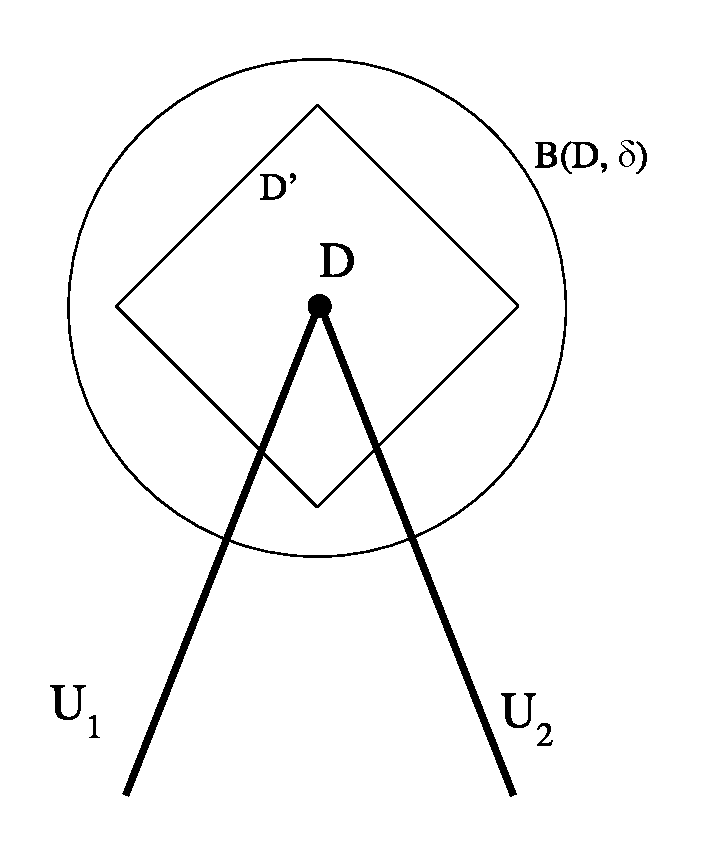
\includegraphics[width=0.24\textwidth]{figs/separated-proof-2} \hfill
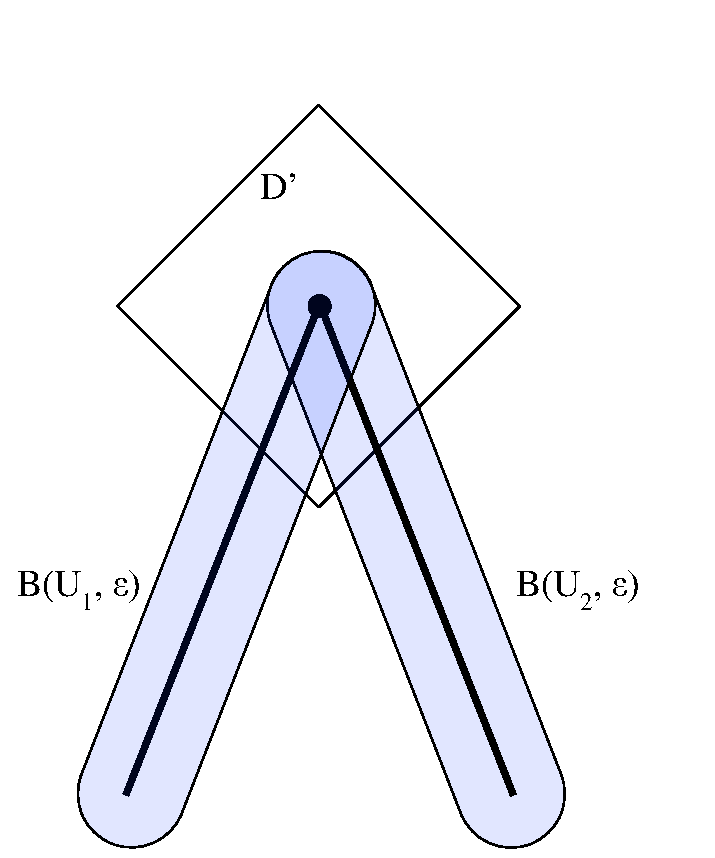
\includegraphics[width=0.24\textwidth]{figs/separated-proof-3} \hfill
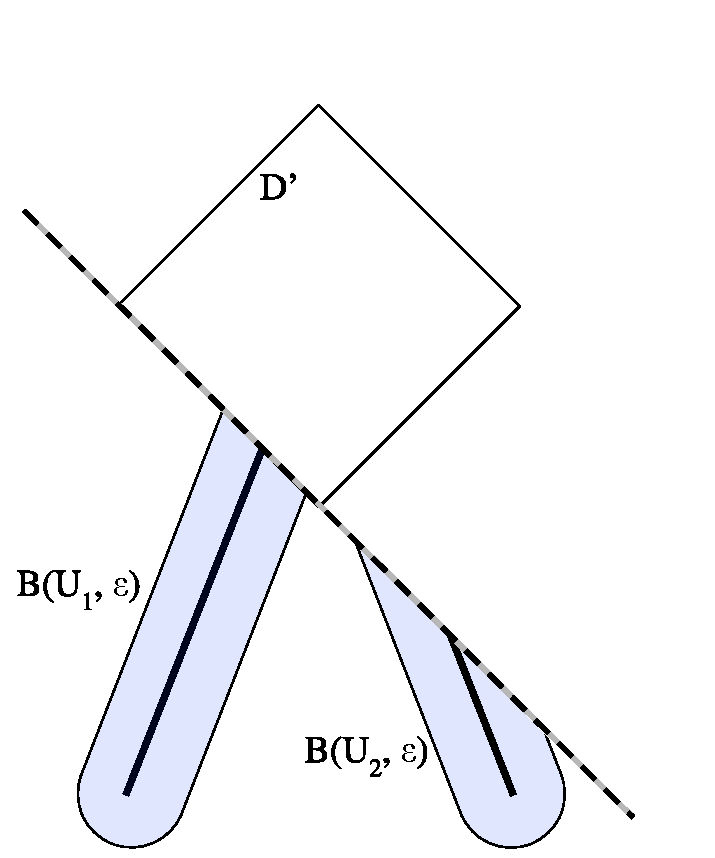
\includegraphics[width=0.24\textwidth]{figs/separated-proof-4} \hfill
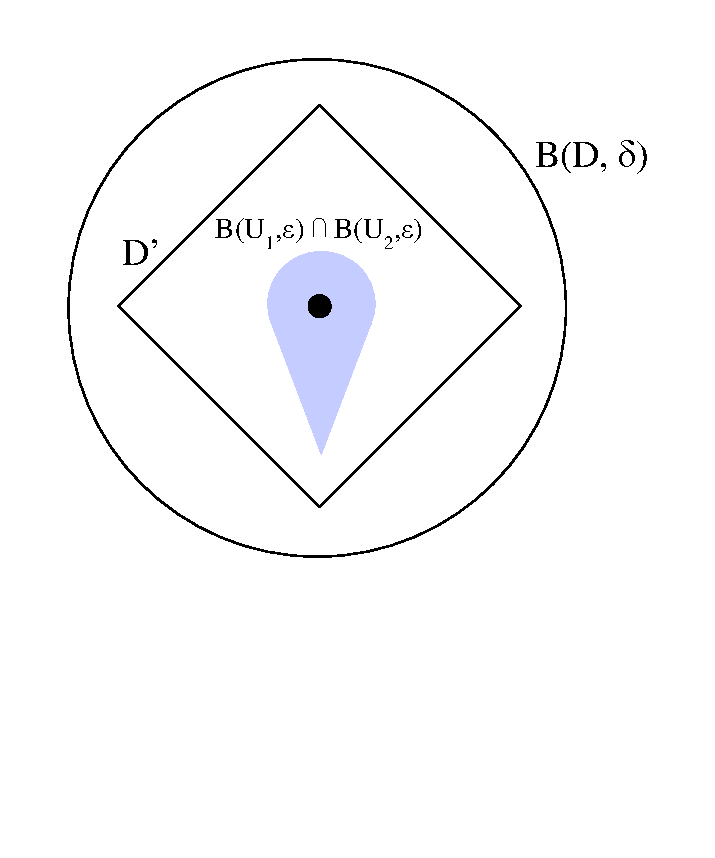
\includegraphics[width=0.24\textwidth]{figs/separated-proof-5}
\end{figure}

\begin{lemma} \label{lemma:thick-empty}
  Let $\{U_j : j \in \mathcal{J}\}$ be a finite collection of nonempty closed, convex sets with $\cap_{j\in\mathcal{J}} U_j = \emptyset$.
  Then for all $\delta > 0$, there exists  $\epsilon > 0$ such that $\cap_{j\in\mathcal{J}} B(U_j,\epsilon) = \emptyset$.
\end{lemma}
\begin{proof}
  By induction on the size of the family.
  Note that the family must have size at least two.
  Let $U_j$ be any set in the family and let $U' = \cap_{j' \neq j} U_{j'}$.
  There are two possibilities.

  The first possibility, which includes the base case where the size of the family is two, is the case $U'$ is nonempty.
  Because $U_j$ and $U'$ are non-intersecting closed convex sets, they are separated by some distance $\epsilon$.
  By Lemma \ref{lemma:thick-nonempty}, for any $\epsilon > 0$, there exists $\delta > 0$ such that $\cap_{j'\neq j} B(U_{j'},\delta) \subseteq B(U', \epsilon/3)$.
  Then we have $B(U_j, \epsilon/3) \cap B(U', \epsilon/3) = \emptyset$.

  The second possibility is that $U'$ is empty.
  This implies we are not in the base case, as the family must have three or more sets.
  By inductive assumption, for small enough $\delta$ we have $\cap_{j' \neq j} B(U_{j'},\delta) = \emptyset$, which proves this case.
\end{proof}


\begin{corollary} \label{cor:thick-intersect}
  There exists a small enough $\epsilon > 0$ such that, for any subset $\{U_j : j \in \mathcal{J}\}$ of $\U$, if $\cap_j U_j = \emptyset$, then $\cap_j B(U_j,\epsilon) = \emptyset$.
\end{corollary}
\begin{proof}
  For each subset, Lemma \ref{lemma:thick-empty} gives an $\epsilon$.
  We take the minimum over these finitely many choices.
\end{proof}

\begin{theorem} \label{thm:small-eps-thick}
  For all small enough $\epsilon$, the epsilon-thickened link $\psi$ (Definition \ref{def:eps-thick-link}) is a well-defined link function from $\R'$ to $\R$, i.e. $\psi(u) \neq \bot$ for all $u$.
\end{theorem}
\begin{proof}
  Fix a small enough $\epsilon$ as promised by Corollary \ref{cor:thick-intersect}.
  Consider any $u \in \R'$.
  If $u$ is not in $B(U,\epsilon)$ for any $U \in \U$, then we have $\Psi(u) = \R$, so it is nonempty.
  Otherwise, let $\{U_j : j \in \mathcal{J}\}$ be the family whose thickenings intersect at $u$.
  By Corollary \ref{cor:thick-intersect}, because of our choice of $\epsilon$, the family themselves has nonempty intersection.
  By Lemma \ref{lemma:calibrated-pos}, their corresponding report sets $\{R_j : j \in \mathcal{J}\}$ also intersect at some $r$, so $\Psi(u)$ is nonempty.
\end{proof}

In the rest of the section, for shorthand, we write $L(u;p) := \langle p, L(u) \rangle$ and similarly $\ell(r;p)$.

\begin{lemma} \label{lemma:exposed-shortest}
  Let $U$ be a convex, closed set and $u \not\in U$.
  Then $\inf_{u^* \in U} \|u-u^*\|$ is achieved by some unique $u^* \in U$.
  Furthermore, $u^*$ is the unique member of $U$ such that $u = u^* + \alpha v$ for some $\alpha > 0$ and unit vector $v$ that exposes $u^*$.
\end{lemma}
\begin{proof}
  Unique achievement of the infimum is well-known.
  (Achievement follows e.g. because the set $U \cap \{u' : \|u - u'\| \leq d(U,u) + 1\}$ is closed and compact, so the continuous function $u' \mapsto \|u-u'\|$ achieves its infimum.
  Uniqueness follows because for two different points $u',u''$ at the same distance from $u$, the point $0.5u' + 0.5u''$ is strictly closer and also lies in the convex set $U$.)
  Now suppose $u = u' + \alpha' v'$ where $v'$ is a unit vector exposing $u'$.
  Then $U$ is contained in the halfspace $\{u'': \langle u'', v'' \rangle \leq \langle u',v' \rangle \}$.
  But every point in this halfspace is distance at least $\alpha'$ from $u$, as $\|u-u''\| \geq \langle v, u - u'' \rangle \geq \langle v, u-u'\rangle = \alpha'$.
  So $u'$ uniquely achieves this minimum distance.
\end{proof}

\begin{lemma} \label{lemma:distance-loss}
  \raft{What I changed: linear ftn $\to$ affine; name the cell $U_f$ for $f$; also name set of functions $\F$, normals $V_f$, etc}
  If $L$ is a polyhedral loss, then for each $p$, there exists a constant $c$ such that, for all $u$,
    \[ L(u;p) - \inf_{u^* \in \R'} L(u^*;p) \geq c \cdot d(\Gamma(p),u) . \]
\end{lemma}
\begin{proof}
  Fix $p$ and let $U = \Gamma(p)$.
  If $u \in U$, then both sides are zero.
  So it remains to find a $c$ such that the inequality holds for all $u \not\in U$.

  $L(\cdot;p)$ is a convex polyhedral function, so it is the pointwise maximum over finitely many affine functions.
  Recall that $\risk{L}(p) = \min_{u} L(u;p)$, the Bayes risk.
  Construct the convex polyhedral function $\hat{L}(\cdot;p)$ by dropping from the maximum those affine functions that are never equal to $L$ for any $u^* \in U$.
  We have $\hat{L}(u^*;p) = \risk{L}(p)$ for all $u^* \in U$ and $\hat{L}(u;p) \leq L(u;p)$ for all $u \not\in U$.
  Now $\hat{L}$ is also a maximum over finitely many affine functions $\F$.
  Each such function $f\in\F$ is equal to $\hat{L}$ above a closed, convex cell $U_f\subseteq\reals^d$ in the power diagram formed by projecting $\hat{L}(\cdot;p)$.
  If $f$ has nonzero gradient, then $U_f \cap U$ is a face of $U$.
  We will prove that there exists $c_f > 0$ such that, for all $u\in U_f$,
    \[ \hat{L}(u;p) \geq \risk{L}(p) + c_f \cdot d(U,u) . \]
  Taking $c$ to be the minimum of $c_f$ over the finitely many $f\in\F$ with nonzero gradient (which covers all points $u \not\in U$) will complete the proof.

  Consider the set of unit vectors $V = \{v \in \reals^d : \|v\|=1\}$ and the boundary of $U$, denoted $\partial U$.
  For any $u^*\in\partial U$, $v\in V$ such that $v$ exposes $u^*$, let
  \raft{NOTE: we need to define ``exposes'' or just phrase in terms of normals: $v$ is normal to $U$ at $u^*$}
  $G_{u^*,v} = \left\{ u^* + \beta v : \beta \geq 0 \right\}$
  be the ray leaving $U$ from $u^*$ in direction $v$.
  % Note that $\{ u : u \not\in U\} \subseteq \cup_{u^*,v} G_{u^*,v}$.
  For each $f\in\F$, we define the set $R_f \subseteq \partial U \times V$ to be the points $(u^*,v)$ such that there exists $\epsilon>0$ with $G_{u^*,v} \cap U_f = G_{u^*,v} \cap B(u^*,\epsilon)$; that is, such that the ray $G_{u^*,v}$ starts its journey in $U_f$.
  Futhermore, define $U^*_{f,v} = \{u^* \in \partial U : (u^*,v)\in R_f\}$ and $V_f = \{v\in V: \exists u^*\in U_f\cap U,\: (u^*,v) \in R_f\}$.
  (That is, $U^*_{f,v}$ is the set of points from which the ray in direction $v$ begins in $U_f$, and $V_f$ is the set of all normal directions in which some ray begins in $U_f$.)
  Finally, define $G_f = \cup_{(u^*,v)\in R_f} G_{u^*,v}$ as the union of all such rays beginning in $U_f$.
  Note that $\cup_{f\in\F} G_f \supseteq \reals^d \setminus U$; this follows as every point not in $U$ is on a normal ray out of $U$, which must begin in some cell $U_f$.

  We will prove the following steps:
  \begin{enumerate}
  % \item For all $u^*\in\partial U$, $v\in V$ such that $v$ exposes $u^*$, there is some $f\in\F$ such that $u^* \in U_f$ and $G_{u^*,v} \cap U_f \neq \{u^*\}$.
  %   (That is, the ray $G_{u^*,v}$ begins its journey away from $U$ within $U_f$.)
    \item For all $f\in\F$, $v\in V_f$, there exists a constant $c_{f,v} > 0$ such that $L(u;p) \geq \risk{L}(p) + c_{f,v} \cdot d(U,u)$ for all $u \in G_{u^*,v}$ and all $u^*\in U^*_{f,v}$.
    \item For all $f\in \F$, the set $V_f$ is compact, and the map $v \mapsto c_{f,v}$ is continuous on $V_f$.
    \item Hence, there is an infimum $c_f > 0$ such that $f(u) \geq \risk{L}(p) + c_f \cdot d(U,u)$ for all $u\in G_f$.
    \item Let $c = \min \{c_f : f\in\F, \nabla f \neq 0\}$; then $L(u;p) \geq \risk{L}(p) + c \cdot d(U,u)$ for all $u \not\in U$.
  \end{enumerate}

  % (1) Follows because $G_{u^*,v}$ is contained in a cell of the power diagram, which is a set of points where $\hat{L}(\cdot;p) = f(\cdot)$. \bo{Should have more justification.}

  (1) Let $\nabla f$ denote the gradient of the affine function $f$.
  Note that because $u^*$ is on the boundary of $U$, we have $f(u^*) = \hat{L}(u^*;p) = \risk{L}(p)$.
  So we can write, using Lemma \ref{lemma:exposed-shortest},
  \begin{align*}
    f(u) &= f(u^*) + (\nabla f)\cdot (u - u^*)  \\
    f(u) &= f(u^*) + (\nabla f)\cdot (d(u^*,u) v)  \\
         &= \risk{L}(p) + c_{f,v} \cdot d(U,u)  \\
  \end{align*}
  where $c_{f,v} = (\nabla f)\cdot v$.
  We must have $c_{f,v} > 0$ because the set $U$ minimizes $L(\cdot;p)$, so $f(u) > f(u^*) = \risk{L}(p)$.
  The result now follows as $L(u;p) \geq \hat L(u;p) \geq f(u)$.

  (2) The intersection $U_f \cap U$ is a face of $U$, and thus decomposes as the union of relative interiors of subfaces, $U_f \cap U = \cup_i \mathrm{ri}(F_i)$.
  For each $i$, let $V_i = \{v\in V: \exists u^*\in \mathrm{ri}(F_i),\: (u^*,v)\in R_f\}$.
  % set $N_U(u^*)$ is the same for all $u^*\in\mathrm{ri}(F_i)$~\cite{lu2008normal}.
  % \raft{That is a total punt reference---not sure the result is in there, but it easily could be!}
  For any $v\in V_i$, we may consider the power diagram restricted to $A$, the affine hull of $\{u + \alpha v: u\in U, \alpha\in\reals\}$.
  As there is some $u^*\in U$ such that $(u^*,v)\in R_f$, in particular, $U_f\cap A$ intersects $A\cap\mathrm{ri}(F_i)$ and thus must contain $A\cap\mathrm{ri}(F_i)$.
  We conclude that $(u',v)\in R_f$ for all other $u'\in \mathrm{ri}(F_i)$.
  \raft{The idea here is that if you can start in $\mathrm{ri}(F_i)$ and move in direction $v$ and land immediately in $U_f$, then you can do that anywhere from $\mathrm{ri}(F_i)$; otherwise $U_f$ intersects only part of $\mathrm{ri}(F_i)$ (at least when restricting to $A$), a contradiction.}
  Thus, we have $\{(u^*,v) \in R_f : u^*\in F_i\} = F_i \times V_i$.
  For closure, pick any $u^*\in \mathrm{ri}(F_i)$, and consider a sequence $\{v_j\}_j$ with $(u^*,v_j)\in R_f$, and corresponding witnesses $\{\epsilon_j\}_j$.
  Then we have $u^* + \epsilon_j v_j \in U_f$ for all $j$, and as $u^*\in U_f$ and $U_f$ is closed and convex, the limiting point must be contained in $U_f$ as well.
  \raft{Thus is totally bogus actually, since the limiting point could be $u^*$ itself.  Need a different approach I think.}
  We have now shown $V_f$ to be the union of finitely many closed convex sets, and thus closed.
  Boundedness follows as $V$ is bounded.
  Finally, $c_{f,v}$ is linear in $v$, and thus continuous.

  Steps (3) and (4) are immediate and complete the proof.
\end{proof}

\begin{theorem} \label{thm:app-eps-thick-sep}
  For small enough $\epsilon$, the $\epsilon$-thickened link $\psi$ (Definition \ref{def:eps-thick-link}) satisfies that, for all $p$, there exists $\delta > 0$ such that, for all $u \in \R'$,
    \[ L(u;p) - \inf_{u^* \in \R'} L(u^*;p) \geq \delta \left[ \ell(\psi(u);p) - \min_{r^* \in \R} \ell(r^*;p) \right] . \]
\end{theorem}
\begin{proof}
  We take the $\epsilon$ thickened link, which is well-defined by Theorem \ref{thm:small-eps-thick}.
  Fix $p$ and let $U = \Gamma(p)$.
  The left-hand side is nonnegative, so it suffices to prove the result for all $u$ such that the right side is strictly positive, i.e. for all $u$ such that $\psi(u) \not\in \gamma(p)$.
  By definition of the $\epsilon$-thickened link, we must have $d(U,u) \geq \epsilon$.
  By Lemma \ref{lemma:distance-loss}, we have $L(u;p) - \inf_{u^*} L(u^*;p) \geq C$ where $C = c\epsilon$ for some $c > 0$.
  This holds for all $u$.
  Meanwhile,
    \[ \ell(\psi(u);p) - \min_{r^*} \ell(r^*;p) \leq \max_{r \in \R} \ell(r;p) - \min_{r^* \in \R} \ell(r^*;p) =: D, \]
  for some constant $D$.
  This also holds for all $u$.
  Set $\delta = \frac{C}{D}$ to complete the proof.
\end{proof}

\begin{proof}[Proof of Theorem \ref{thm:eps-thick-calibrated}]
  The two claims are Theorems \ref{thm:small-eps-thick} and \ref{thm:app-eps-thick-sep}.
\end{proof}

\section{Omitted Proofs}\label{app:omitted-proofs}
% While Definition~\ref{def:loss-embed} gives the notion of one \emph{loss} embedding another, we now generalize the notion of one \emph{property} embedding another. \jessie{Merge with earlier definitions if we keep this section}
% \begin{definition}\label{def:prop-embed}
%   A property $\Gamma : \simplex \toto \reals^d$ embeds a property $\gamma:\simplex \toto \R$ on a set $\Sc$ if there exists some injective embedding $\varphi:\R \to \reals^d$ such that for all $p \in \simplex$ and $r \in \R$, we have $r \in \gamma(p) \iff \varphi(r) \in \Gamma(p)$.
%   If there is a representative set $\Sc$ such that $\Gamma$ embeds $\gamma$ on $\Sc$, then we simply say $\Gamma$ embeds $\gamma$.
%   Moreover, we say a loss embeds a property when it embeds a loss eliciting the property.
% \end{definition}
% 
% 
% By condition (ii.) of Definition~\ref{def:loss-embed}, we then have $L$ embedding $\ell$ implies $\prop{L}$ embeds $\prop{\ell}$.
% However, Definitions~\ref{def:loss-embed} and~\ref{def:prop-embed} are not immediately equivalent because property embedding does not capture the requirement of matching losses on embedded points; i.e., that $L(\varphi(r)) = \ell(r)$ for all $r \in \R$.  
% However, Lemma~\ref{lem:embed-defs-equiv} shows an equivalence follows without loss of generality.
% 
% \begin{lemma}\label{lem:embed-defs-equiv}
%	% \raft{Introduce $L$}
%	Let $L : \reals^d \to \reals^\Y_+$ be a loss function whose infimum is attained in expectation for all $p \in \simplex$.
%	If the property $\Gamma := \prop{L}$ embeds the finite property $\gamma : \simplex \toto \R$, then there is a discrete loss $\ell:\R \to \reals^\Y_+$ such that $\ell$ elicits $\gamma$ and $L$ embeds $\ell$.
% \end{lemma}
% \begin{proof}
%   \raft{All the important pieces are here, but take it slower.  State $\ell$ as a definition (let $\ell$ be given by...) and show why $L$ embeds it.\jessie{Took another pass but changed technique, adding in this detail.  Now very similar to the proof of Prop 1 forward direction.}}
%   Consider the embedding $\varphi$ given by the property embedding and take the discrete loss $\ell:r \mapsto L(\varphi(r))$.
%   Now, we claim that $L$ embeds $\ell$, and by Proposition~\ref{prop:embed-bayes-risks}, we can simply show $\risk{L} = \risk{\ell}$, and the risks being polyhedral follows from $\ell$ being discrete.
%   
%   First, we show that for all $p \in \simplex$, we have $(1) \inf_{u \in \reals^d}\inprod{p}{L(u)} = (2) \inf_{r \in \R}\inprod{p}{L(\varphi(r))}$, and the equality of risks follows.
%   $(1) \leq (2)$ follows from the fact that $\varphi(\R) \subset \reals^d$ and definition of infimum. 
%   Consider that if we had $(1) < (2)$ for some $p \in \simplex$, then there would be no $r$ such that $\varphi(r) \in \Gamma(p)$, and therefore, we would have $\gamma(p) = \emptyset$, yielding a contradiction. 
%   This gives us $(1) = (2)$, so we have $\risk{L} = \risk{L|_{\varphi(\R)}} = \risk{\ell}$.
%	% 
%	% Now consider the property $\Gamma' := p \mapsto \Gamma(p) \cap \varphi(\R)$.
%	% We have $\Gamma'$ nondegenerate since $\Gamma$ embedding $\gamma$ implies that, for all $p \in \simplex$, there is some $r \in \R$ such that $\varphi(r) \in \Gamma(p)$.
%	% Therefore, for all $p \in \simplex$, we have $\inf_{r \in \R}\inprod{p}{L(\varphi(r))} = \inf_{r \in \R} \inprod{p}{\ell(r)}$, which yields $\risk{L|_{\varphi(\R)}} = \risk{\ell}$.
%	% Chaining the two equalities, we now have $\risk{L} = \risk{\ell}$.
%	
%	% To verify $\ell$ elicits $\gamma$, consider $r \in \gamma(p) \iff \varphi(r) \in \Gamma(p)$ by embedding, $ \iff \varphi(r) \in \argmin_{u \in \reals^d} \inprod{p}{L(u)}$ by $L$ eliciting $\Gamma$, and $ \iff r \in \argmin_{r \in \R} \inprod{p}{\ell(r)}$ by applying the definition of properties to the embedding definition.
%	% \hrule
%	%	If $\Gamma$ embeds a finite $\gamma$, $L$ must embed a discrete loss $\ell$ such that $\ell(r) = L(\varphi(r))$ for all $r \in \R$.  
%	%	Moreover, we can see $\ell$ elicits $\gamma$ since we have $r \in \gamma(p) \iff \varphi(r) \in \Gamma(p) \iff \varphi(r) \in \argmin_{u \in \reals^d} \inprod{p}{L(u)} \iff r \in \argmin_{r \in \R} \inprod{p}{\ell(r)}$.
%	% 
%	% \raft{Spell this out; I don't think these distributions are enough, for the same reason as above.  \jessie{Took a different approach of using Prop 1 to show the risks are equal.}}
%	%	The final condition of matching loss values is satisfied by considering the equality of the expected loss on each $\delta_y$ distribution.
% \end{proof}

\jessiet{GO THROUGH THIS}
When working with convex surrogates which are not strictly convex, one quickly encounters redundant properties: if $\inprod{p}{L(\cdot)}$ is minimized by a point where $\inprod{p}{L}$ is flat, then there will be an uncountable set of reports which also minimize the expected loss.
As results in property elicitation typically assume properties are non-redundant (e.g.~\cite{frongillo2014general,frongillo2015elicitation}), 
% it is useful to consider a transformation which removes redundant level sets, captured by the \emph{trim} operation.

\begin{definition}\label{def:trim}
  Given an elicitable property $\Gamma:\simplex \toto\R$, we define $\trim(\Gamma) = \{\Gamma_u : u \in \R \text{ s.t. } \neg\exists u'\in\R,u'\neq u,\, \Gamma_u \subsetneq \Gamma_{u'}\}$ as the set of maximal level sets of $\Gamma$.
\end{definition}
\jessie{Do we want to re-define $\trim(\Gamma) = \{\Gamma_r \mid r \in \Sc\}$ for any minimum representative set $\Sc$?}

% \btw{RF: Note for later: should be able to show that the union of trim is the simplex.\jessie{This is part of the proposition statement 2 now.}}
% Take note that the unlabeled property $\trim(\Gamma)$ is non-redundant, meaning that for any $\theta \in \trim(\Gamma)$, there is no level set $\theta' \in \trim(\Gamma)$ such that $\theta \subset \theta'$; this is a corollary of Proposition~\ref{prop:embed-trim}.


Before we state Proposition~\ref{prop:embed-trim}, we will need to general lemmas about properties and their losses.
The first follows from standard results relating finite properties to power diagrams (see Theorem~\ref{thm:aurenhammer}), and its proof is omitted.
The second is closely related to the definition of the trim operator: it states that if some subset of the reports are always represented among the minimizers of a loss, then one may remove all other reports and elicit the same property (with those other reports removed).

\begin{lemma}\label{lem:finite-full-dim}
  Let $\gamma$ be a finite (non-redundant) property elicited by a loss $L$.
  Then the negative Bayes risk $G$ of $L$ is polyhedral, and the level sets of $\gamma$ are the projections of the facets of the epigraph of $G$ onto $\simplex$, and thus form a power diagram.
  In particular, the level sets of $\gamma$ are full-dimensional in $\simplex$ (i.e.,\ of dimension $n-1$).
\end{lemma}

\btw{Commented out result about old trim def = new trim def - Jessie 2 June 21}
%\btw{JESSIE: Figures/an example might help clarify this}
%When a property $\Gamma$ embeds a finite property $\gamma$, we can show that the level sets of $\gamma$ correspond exactly to their embedded level sets of $\Gamma$, and that these embedded level sets are exactly $\trim(\Gamma)$.
%\jessiet{This lemma new to journal version}
%\begin{lemma}\label{lem:embedded-level-sets-trim}
%  Let $\Gamma$ be an elicitable property.
%  If $\Gamma$ embeds a (non-redundant) finite property $\gamma : \simplex \toto \R$ by the injection $\varphi$, then $\{\gamma_r : r \in \R\} = \{\Gamma_u : u \in \varphi(\R)\} = \trim(\Gamma)\proposedadd{=\trim(\gamma)}$.
%  \proposedadd{RETRY: Let $\Gamma$ be an elicitable property.
%    If $\Gamma$ embeds a finite property $\gamma : \simplex \toto \R$ by the injection $\varphi$, then for any minimum representative set $\Sc$ for $\gamma$, we have $\{\gamma_r : r \in \Sc\} = \{\Gamma_u : u \in \varphi(\Sc)\} = \trim(\Gamma)=\trim(\gamma)$.}
%\end{lemma}
%\begin{proof}
%  Let $L$ elicit $\Gamma$.
%  Take $\ell$ to be the loss embedded by $L$ from Lemma~\ref{lem:embed-defs-equiv}.
%  Moreover, by Proposition~\ref{prop:embed-bayes-risks}, we have $\risk{L} = \risk{\ell}$.
%  % \raft{Implicitly? Justify the claim.  \jessie{In definition of finite properties, we say that we assume we are talking about non-redundant.}}
%  As $\gamma$ is finite (and non-redundant by assumption), we know that each level set of $\gamma$ must be full-dimensional in $\affhull(\simplex)$. 
%  For all $r \in \R$, we know $\gamma_r = \Gamma_{\varphi(r)}$, so we must also have $\Gamma_{\varphi(r)}$ full-dimensional.
%  Moreover, we have $\{\gamma_r : r \in \R\} = \{\Gamma_{\varphi(r)} : r \in \R\}$ as a corollary since this is true for each $r \in \R$.
%  \raft{The main action is here.  (1) Epigraph of $-\risk{L}$. (2) There is really only one case: every level set is a face of the power diagram, which must be contained (weakly, so $\subseteq$) in a facet. (3) To show that level sets are faces, you'll want to appeal to some piece of a proof in the prev section.}
%  Since the cell $\Gamma_{\varphi(r)}$ is the projection of a facet of the epigraph of $-\risk{L}$, which is convex, any other level set intersecting $\Gamma_{\varphi(r)}$ can be considered as faces of the epigraph of $-\risk{L}$, and therefore a face of the induced power diagram.
%  Therefore, we remove lower-dimensional faces, as they are proper subsets of the level sets of embedded reports, and conclude such $\Gamma_u \not \in \trim(\Gamma)$.
%  % in one of two cases:
%  % First, if the level set $\Gamma_u$ (for $u \not \in \varphi(\R)$) is a projection of a lower-dimensional face of $\risk{L}$, which is contained in a facet of the epigraph.
%  % Therefore, we must have $\Gamma_u \subset \Gamma_{\varphi(r)}$ for some $r \in \R$, and therefore $\Gamma_u \not \in \trim(\Gamma)$.
%  
%  Second, $\Gamma_u = \Gamma_{\varphi(r)}$ for some $r \in \R$, then the level set is in both $\{\Gamma_{\varphi(r)} : r \in \R\}$ and $\trim(\Gamma)$.
%
%  \proposedadd{First, construct $\Sc := \Sc(L)$ as Definition~\ref{cons:rep-set}\jessiet{Argue there is a bijection from this set to any other minimum representative set}, which is a minimum representative set by Proposition~\ref{prop:SL-minimum}. 
%    Moreover, we have $r \in \gamma(p) \iff \varphi(r) \in \Gamma(p)$ by embedding, and therefore $\gamma_r = \Gamma_{\varphi(r)}$, yielding $\{\gamma_r \mid r \in \Sc\} = \{\Gamma_{\varphi(r)} \mid r \in \Sc\}$ as this is true for all $r \in \Sc$.}
%
%  \proposedadd{Now let $T := \{\gamma_r \mid r \in \Sc\} = \trim(\gamma)$. 
%    First, if $\gamma_r \in T$, then it is not a subset of any level set as $\gamma_r$ is full-dimensional in the simplex as it corresponds to a facet of the epigraph of the negative risk $E_\ell$, and the supporting hyperplane is therefore unique.
%    Now, if $\theta \in \trim(\gamma)$, then there is some report $r'$ such that $\theta = \gamma_{r'}$.
%    If $r' \not \in \Sc$, we want to claim there is some $r$ such that $\gamma_{r'} = \gamma_r$.
%    As $\theta$ is a maximal level set, it has a nonempty interior.
%    Therefore, for any $p \in \inter{\theta}$ (and one such $p$ must exist), the hyperplane $p \mapsto (p, \ell(r'))$ uniquely supports the epigraph of negative risk.
%    If $r' \not \in \Sc$, then there must be some $r \in \Sc$ such that $p \mapsto (p, \ell(r))$ also supports the same facet of $E_\ell$; if no such $r \in \Sc$ existed, we would contradict our claim that $\Sc$ is representative for $\ell$.
%    Similarly, we have $\{\Gamma_u \mid u \in \varphi(\Sc)\} = \trim(\Gamma)$ by the same logic.}
%\end{proof}

%\jessiet{03.01.21 - Old version of Prop~\ref{prop:embed-trim} moved to comment}
% \jessiet{Can we remove this?}
% \begin{proof}[Original]
%   Let $L$ elicit $\Gamma$.
%   
%   1 $\Rightarrow$ 2:
%   By the embedding condition, taking $\R_1 = \reals^d$ and $\R_2 = \varphi(\R)$ satisfies the conditions of Lemma~\ref{lem:loss-restrict}: for all $p\in\simplex$, as $\gamma(p) \neq \emptyset$ by definition, we have some $r\in\gamma(p)$ and thus some $\varphi(r) \in \Gamma(p)$.
%   Let $G(p) := -\min_{u\in\reals^d} \inprod{p}{L(u)}$ be the negative Bayes risk of $L$, which is convex, and $G_{\R}$ that of $L|_{\varphi(\R)}$.
%   By the Lemma, we also have $G = G_\R$.
%   As $\gamma$ is finite, $G$ is polyhedral.
%   Moreover, the projection of the epigraph of $G$ onto $\simplex$ forms a power diagram, with the facets projecting onto the level sets of $\gamma$, the cells of the power diagram.
%   (See Theorem~\ref{thm:aurenhammer}.)
%   As $L$ elicits $\Gamma$, for all $u\in\reals^d$, the hyperplane $p\mapsto \inprod{p}{L(u)}$ is a supporting hyperplane of the epigraph of $G$ at $(p,G(p))$ if and only if $u\in\Gamma(p)$.
%   This supporting hyperplane exposes some face $F$ of the epigraph of $G$, which must be contained in some facet $F'$.
%   Thus, the projection of $F$, which is $\Gamma_u$, must be contained in the projection of $F'$, which is a level set of $\gamma$.
%   We conclude that $\Gamma_u \subseteq \gamma_r$ for some $r\in\R$.
%   Hence, $\trim(\Gamma) = \{\gamma_r : r\in\R\}$, which is finite, and unions to $\simplex$.
%   
%   2 $\Rightarrow$ 3: let $\R = \{u_1,\ldots,u_k\} \subseteq\reals^d$ be a set of distinct reports such that $\trim(\Gamma) = \{\Gamma_{u_1},\ldots,\Gamma_{u_k}\}$.
%   Now as $\cup\,\trim(\Gamma) = \simplex$, for any $p\in\simplex$, we have $p\in\Gamma_{u_i}$ for some $u_i\in\R$, and thus $\Gamma(p) \cap \R \neq \emptyset$.
%   We now satisfy the conditions of Lemma~\ref{lem:loss-restrict} with $\R_1 = \reals^d$ and $\R_2 = \R$.
%   The property $\gamma:p\mapsto\Gamma(p)\cap\R$ is non-redundant by the definition of $\trim$, finite, and elicitable.
%   Now from Lemma~\ref{lem:finite-full-dim}, the level sets $\Theta = \{\gamma_r:r\in\R\}$ are full-dimensional, and union to $\simplex$.
%   Statement 3 then follows from the fact that $\gamma_r = \Gamma_r$ for all $r\in\R$.
%   
%   3 $\Rightarrow$ 1: let $\Theta = \{\theta_1,\ldots,\theta_k\}$.
%   For all $i\in\{1,\ldots,k\}$ let $u_i\in\reals^d$ such that $\Gamma_{u_i} = \theta_i$.
%   Now define $\gamma:\simplex\toto\{1,\ldots,k\}$ by $\gamma(p) = \{i : p\in\theta_i\}$, which is non-degenerate as $\cup\,\Theta = \simplex$.
%   By construction, we have $\gamma_i = \theta_i = \Gamma_{u_i}$ for all $i$, so letting $\varphi(i) = u_i$ we satisfy the definition of embedding, namely statement 1.
% \end{proof}






% \begin{lemma}\label{lem:fdls-in-trim}
%   If $\theta$ is a full-dimensional level set (in the simplex) of the elicitable property $\Gamma$, then $\theta \in \trim(\Gamma)$.
% \end{lemma}
% \begin{proof}
%   Let $u$ be the report such that $\theta = \Gamma_u$.
%   If there is a $u'$ so that $\Gamma_u = \Gamma_{u'}$, one of the level sets is in $\trim(\Gamma)$, and then we have $\theta$ equal to that level set.
%   If $\Gamma_u \subsetneq \Gamma_{u'}$, then either $\Gamma_u$ is not a full-dimensional level set or $\Gamma_u \cap \Gamma_{u'}$ is full-dimensonal.
%   If $\Gamma_u$ is not full-dimensional, then we contradict our assumption.
%   If $\Gamma_u \cap \Gamma_{u'}$ is full dimensional, then we contradict our elicitability condition (Lemma~\ref{lem:elicitable-level-sets}).
%   Therefore, full-dimensional level sets of an elicitable property must be in the trim operation of the same property.
% \end{proof}



\section{Lov\'asz Hinge}\label{app:lovasz}

The Lov\'asz hinge, introduced by~\citet{yu2018lovasz}, is a (convex) polyhedral surrogate for discrete losses described in terms of a submodular function, based on the well-known Lov\'asz extension.
We will study this surrogate using our framework, first identifying the loss it embeds, and then leveraging this loss to find a proof of inconsistency.
As defining the Lov\'asz hinge takes care, we begin with definitions.

\subsection{Notation and Definitions}
Let $N = \{1,\ldots,k\}$ be the index set for our binary predictions, with outcomes $\Y = 2^N$ corresponding to the set of labels which are assigned $+1$.
To map to the usual labels $\{-1,1\}$, for any $S\subseteq N$, we let $\ones_S \in \{0,1\}^k$ with $(\ones_S)_i = 1 \iff i\in S$ be the 0-1 indicator for $S$, and we let $\chi_S \in \{-1,1\}^k$ with $\chi_S = 2\ones_S - \ones$ be the $\pm 1$ indicator.
For clarity of exposition, we will depart from our usual notation for loss functions, writing a discrete loss $\ell : \R \times \Y \to \reals$ and surrogate $L : \reals^k \times \Y \to \reals$, and writing expected loss $L(u;p)$.
The link will be the sign function $\psi = \sgn$, with ties broken arbitrarily.

A set function $f:2^N\to\reals$ is \emph{submodular} if for all $S,T\subseteq N$ we have $f(S) + f(T) \geq f(S\cup T) + f(S\cap T)$.
A function is \emph{supermodular} if the inequality is reversed, and \emph{modular} if it holds with equality, for all $S,T\subseteq N$.
The function $f$ is \emph{increasing} if we have $f(S\cup T) \geq f(S)$, again for all $S,T\subseteq N$.

We are interested in convex surrogates for the following discrete loss $\ell:\R\times\Y\to\reals$, where $\R=\Y=2^N$,
\begin{equation}
\label{eq:discrete-set-loss}
\ell^f(A,S) = f(A\triangle S)~,
\end{equation}
where $\triangle$ is the symmetric difference operator, defined by $S\triangle T = (S\setminus T) \cup (T\setminus S)$.
Note: throughout we assume $\triangle$ has operator precedence over $\setminus$, $\cap$, and $\cup$.
In words, $\ell^f$ measures the joint error of our $k$ predictions by computing the set of mispredictions (elements in $A$ but not $S$ and vice versa) and calling the set function $f$.

A natural approach to deriving convex surrogates in the case of submodular functions $f$ is the Lov\'asz extension, which is known to be convex when $f$ if (and only if) submodular. %\jessiet{Doesn't make grammatical sense to me.}
Given any set-valued function $f:2^N\to\reals$, its \emph{Lov\'asz extension} $F:\reals^k\to\reals$ is given by
\begin{equation}\label{eq:lovasz-ext}
F(u) = \E[f(\{i:u_i \geq \Theta\})]~,
% F(u) = \sum_{i=1}^k u_{j_i} (f(\{j_1,\ldots,j_i\}) - f(\{j_1,\ldots,j_{i-1}\})~,
\end{equation}
where $\Theta$ is a uniformly distributed random variable on $[0,1]$.
There are several equivalent formulations for the Lov\'asz extension; see~\citet[Definition 3.1]{bach2013learning}.

Given set function $f$ with Lov\'asz extension $F$, \citet{yu2018lovasz} define the \emph{Lov\'asz hinge} as the loss $L^f:\reals^k\times\Y\to\reals$ given by
\begin{equation}
\label{eq:lovasz-hinge}
L^f(u,S) =
\begin{cases}
F\bigl((\ones - u \odot \chi_S)_+\bigr) & \text{if $f$ is increasing}
\\
\bigl(F(\ones - u \odot \chi_S)\bigr)_+ & \text{otherwise}
\end{cases}~,
\end{equation}
where $v (u \odot y)_i = u_iy_i$ is the Hadamard (element-wise) product and $((u)_+)_i = \max(u_i,0)$.
In what follows, we focus on the increasing case, which is the most natural: when you make an additional error, your loss cannot decrease.

\subsection{What does $L$ embed?}

From well-known facts about the Lov\'asz extension (see Lemma~\ref{lem:lovasz-trim} below), $L^f$ is certainly polyhedral, and thus by our framework we know it must embed a discrete loss $\hat\ell^f$, which may or may not be the same as $\ell^f$.
As with the top-$k$ example, we begin our analysis by calculating $\hat\ell^f$.

Let $\Gamma^f = \prop{L^f}$ and $\U = \{-1,0,1\}^k$.
Note that, for disjoint sets $A,B \subseteq N$, we have $\chi_A + \ones_B \in \U$, which at coordinate $i$ evaluates to $1$ for $i\in A$, $0$ for $i\in B$, and $-1$ otherwise.
Moreover, every point in $\U$ can be uniquely described in this way.
Finally, observe $\chi_A + \ones_B = \chi_A \odot \ones_{N\setminus B}$.

We will show that for every distribution $p$, an element of $\U$ is always represented in the minimizers of $L^f$, i.e., $\Gamma^f(p)$.
First, we show that we may restrict to the filled hypercube $[-1,1]^k$ without loss of generality.

\begin{lemma}
	\label{lem:lovasz-cube}
	Let $f:2^N\to\reals_+$ be increasing and normalized.
	Then for all $p\in\simplex$, $\Gamma(p) \cap [-1,1]^k \neq \emptyset$.
\end{lemma}
\begin{proof}
	Let $u\in\Gamma^f(p)$ such that $|u_i|>1$ for some $i\in [k]$, and furthermore suppose $|u_i|$ is the smallest value among all such coordinates, i.e., $|u_i| = \min\{|u_j| : |u_j| > 1\}$.
	We show that $u'\in\Gamma^f(p)$ where $u'_j = u_j$ for $j\neq i$ and $u'_i = \sgn(u_i)$ so that $|u'_i|=1$; the result then follows by iterating this argument until there are no entries with $|u_i|>1$.
	In fact, we will show the stronger statement that for all $S\in\Y$, $L^f(u',S) \leq L^f(u,S)$.
	Let $w = \ones - u\odot \chi_S$ and $w' = \ones - u'\odot \chi_S$, and note that $L^f(u,S) = F(w_+)$ and $L^f(u',S) = F(w'_+)$.
	
	First, consider the case that $(\chi_S)_iu_i > 0$; that is, if $u_i > 0$ and $i\in S$, or $u_i < 0$ and $i\notin S$.
	Here $1-(\chi_S)_iu_i = 1-|u_i| < 0$, so $w_i < 0$.
	For $u'$, we similarly have $w'_i = 1-|u'_i| = 0$.
	As $u$ and $u'$ differ only at index $i$, the same holds for $w$ and $w'$; we thus have $w_+ = w'_+$, so the loss remains unchanged.
	
	In the other case, $(\chi_S)_iu_i < 0$, we have $w_i = 1+|u_i| > 2$ and $w'_i = 1+|u'_i| = 2$, and again the other entries are identical.
	In particular, $w'_i \leq w_i$.
	Moreover, we claim that there is no other value in between, i.e.,\ there is no index $j\neq i$ such that $w'_i < w_j < w_i$.
	This follows from our assumption on $i$: if we had such a $j$, then we must have $2 < 1 - (\chi_S)_ju_j < 1 + |u_i|$, which can only occur when $\sgn(u_j) \neq \chi_S$, and thus $-(\chi_S)_ju_j = |u_j|$; we conclude $1 < |u_j| < |u_i|$, a contradiction.
	Thus, for all $j\neq i$, we have either $w_j \leq w'_i \leq w_i$ or $w'_i \leq w_i \leq w_j$.
	In light of $w'_j = w_j$, this is equivalent to either (a) $w_j \leq w_i$ and $w'_j \leq w'_i$, or (b) $w_i \leq w_j$ and $w'_i \leq w'_j$.
	Thus, there is a permutation $\pi$ which orders the elements of both $w$ and $w'$ simultaneously: for all $j,j'\in [k]$, $j<j'$, we have both $w_{\pi_j} \geq w_{\pi_{j'}}$ and $w'_{\pi_j} \geq w'_{\pi_{j'}}$.
	By another common representation of the Lov\'asz extension~\cite[Equation 3.1]{bach2013learning}, we thus have $F(w_+) - F(w'_+) = ((w_+)_i - (w'_+)_i)(f(T\cup\{i\})-f(T)) = (|u_i|-1)(f(T\cup\{i\})-f(T)) > 0$,
	where $T = \{\pi_1,\ldots,\pi_j\}$ such that $\pi_{j+1} = i$, and we have used the fact that $f$ is increasing and $|u_i|>1$.
	%\jessiet{I think this should technically be a $\geq 0$, since we have no notion of ``strictly increasing'' so even if $f$ is increasing, we could still have $f(T\cup\{i\})-f(T) = 0$.  Doesn't affect the result though.}
\end{proof}

From Lemma~\ref{lem:lovasz-cube}, we may now simplify the loss.
When $u\in[-1,1]^k$, we simply have $L^f(u,S) = F(\ones - u \odot \chi_S)$, as the coordinates of the input to $F$ are nonnegative.
We now further restrict to $\U$.

\begin{lemma}
	\label{lem:lovasz-trim}
	Let $\Gamma = \prop{L^f}$.
	Then for all $p\in\simplex$, $\Gamma(p) \cap \U \neq \emptyset$.
\end{lemma}
\begin{proof}
	We will construct polytopes $P^A_\pi \subseteq [-1,1]^k$ for every set $A\subseteq N$ and permutation $\pi \in N^N$, satisfying three conditions: (i) these polytopes cover the hypercube, meaning $\cup_{A,\pi} P^A_\pi = [-1,1]^k$, (ii) $P^A_\pi$ is the convex hull of points in $\U$, and (iii) for all $S\subseteq N$, $L(\cdot,S)$ is linear on $P^A_\pi$.
	The result will then follow, as $L(\cdot;p)$ will be also linear on each $P^A_\pi$, and thus minimized at a vertex.
	
	To begin, let us recall the polyhedra on which the Lov\'asz extension is linear; for any permutation $\pi$, define $P_\pi = \{u\in\reals^k : u_{\pi_1} \geq \cdots \geq u_{\pi_k}\}$.
	It is clear from the definition that $F$ is linear on $P_\pi$; see also Equation 3.1, and ``Linear interpolation on simplices'' (pg.\ 167) in \citet{bach2013learning}.
	We will use these polyhedra to identify the regions where $L(\cdot,S)$ is linear simultaneously for all outcomes $S\in\Y$.
	For any $A\subseteq N$ and permutation $\pi$, let
	\begin{equation}
	\label{eq:poly-pi}
	P^A_\pi = \{u\in[-1,1]^k : u \odot \chi_A \in P_\pi \cap \reals^k_+\}~.
	\end{equation}
	That is, $P^A_\pi$ contains all points $u$ such that $u \odot \chi_A$ is nonnegative (meaning $\sgn(u)$ matches $\chi_A$, breaking ties at $0$ favorably) and such that the coordinates of $u \odot \chi_A$ are in increasing order according to $\pi$.
	
	Condition (i) follows immediately: for any $u\in[-1,1]^k$, let $A = \{i:u_i\geq 0\}$, and $\pi$ be any permutation ordering the elements of $u \odot \chi_A$.
	For condition (ii), note that for any $u\in P^A_\pi$, as $u\odot \chi_A \in P_\pi$ we may write
	\begin{equation}
	\label{eq:udot-conv}
	u \odot \chi_A = \sum_{i=1}^{k-1} \left[ \left( u_{\pi_i} (\chi_A)_{\pi_i} - u_{\pi_{i+1}} (\chi_A)_{\pi_{i+1}} \right) \ones_{\{\pi_1,\ldots,\pi_i\}} \right] + u_{\pi_k} (\chi_A)_{\pi_k} \ones
	% + (1-u_{\pi_1}(\chi_A)_{\pi_1} \cdot 0
	~,
	\end{equation}
	%\jessiet{The indicator notation is confusing to me with the ones vector also in the same context.  That's just a personal opinion though.}
	%\jessiet{Unclear to me at first what the summation is over.  Added brackets to clarify.}
	which is a convex combination (again, see \citet[pg.\ 167]{bach2013learning}).
	We simply apply the involution $\odot\chi_A$ again, to obtain
	\begin{equation}
	\label{eq:udot-conv}
	u = \sum_{i=1}^{k-1} \left( u_{\pi_i} (\chi_A)_{\pi_i} - u_{\pi_{i+1}} (\chi_A)_{\pi_{i+1}} \right) \ones_{\{\pi_1,\ldots,\pi_i\}}\odot \chi_A + u_{\pi_k} (\chi_A)_{\pi_k} \chi_A
	% + (1-u_{\pi_1}(\chi_A)_{\pi_1} \cdot 0
	~,
	\end{equation}
	and condition (ii) follows as $\ones_B \cdot \chi_A \in \U$ for all sets $B\subseteq N$.
	%\jessiet{What is $B$ here? I might just be slow, but I missed the step where this leads to Condition (ii)}
	
	Finally, for condition (iii), fix a subset $A\subseteq N$ and permutation $\pi$.
	For each outcome $S\subseteq N$, we will construct an alternate permutation $\pi^S$ such that for all $u\in P^A_\pi$ we have $\ones - u\odot\chi_S \in P_{\pi^S}$.
	As $F$ is linear on $P_{\pi'}$ for all permutations $\pi'$, we will conclude that for any fixed subset $S$ the loss $L(u,S) = F(\ones - u\odot\chi_S)$ will be linear in $u$ on $P^A_\pi$.
	
	To construct $\pi^S$, we ``shatter'' the permutation $\pi$ into two pieces, depending on whether an index is in $A\triangle S$ or not.
	In particular, note that if $i\in A\triangle S$, then for all $u\in P^A_\pi$ we have $u_i(\chi_A)_i \geq 0$ and $(\chi_A)_i = -(\chi_S)_i$, so $(\ones - u\odot\chi_S)_i = 1 - u_i(\chi_S)_i = 1 + u_i(\chi_A)_i \geq 1$.
	Similarly, when $i\notin A\triangle S$, then $(\chi_A)_i = (\chi_S)_i$, so $(\ones - u\odot\chi_S)_i = 1 - u_i(\chi_S)_i = 1 - u_i(\chi_A)_i \leq 1$.
	As $\pi$ orders the elements $u_i(\chi_S)_i$ in decreasing order, we see that the following permutation $\pi^S$ will order the elements of $\ones - u\odot\chi_S$ in decreasing order: sort the elements in $A\triangle S$ according to $\pi$, followed by the remaining elements according to the reverse of $\pi$.
	As the definition of $\pi^S$ is independent of $u$, we see that $u\in P^A_\pi \implies \ones - u\odot\chi_S \in P_{\pi^S}$, as desired.
\end{proof}

We can now see that $L^f$ embeds the loss given by $L^f$ restricted to $\U$, as $\U$ is a finite set.
In fact, we can write this loss entirely in terms of $f$ itself.

\begin{lemma}
	\label{lem:lovasz-u}
	Let $\hat\ell^f:\hat\R\times\Y\to\reals_+$, where $\hat\R = \{(A,B) \in 2^N \times 2^N: A\cap B=\emptyset\}$, be given by
	\begin{equation}
	\label{eq:lovasz-embeds}
	\hat\ell^f((A,B),S) = L^f(\chi_A + \ones_B,S) = f(A\triangle S\setminus B) + f(A\triangle S\cup B)~.
	\end{equation}
	Then the Lov\'asz hinge $L^f$ embeds $\hat\ell^f$.
\end{lemma}
\begin{proof}
	As observed above, the set $\U$ is in bijection with $\hat \R$, using the transformation $u = \chi_A + \ones_B$.
	As also observed above, we may write $u = \chi_A \odot \ones_{N\setminus B}$ as well.
	Combining Lemma~\ref{lem:lovasz-trim} with \ref{lem:loss-restrict}, we see that $L^f$ embeds $L^f|_\U$.
	It thus only remains to verify the form~\eqref{eq:lovasz-embeds}.
	We have $L^f(u,S) = F(x)$ where $x = \ones - u\odot\chi_S = \ones - \ones_{N\setminus B} \odot \chi_A \odot \chi_S = \ones + \ones_{N\setminus B} \odot \chi_{A\triangle S} = \ones_{B} + 2\ones_{A\triangle S\setminus B}$.
	%\jessiet{This next line lost me.}
	As $(A\triangle S \setminus B) \cup B = A\triangle S \cup B$, the result follows from~\cite[Prop 3.1(h)]{bach2013learning}.
\end{proof}

From the form~\eqref{eq:lovasz-embeds}, we see that $\hat\ell^f$ matches $2\ell$ when $B=\emptyset$, just as hinge loss embeds twice 0-1 loss.
When $B$ is nonempty, it acts as an ``abstain set'', guaranteeing some loss in the second term, but removing errors in the first term.

\subsection{Inconsistency}

In light of the previous results, we can see that to show inconsistency we may focus on reports $(A,B)$ with $B\neq\emptyset$.
Intuitively, if such a report is ever optimal, then $L^f$ has a ``blind spot'' with respect to the indices in $B$, and we can leverage this to ``fool'' $L^f$.
In particular, we will focus on the uniform distribution $\bar p$ on $\Y$, and perturb it slightly depending on $B$ to find an optimal point $u\in\U$ which maps to a suboptimal report.
In fact, we will show that one can always find such a point violating calibration, unless $f$ is modular.

Given our focus on the uniform distribution, the following definition will be useful: for any set function $f$, let $\bar f := \E_{S\sim \bar p}[f(S)] = 2^{-k} \sum_{S\subseteq N} f(S)$.
The next two lemmas relate $\bar f$ and $f(N)$ to expected loss and modularity.

\begin{lemma}
	\label{lem:2-bar-f}
	For all $(A,B) \in \hat\R$, $\hat\ell^f((A,B);\bar p) \geq f(N)$. %\jessiet{Intuitively, this seems backwards?  Since $f$ is increasing.  But that might be the point.}
	For all $A\subseteq N$, $\hat\ell^f((A,\emptyset);\bar p) = 2\bar f$.
\end{lemma}
\begin{proof}
	Letting $\overline B := N\setminus B$ for short %\jessiet{To make notation more consistent, maybe change $\overline B$ to $B^c$ so something else to deviate from the average notation.}, we have
	\begin{align*}
	\hat\ell^f((A,B);\bar p)
	&= 2^{-k} \sum_{S\subseteq N} f(A\triangle S\setminus B) + f(A\triangle S\cup B)
	\\
	&= 2^{-|\overline B|} \sum_{T\subseteq \overline B} f(T) + f(T\cup B)
	\\
	&= \frac 1 2 \; 2^{-|\overline B|} \sum_{T\subseteq \overline B} f(T) + f(\overline B\setminus T) + f(T\cup B) + f((\overline B\setminus T)\cup B)
	\\
	&\geq \frac 1 2 \left( f(\overline B) + f(\emptyset) + f(N) + f(B) \right)
	\\
	&\geq \frac 1 2 \left( f(N) + f(N) \right) = f(N)~,
	\end{align*}
	where we use submodularity in both inequalities.
	%\jessiet{I didn't see how we got from first line to second until this little reminder that $B = \emptyset$ below-- any chance we can move that above the arithmetic?}
	The second statement follows from the second equality above after setting $B=\emptyset$, as then $\overline B = N$ and thus $T$ ranges over all of $2^N$.
\end{proof}

\begin{lemma}
	\label{lem:bar-f}
	Let $f$ be submodular and normalized.
	Then $\bar f \geq f(N)/2$, and $f$ is modular if and only if $\bar f = f(N)/2$.
\end{lemma}
\begin{proof}
	The inequality follows from Lemma~\ref{lem:2-bar-f} with $B=\emptyset$.
	Next, note that if $f$ modular we trivially have $\bar f = f(N)/2$.
	If $f$ is submodular but not modular, we must have some $S\subseteq N$ and $i\in S$ such that $f(S) - f(S\setminus\{i\}) < f(\{i\})$.
	%\raft{I have a proof of this; will fill in later}
	By submodularity, we conclude that $f(N) - f(N\setminus\{i\}) < f(\{i\})$ as well; rearranging, $f(\{i\}) + f(N\setminus\{i\}) > f(N) = f(N) + f(\emptyset)$.
	Again examining the proof of Lemma~\ref{lem:2-bar-f}, we see that the first inequality must be strict, as we have one such $T\subseteq N$, namely $T=\{i\}$, for which the inequality in submodularity is strict.
\end{proof}


\begin{theorem}
	Let $f$ be submodular, normalized, and increasing.
	Then $(L^f,\sgn)$ is consistent if and only if $f$ is modular.
\end{theorem}
\begin{proof}
	If $f$ is modular, then $F$ is linear, and $L^f(\cdot;p)$ is linear on $[-1,1]^k$.
	We conclude that $L^f(\cdot;p)$ is minimized at a vertex of the hypercube, meaning $L^f$ embeds $2\ell^f$.
	(Equivalently, there is always an optimal report $(A,\emptyset)\in\hat\R$ for $\hat\ell^f$.)
	Calibration and consistency then follow.
	%\raft{Too informal; should flesh out---in particular, is there is easy way to see that $\sgn$ works using our construction?}
	
	Now suppose $f$ is submodular but not modular.
	As $f$ is increasing, we will assume without loss of generality that $f(\{i\}) > 0$ for all $i\in N$, which is equivalent to $f(S) > 0$ for all $S\neq\emptyset$; otherwise, $f(T) = f(T\setminus\{i\})$ for all $T\subseteq N$, so discard $i$ from $N$ and continue.
	In particular, we have $\{\emptyset\} = \argmin_{S\subseteq N} f(S)$.
	%\raft{Probably too informal}
	
	Define $\epsilon = \bar f / (2\bar f - f(N))$, which is strictly positive by Lemma~\ref{lem:bar-f} and submodularity of $f$.
	Let $p = (1-\epsilon) \bar p + \epsilon \delta_\emptyset$, where again $\bar p$ is the uniform distribution, and $\delta_\emptyset$ is the point distribution on $\emptyset$.
	From Lemma~\ref{lem:2-bar-f}, for all $A\subseteq N$ we have
	\begin{align*}
	\hat\ell^f((A,\emptyset);p)
	&= (1-\epsilon) 2 \bar f + \epsilon \, \hat\ell^f((A,\emptyset),\emptyset)\\
	&= (1-\epsilon) 2 \bar f + \epsilon \, 2f(A)\\
	&\geq (1-\epsilon)2 \bar f > f(N) = \hat\ell^f((\emptyset,N);p)~.
	\end{align*}
	As we have some report with strictly lower loss than all reports of the form $(A,\emptyset)$, we conclude that we must have some $(A,B) \in \prop{\hat\ell^f}(p)$ with $B\neq\emptyset$.
	We can also see that $\prop{\ell^f}(p) = \{\emptyset\}$ by the second equality and the fact that $\{\emptyset\} = \argmin_{S\subseteq N} f(S)$.
	
	Revisiting $L^f$, from Lemma~\ref{lem:lovasz-u} and the map between $\U$ and $\hat\R$, we have some $u\in\Gamma^f(p)$ which we can write $u = \chi_A + \ones_B$.
	Let $T\subseteq N$ such that $\chi_T = \sgn(u)$ after breaking ties, and note that $A \subseteq T \subseteq A\cup B$.
	If $T\neq\emptyset$, we are done, as by the above $\emptyset$ optimizes $\ell^f$, so we have violated calibration and therefore consistency.
	
	Otherwise, $T=\emptyset$, so $A=\emptyset$ as well.
	In this case, we will modify $p$ to put weight on $B\neq\emptyset$ instead of $\emptyset$, and will find that $u$ is still optimal for $L^f$, again violating calibration.
	To show optimality, let $c = L^f(u;p) = \risk{L^f}(p)$, and note that by symmetry of $L^f$, for any $S\subseteq N$ we have $c = \risk{L^f}(p^S)$ as well, where $p^S = (1-\epsilon)\bar p + \epsilon \delta_S$.
	%\raft{Too informal; should flesh out}
	In particular, this will hold for $p^B$.
	By Lemma~\ref{lem:lovasz-u}, we have
	$L^f(u,B) = f(\emptyset\triangle B\setminus B) + f(\emptyset\triangle B\cup B) = f(\overline B) + f(N) = f(\emptyset\triangle \emptyset\setminus B) + f(\emptyset\triangle \emptyset\cup B) = L^f(u,\emptyset)$.
        \raft{Wait, I think $f(\overline B) + f(N)$ should be $f(\emptyset) + f(B)$}
	Thus, $L^f(u,p^B) = (1-\epsilon) L^f(u,\bar p) + \epsilon L^f(u,B) = (1-\epsilon) L^f(u,\bar p) + \epsilon L^f(u,\emptyset) = L^f(u,p) = c$, so $u$ is still optimal.
	As $\chi_B \neq \chi_T = \sgn(u)$, we are done.
\end{proof}

\subsection{Tightness of the embedding}

We have seen that the Lov\'asz hinge is consistent if and only if it is modular, as otherwise some report $(A,B)$ with $B\neq\emptyset$ is non-redundant.
\raft{Maybe we could do it this way to be more direct!}



\section{Top-$k$ surrogate} 
\jessie{Remove this section?}
Consider the surrogate and discrete loss $L^k(u)_y~=~\left(\frac{1}{k} \sum_{i=1}^k (u + \ones - e_y)_{[i]} - u_y \right)_+$ given in Equation~\ref{eq:L-2-surrogate}.

\begin{lemma}\label{lem:top-k-polyhedral}
$L^k$ is a polyhedral loss.
\end{lemma}
\begin{proof}
Observe $L^k$ can be written as the pointwise max of $\binom{n}{k} +1$ terms, where the $\binom{n}{k}$ terms are selecting the $k$ elements of $u + \ones - e_y$, and the max comes from selecting the $u_i$ elements with highest weight.
\end{proof}
%By Lemma~\ref{lem:poly-loss-poly-risk}, we then know that $\risk{L'}$ is also polyhedral.

%We next show that $\U = \{u \in \{0,1\}^n : \|u\|_0 \leq k\}$ is always represented among the optimizers of $L'$. \begin{lemma}\label{lem:top-k-optimal-corners}
%  For all $p \in \simplex$ we have $\prop{L'}(p) \cap \U \neq \emptyset$.
%\end{lemma}
%\begin{proof}
%  Let us first simplify $L'$:
%  \[
%    L'(u)_y = \left( 1 - u_y + \frac{1}{k} \sum_{i=1}^k (u - e_y)_{[i]} \right)_+~.
%  \]
%  Examining this expression, observe that
%  if $u_i < u_{[k+1]}$, then $(u-e_y)_i < (u-e_y)_{[k]}$, as only one entry changes (and decreases) from one to the other.
%  Hence, if $u_i < u_{[k+1]}$, then the index $i$ will not appear in the summation for any $y$, and thus only influences the loss when $y=i$.
%  Now consider the loss of $u'$ which is the same as $u$ but with $u_i' = u_{[k+1]}$.
%  Then $L'(u')_y \leq L'(u)_y$ when $y=i$ and $L'(u')_y = L'(u)_y$ when $y\neq i$.
%  From this we see that without loss of generality, $u_{[k+1]} = \cdots = u_{[n]}$.
%
%  Next, we show that $L'$ is invariant in the $\ones$ direction:
%  \begin{align*}
%    L'(u + \alpha \ones)_y &= \left( 1 - (u_y + \alpha) + \frac{1}{k} \sum_{i=1}^k ((u + \alpha) - e_y)_{[i]} \right)_+\\
%    &= \left( 1 - (u_y + \alpha) + \frac{1}{k}\left[ \alpha k + \sum_{i=1}^k (u - e_y)_{[i]} \right] \right)_+\\
%    &= \left( 1 -u_y + \frac{1}{k}\left[ \sum_{i=1}^k (u - e_y)_{[i]} \right] \right)_+\\
%  &= L'(u)_y~.
%  \end{align*}
%  Thus, without loss of generality, we now have $u_{[k+1]} = \cdots = u_{[n]} = 0$.
%
%  Let $u_{[1..j]} := \sum_{i=1}^j u_{[i]}$.
%  We now claim that for all $y \in \Y$, the minimum of $L(u)_y$ is achieved by some $u \in [0,1]^n$.
%  \raf{Only hole left is the following line.  I think it might not be true.}
%  This follows from the observation that if $u_i > 1$, the the loss only decreases by reporting $u'$ which is equal to $u$ but with $u'_i = 1$.
%  For $u\in[0,1]^n$, the argument to $(\cdot)_+$ is nonnegative, so we can rewrite the expected loss of $L'$ as
%  \begin{align*}
%  	\inprod{p}{L'(u)} &= 1 - \inprod{p}{u} + \frac{1}{k} \left( \sum_{i=1}^k (1 - p_{[i]}) u_{[i]} \right) = 1 + \inprod{\tfrac 1 k \ones - (1+\tfrac 1 k)p}{u}~.
%  \end{align*}
%  As a linear objective over the hypercube, $\inprod{p}{L'}$ must be optimal on some corner of the hypercube, so we conclude $u_{[1]}, u_{[2]}, \ldots, u_{[k]} \in \{0,1\}$.
%  In particular, for all $p \in \simplex$, there is a report $u \in \{0,1\}^n$ optimizing $L'$; since we can take $\|u\|_0 \leq k$ by the above observation that $u_{[k+1]} = u_{[k+2]} = \ldots = u_{[n]} = 0$, some $u \in \U$ must be optimal as well.
%\end{proof}
%
%\raf{Cut this final lemma for now}
% \begin{lemma}\label{lem:top-k-surrogate-embeds}
% $L':\reals^n \to \reals^\Y_+$ embeds $\ell':\R \to \reals^\Y_+$.
% \end{lemma}
% \begin{proof}
%   We can verify $\ell'(r) = L'(\varphi(r))$ for all $r \subseteq [n]$ and $\varphi(r)$ being its conversion from a set to binary vector, so $\varphi(\R) = \{ u \in \{0,1\}^n : \|u\|_1 \leq k \}$.
%   Moreover, by Lemma~\ref{lem:top-k-optimal-corners} and the above equality, respectively, we know that $\inf_{u \in \reals^n} \inprod{p}{L'(u)} = \min_{u \in \varphi(\R)} \inprod{p}{L'(u)} = \min_{r \in \R}\inprod{p}{\ell'(r)}$ for all $p \in \simplex$, and so we conclude that $L'$ embeds $\ell'$.
% \end{proof}

\section{The one lemma to save them all}

\jessie{Lemma X}
\begin{lemma}
	Let $f: \simplex \to \reals_+$ be a (concave) polyhedral function.
	There exists a unique set of loss vectors $\V$ of minimum cardinality such that $f(p) = \min_{v \in \V} \inprod{v}{p}$ for all $p\in\simplex$.
	Define $\theta(v) = \{p \in \simplex \mid \inprod{v}{p} = f(p)\}$, and $\Theta := \{\theta(v) \mid v \in \V\}$.
	Furthermore, let $L: \R \to \reals^\Y_+$ be any loss whose infimum is attained with Bayes risk $\risk L=f$ and let $\Gamma := \prop{L}$.
	Then $L$ has a finite minimum representative set, and for any minimum representative set $\R^* \subseteq \R$,
	\begin{enumerate}
		\item $\{L(r^*) \mid r^* \in \R^*\} = \V$,
		\item $\{\Gamma_r \mid r \in \R^*\} = \Theta$ is exactly the set of full-dimensional level sets of $\Gamma$\jessie{relative to $\reals^{n-1}$},
		\item For any $r \in \R$, there exists $r^* \in \R^*$ such that $\Gamma_r \subseteq \Gamma_{r^*}$\jessie{power diagrams stuff}.
	\end{enumerate}
\end{lemma}

Phase 1: construct $\V$. 
\jessie{In appendix, try to flesh out phase 1.  Follow (and note) textbook(s) where definitions come from}
\jessie{Definitions coming from Ziegler Lectures on Convex Polytopes unless otherwise noted}
\jessie{Lecture notes on $H$-redundancies found in Chapter 8 here: \url{https://people.inf.ethz.ch/fukudak/lect/pclect/notes2014/PolyComp2014.pdf}}
\jessie{$\delta(x\mid C)$ is the $0-\infty$ indicator if $x \in C$.}
\jessie{Introduce general notation upfront}
\jessie{Strike a balance between things you know are true but need citations for, and having a fully fleshed out argument.  Don't block on finding the right reference.}

\begin{itemize}\setlength{\itemsep}{0pt}
	\item By Rockafellar, we have $f$ polyhedral if and only if it can be written as the max of a finite set of linear functions $\hat \V$ over $\reals^\Y_+$. %; outside $\reals^\Y_+$, we take $f$ to be infinite.
	Therefore, $f(p) = \min_{v\in\hat\V} \inprod{p}{v}$ over $p \in \reals_+^\Y$.
	%Write $f(p) = \min_{v\in\hat\V} \inprod{p}{v}$ for some finite set $\hat\V \subseteq \reals^\Y_+$.    \raf{show you can do this using the $h$ and $\delta$ representation from Rockafellar}
	\item We extend $f$ to $g(x) = \min_{v\in\hat\V} \inprod{x}{v}$ for $x \in \reals^\Y_+$ and $g(x) = \infty$ otherwise, and define $g(0) = 0$.
	That is, $g(x) = \min_{v \in \hat \V} \inprod{x}{v} + \delta(x \mid \reals^\Y_+)$.
	Note that $g$ and $f$ match on $\reals^\Y_+$.
	\item Define $G = \{(x,c) \mid c \leq g(x)\} \subseteq \reals^\Y \times \reals$ as the hypograph of $g$.
	\item Let $H_{v}^+ := \{ (x,c) \in \reals^\Y \times \reals \mid \inprod{x}{v} - c \geq 0\}$ as the set of halfspaces generated by $\hat \V$ and $H_{v} := \{ (x,c) \in \reals^\Y \times \reals \mid \inprod{x}{v} - c = 0\}$ and as the hyperplanes defining the boundaries of these halfspaces.
	\item Let $H_y^+ := \{ (x,c) \in \reals^\Y \times \reals \mid x_y \geq 0\}$ as the half spaces generated by the nonnegative orthant and $H_y := \{ (x,c) \in \reals^\Y \times \reals \mid x_y = 0\}$ as the hyperplanes forming the boundary of these halfspaces.
	\item Let $\H_{\hat \V} = \{H_v^+ \mid v\in\hat\V\}$, $\H_\Y = \{H_y^+ \mid y\in\Y\}$, $\H = \H_{\hat \V} \cup \H_\Y$.
	\item Then $G = \cap \H$.
	\item Since $G$ is a full-dimensional polyhedron, it has a unique $H$-rep $H'$ uniquely determined by the facets of $G$ by \jessie{Ziegler Theorem 2.15}.
	\item Take $\H' := \{(x,c) \mid \inprod{h'}{x} - c \geq 0\}$ for all $h' \in H'$.
	\item Argue $\H' \subseteq \H$ and $G = \cap \H'$. 
	\jessie{$\H' \subseteq \H$ seems to follow from Proposition 8.5 from \url{https://people.inf.ethz.ch/fukudak/lect/pclect/notes2014/PolyComp2014.pdf}}
	\item Since $G = \cap \H' = \cap (\H_\Y \cup \H_{\hat \V})$, we must have $\H_\Y \subseteq \H'$.
	\item Then $\H' \setminus \H_\Y = \{H_v^+ : v\in\V\} =: \H_\V$ for some $\V \subseteq \hat \V$.
\end{itemize}
	$\V$ is precisely the set we are looking for; it is uniquely generated by $f$ since $\H'$ and $\H_\Y$ are unique, and minimum cardinality since $\H'$ has minimum cardinality.  
	Moreover, $F_v := H_v \cap G$ is a facet of $G$ for each $v\in\V$. \jessie{by analog of Ziegler Theorem 2.15; check the Gallier notes \url{https://arxiv.org/pdf/0805.0292.pdf}}
	Define the projection $\pi:\reals^\Y\times \reals \to \reals^\Y, (x,c) \mapsto x$.
	We claim that $\cup_{v\in\V} \pi(F_v) = \reals^\Y_+$. \jessie{Not sure how to show this, but intuitively, this is saying that the projection of the facets union to $\reals^\Y_+$.}
	To see this, observe that any $F_v = H_v \cap G = \{(x,c) \mid \inprod{x}{v} \geq c\} \cap \reals^\Y_+$, so $\cup_{v\in\V} \pi(F_v) \subseteq \reals^\Y_+$.
	Now for any $x \in \reals_+^\Y$, there must be some $v \in \V$ such that $x \in F_v$ by definition of $f$ as the min of linear functions generated by $\V$.
	Note that we can take $\theta(v) = \pi(F_v) \cap \simplex$.

\end{document}
%%% Local Variables:
%%% mode: latex
%%% TeX-master: t
%%% End:
